\chapter{Congestion Game in Robust Clustering of CRN}
% ROBUST CLUSTERING OF AD HOC COGNITIVE RADIO NETWORK
\begin{quote}
{\textbf{Abstract}\\
\small In the process of forming clusters, every secondary user needs to decide with whom to form a cluster, or which cluster to join.
Congestion game model is adopted to analyse this process, which not only contributes the algorithm design directly, but also provides guarantee on reaching Nash Equilibrium and convergence speed.

Our proposed distributed clustering scheme outperforms comparison scheme in terms of robustness against primary users, convergence speed and volume of control messages.
Furthermore, the clustering algorithm is versatile enough to fulfil other requirements such like fast convergence and cluster size control.
}
\end{quote}


\section{Introduction}
\label{intro}
%CR concept
Cognitive radio (CR) is a promising technology to solve the spectrum scarcity problem~\cite{Mitola}.
Licensed users access the spectrum allocated to them whenever there is information to be transmitted.
In contrast, unlicensed users can only access the licensed spectrum after validating the channel is unoccupied by licensed users, where spectrum sensing~\cite{sensing_survey_2009} plays an important role in this process.
%This refers to the process of sensing a particular channel and verifying (with a previously specified probability of error) it is not used by a primary user currently.
In this hierarchical spectrum access model~\cite{zhao_survey_DSA_2007}, the licensed users are also called primary users (PU), and the CR users are known as secondary users and constitute the cognitive radio networks (CRN).
%
%cluster
As to the operation of CRN, efficient spectrum sensing is identified to be critical to the success of cognitive radio networks~\cite{Sahai_FundamentalDesignTradeoffs2006}.
Cooperative spectrum sensing is able to effectively cope with noise uncertainty and channel fading, thus remarkably improving the sensing accuracy~\cite{coorperativeSensing_Akyildiz11}.
Collaborative sensing relies on the consensus of CR users within certain area, and decreases considerably the negative probability due to the random channel effects like fading and shadowing.
In this regard, clustering is regarded as an effective method in cooperative spectrum sensing~\cite{Sun07_clustering_spectrum_secsing, Zhao07}, as a cluster forms adjacent secondary users as a collectivity to perform spectrum sensing together.
%As a result, more accurate sensing result can be obtained by collaborative sensing, and the improvement on spectrum sensing decreases the interference originating from CR users to primary users, which is highly desirable.
%Also,  prevents CR users from using channels that are occupied by primary users. 
Clustering is also efficient to enable all CR devices within the same cluster to stop payload transmission on the operating channel and initiate the sensing process, so that all the CR users\footnote{The term $\textit{user}$ and $\textit{node}$ are used interchangeably in this paper, in particular, user is used when its networking or cognitive ability are discussed or stressed, and node is used when the network topology is discussed.} within the one cluster are able to vacate the channel swiftly when primary users are detected by at least one CR node residing in the cluster~\cite{willkomm08}.
With cluster structure, as CR users can be notified by cluster head (CH) or other cluster members about the possible collision, the possibility for them to interfere neighbouring clusters is reduced~\cite{centralizedSharing80222}. 
Clustering algorithm has also proposed to support routing in cognitive ad-hoc networks~\cite{Abbasi_survey_07}.

%%[crn for clustering] 
%%due to attenuation of signal propagation, primary users can only be detected by CR users when they locate closely to CR users.
%In cognitive radio networks, secondary users which locate closely with each other are possibly affected by the same group of primary users, so that the availability of licensed spectrum is similar to them, \ie certain channels are available on each of them.
%The similarity of available spectrum on a group of neighbouring CR nodes, along with the benefit of collaborative decision among multiple nodes, leads to clustering as an effective approach for many applications.

%[robustness issue for clustering]
The communication within a cluster is conducted in the spectrum which is available for every member in that cluster.
Usually there are multiple unlicensed channels available for all the members in a cluster, which are referred as \textit{common control channels} (CCC).
When one or several members can not use one certain CCC because primary users are detected to appear on that channel, this channel will be excluded from the set of CCCs, in particular, if this channel is the working channel, then all the cluster members switch to another channel in the set of CCCs.
In the context of CRN, as the activity of primary users is controlled by licensed operators which are generally not known to CR users, the availability of CCCs for the formed clusters  is totally decided by primary users' activity.
In other words, the availability of CCCs for clusters is passive and can not guaranteed.
%
In CRN, one cluster survives the influence of primary users when at least one CCC is available in that cluster.
As the primary users' operation is assumed to be unknown to the CR users, a cluster formed with more CCCs will survive with higher probability.
Thus the number of CCCs in one cluster indicates the robustness of it when facing the unpredictable influence from primary users.
%It is easy to see that forming clusters with different neighbours leads to different amount of CCCs in the clusters.
%As a result, how to form the clusters plays an important role on the robustness of clusters in CRN.

%Furthermore, the clustering algorithm also determines the connectivity between several clusters which ultimately determines the robustness of the entire network on the respect of connectivity. 

To solely pursue cluster robustness against the primary users' activity, \ie to achieve more common channels within clusters, the ultimately best clustering strategy is ironically that every node constitutes one cluster (called as \textit{singleton cluster} in this paper).
%In that case, the common channels within cluster are the available channels available at that node's place.
Apparently this contradicts our motivation of proposing cluster in cognitive radio network to enable cooperative decision making.
This contradiction indicates that, the robustness discussed in terms of number of common channels carries little meaning when the sizes of formed clusters are not given consideration.
Besides, cluster size plays import roles in certain aspects.
For instance, cluster size is one decisive factor in power preservation~\cite{clustering_globecom11, EnergyEfficientClusteringRouting_2015}, and it also influences the accuracy of cooperative spectrum sensing~\cite{Consensus_based_clustering12}.
%thesis
%Hence, cluster size should be given consideration when discussing cluster robustness against primary users.

In this paper, a decentralized clustering approach ROSS (RObust Spectrum Sharing) is proposed to cover the issues of robustness and size control of clusters in CRN.
ROSS is able to form clusters with desired sizes, and when compared with previous works, ROSS involves smaller signalling overhead, and the generated clusters are significantly more robust against the primary users which appear after the clusters are formed.
%thesis
%and the generated clusters are more robust than the other clustering scheme which has claims on cluster robustness, \ie more secondary users residing in clusters against increasing influence from primary users.
%
%ROSS selects cluster head through coordination within its neighborhood, and then cluster membership is decided locally and its fast convergence is proved under game theoretic framework. 
%For our scheme we can prove convergence in cluster formation phase and resolve ambiguities with respect to cluster membership in a game-theoretic setting. 
We also propose the light weighted versions of ROSS, which involve less overheads and thus are more suitable for fast deployment.
Throughout this paper, we refer the clustering schemes on the basis of ROSS as \textit{variants of ROSS}, \ie the fast versions, or that with size control feature.

The rest of paper is organized as follows. 
After reviewing related work in section~\ref{related_work}, we present the system model in Section~\ref{sec:model}. 
In Section~\ref{problem}, problem formulation is presented and the problem is thoroughly analysed.
The centralized clustering scheme and the our proposed clustering scheme ROSS are introduced in Section~\ref{centralized_opt} and \ref{ross} respectively.
%The clustering problem is given through analysis and a centralized scheme is proposed in section~\ref{centralized_scheme}.
Extensive performance evaluation is in section~\ref{performance}.
Finally, we conclude our work and point out direction future research in section~\ref{conclusion}.


\section{Related Work}
\label{related_work}

Prior to the emergence of cognitive radio, clustering has been proposed as an important method to manage network in ad hoc networks~\cite{Kawadia03,Lin97adaptiveclustering,Basagni99}, wireless mesh networks and sensor networks~\cite{Abbasi_survey_07}. 
In ad hoc and mesh networks, the major focus of clustering is to preserve connectivity (under static channel conditions) or to improve routing.
In sensor networks, the emphasis of clustering is on longevity and coverage.
Overhead generated by clustering in ad hoc network is analysed in~\cite{clusterRoutingOverhead02infocom, clusterRoutingOverhead_wcnc04}.



As to cognitive radio networks, clustering schemes are also proposed, which target different aspects.
Work~\cite{Consensus_based_clustering12} improves spectrum sensing ability by grouping the CR users
with potentially best detection performance into the same cluster.
Clustering scheme~\cite{clustering_globecom11} obtains the best cluster size which minimizes power consumption caused by communication within and among clusters.
\cite{clustering_globecom11} proposes clustering strategy in cognitive radio network, which looks into the relationship between cluster size and power consumption and accordingly controlling the cluster size to decrease power consumption.
%The works~\cite{} introduced in Introduction section don't provide solution that how are the clusters formed.
%There have been several clustering schemes tailored for CRNs. 
Cogmesh is proposed in~\cite{Chen07} to construct clusters with the neighbouring nodes which share local common channels.
This method pays attention to the communication among the formed clusters, but cluster robustness is not considered.
\cite{TWC2012_cooperative_communication} targets on the QoS poisoning and energy efficiency. 
This approach first decides on the relay nodes which minimize transmission power consumption, then the chosen nodes become cluster heads and clusters are formed in a dynamic coalition process.
This work emphasis on power efficiency and doesn't take into account the channel availability and the issue of robustness of the formed clusters.
In~\cite{Zhao07, Affinity_clustering_09icccn}, the channel available to the largest set of one-hop neighbours is selected as common channel which yields a partition of the CRN into clusters. 
This approach minimizes the set of distinct frequency bands (and hence, the set of clusters) used as common channels within the CRN.
However, bigger cluster sizes generally lead to less options within one cluster to switch to if the common channel is reclaimed by a primary node. 
Hence, this scheme does not provide robustness to formed clusters. 
\cite{cluster_EW10} deploys cluster structure in order to implement common channel control, medium access  with multiple channel and channel allocation. 
The node with the maximum number of common channels within its k-hop neighborhood is chosen as cluster head, but how to avoid one node appearing in multiple clusters is not given consideration.
A event-driven clustering scheme is proposed for cognitive radio sensor network in \cite{Ozger_cluster_crsn_13}.
The cluster heads are selected according to node degree, spectrum availability and the distance to the sink, and the clusters are no longer available after the event ends.


Clustering robustness is considered in~\cite{Lazos09, LIU_TMC11_2, mansoor_15_cluster_robust}.
The first two propose a distributed scheme where the metric is the product of cluster size and the number of common control channels.
This scheme involves both cluster size and the number of CCCs, but it is inherently flawed.
With the metric, cluster could be formed only due to one factor of the two, e.g. a spectrum rich node will exclude its neighbour to form a cluster by itself.
%emphasis on improving the numbers of common channels within clusters, in order to strengthening robustness of clusters, but the perused metric is not examined or proved to be able to maintain cluster structure under vigorous intensity of primary users’ activities.
%The authors consider the balance between the number of idle common channels within cluster and cluster size and propose an algorithm that increases the number of common channels within clusters. 
%However, this work neglects the issue of connectivity between clusters. 
%One drawback of this scheme is, in order to increase the number of common channels within clusters, the scheme excludes certain CR nodes from the formed clusters, so that isolated nodes have to form clusters themselves. 
Besides, this scheme leads to a high variance on the size of clusters, which is not desired in certain applications as discussed in~\cite{clustering_globecom11, cluster_EW10}.
\cite{mansoor_15_cluster_robust} presents a heuristic method to form clusters, although the authors claim robustness is one goal to achieve, they actually uphold the minimum number of formed clusters.

\section{System Model}
\label{sec:model}
%Let us consider a two dimensional area where primary and secondary users coexist together.
%They share the licensed channels according to the spectrum overlay model, where secondary transmitters are only allowed to transmit when the prifcan exchange its spectrum sensing resulmary users are detected as being idle, and they should vacate the working channel when the presence of primary user is detected.
%The set of primary users and secondary users are presented by $\mathcal{P}$ and $\mathcal{N}$ separately, there are $|\mathcal{P}| = P$ and $|\mathcal{N}| = N$.
%Cognitive radio ad hoc network is constituted by all the secondary users in $\mathcal{N}$.
%The collection of non-overlapping licensed frequency bands is denoted as $\mathcal{F}$ with $|\mathcal{F}| =F$, which is shared by the the primary and secondary users.
%We assume that primary users have a relatively low variation in activity (periods of activity and inactivity in the range of seconds or minutes).
%%
%Primary users access the allocated channels in $\mathcal{F}$ according to its need without sending any explicit notification to secondary users.

We consider a set of cognitive radio users $\mathcal{N}$ and a set of primary users distributed on a two-dimensional Euclidean plane.
%We denote the set of these nodes as $V$ which is partitioned into sets of primary users $V_P$ and secondary users $V_N$, i.e., $V~=~V_P~\dot\cup~V_N$. 
These users share a number of non-overlapping licensed channels according to the spectrum overlay model. 
The set of these licensed channels is denoted as $\mathcal{K}$. 
As secondary users, the CR users are allowed to transmit on a channel $k \in \mathcal{K}$ only if no primary user is detected being accessing channel $k$. 
Further, we consider a \textit{cognitive radio ad-hoc network} which consists of all secondary users and does not contain any primary user.

%The available channels sensed on secondary user $i$ is denoted by $V_i$ and there is $\vert V_i \vert \leq F$. % indicating the total number of 
%%Each secondary user notifies its neighbours of the sensing result about the available channels.

Secondary users conduct spectrum sensing independently and sequentially on all licensed channels.
%The sensing duration and frequency on one channel is a research topic~\cite{sensing_survey_2009}, and 
We assume that every node can detect the presence of primary user on each channel with certain accuracy. \footnote{The spectrum availability can be validated with a certain probability of detection. Spectrum sensing/validation is out of the scope of this paper.}
%In our system model, we assume that a secondary node $n$ is able to detect for each channel $c$ whether any primary user utilizes $c$.
We denote $K_i \subseteq \mathcal{K}$ as the set of available channels for $i$.
%
%One dedicated control channel is assumed to be available for all the secondary nodes to exchange control messages with neighbours in the process of cluster formation.
%Note that the assumption of dedicated control channel is to simplify the discussion so that we can focus on the kernel of this paper, the robustness of clusters.
%Actually, the control messages involved in the clustering process can be conveyed on available licensed channels through rendezvous process by channel hopping~\cite{channelHopping_Rendezvous_2014, Gu_distributed_rendezvous_2014}. 
%Over the control channel, secondary users exchange their spectrum sensing results $V_{i}$ with one hop neighbours. 
%Secondary users have the same transmission range on both licensed and control channel, and the communication links are reciprocal.
%
We adopt the unit disk model~\cite{unitDiskModel} for the transmission of both primary and CR users.
Both primary users and CR users have fixed transmission ranges respectively, and all the channels are regarded to be identical in terms of signal propagation.
If a CR node locates within the transmission range of primary user $p$, that CR node is not allowed to use the channel $k(p)$.

We assume that in addition to the licensed channels, there is one dedicated control channel.
This control channel could be in ISM band or other reserved spectrum which is exclusively used for transmitting control messages.
Actually, the control messages involved in the clustering process can also be transmitted on the available licensed channels through a rendezvous process by channel hopping~\cite{channelHopping_Rendezvous_2014, Gu_distributed_rendezvous_2014}, i.e., two neighbouring nodes establish communication on the same channel.
Over the control channel, a secondary user $i$ can exchange its spectrum sensing result $K_i$ to any $i' \in \text{Nb}(i)$.
It is available for any secondary node $i$ to exchange control messages with any other node in its neighborhood $\text{Nb}(i)$ during the cluster formation phase.
$\text{Nb}(i)$ is simply defined as the set of nodes located within the transmission range of $i$. 





%Primary users also have fixed transmission range on the licensed channels\footnote{This assumption is made to simplify the discussion, and doesn't affect the effectiveness of the proposed scheme}.

%As to a pair of secondary users, when the Euclidean distance between them is smaller than secondary users' transmission range, we assume the pair is able to communicate on both control channel and licensed channel, and the both are considered to be neighbours of each other. DEFINE DISTANCE! \textcolor{brown}{distance, done}
%
If a secondary user $i$ is not in the transmission range of a primary user $p$, $i$ can certainly not detect the presence of $p$.
As the transmission range of primary users is limited and secondary users are located at different locations, different secondary users may have different views of the spectrum availability, i.e., for any $i, i' \in \mathcal{N}$, $K_i = K_{i'}$ does not necessarily hold.	
%
%Neighbourhood establishment and maintenance with control channel and according to a neighborhood discovery protocol which is out of scope of our work.
%While primary users are assumed to be fixed, secondary users can be mobile.
%Validation refers to the process of ensuring that no primary transmission is actually taking place on the respective channel.
%All $N$ secondary users constitute an ad-hoc network in which data can be transmitted from one certain node to any other node should available c.hannels are available on the source node, destination node and other intermediate nodes.
%Communication on licensed channels is possible only when nodes $i, j$ are both located in each other's transmission range and both share a validated licensed channel.
As the assumed $0/1$ state of connectivity is solely based on the Euclidean distance between secondary users,
%CRN can be represented by a graph $\mathcal{G}(I,\mathcal{E})$, where $\mathcal{E}=\lbrace(i,j,v) \vert i, j \in \mathcal{N} \wedge v\in V_i \wedge v\in V_j \rbrace$ is wireless link between any secondary node $i$ and its neighbour $j$ with licensed channel $v$.
%Due to relatively low primary user dynamics, time index is omitted here.
%%In order to perform clustering, CR users first need to establish their neighborhood.
%For secondary node $i$, its neighborhood $Nb_i$ consists of all the secondary users locating within its transmission range, regardless whether common licensed channels exist or not. 
%% and have at least one common channel with node $i$ each, i.e. $ j\in Nb_i \Rightarrow V_i\cap V_j\neq \emptyset$.
%%The clustering phase is initialized during which any control message is again conveyed by the control channel.
%In the rest of this paper, \textit{channel} only refers to the licensed common control channel unless the dedicated control channel is particularly mentioned.

A cognitive radio network can be represented as an undirected graph $G = (\mathcal{N}, E)$, where $E \subseteq \mathcal{N} \times \mathcal{N}$ such that $\{i, i'\} \in E$  if, and only if, there exists a channel $k \in \mathcal{K}$ with $k \in K_{i} \cap K_{i'}$. Note that we consider the channel availability only for \textit{one} snapshot of time. For the rest of this paper the word channel is referred to licensed channel, if the control channel is not explicitly mentioned.


\section{Robust Clustering Problem in CRN}
\label{problem}
In this section, we describe the definition of cluster in the context of CRNs, and the problem of robust clustering.

\subsection{Cluster in CRN}
\label{def_cluster}
%We give the description of cluster in the context of CRN, all the clusters discussed in this paper comply with it.
%A cluster $C$ is composed with one cluster head and cluster members, which satisfies the following conditions:
%\begin{itemize}
%\item Cluster head $H_C$ is able to communicate with any cluster member \textit{directly}, \ie for any cluster member $i\in C$, there is $i\in \texttt{Nb}_{H_C}$.
%\item There exists as least one common control channel in the cluster, \ie $\cap_{i\in C} V_i \neq \emptyset$.
%\end{itemize}
A cluster $C \subseteq \mathcal{N}$ is a set of secondary nodes consisting of a cluster head $h_C$ and a number of cluster members.
The cluster head is able to communicate with any cluster member directly.
In other terms, for any cluster member $i \in C$, $i \in \text{Nb} (h_C) $ holds.

%A cluster head coordinates the activities of cluster members, \ie it notifies all the members to vacate a channel if a primary user's presence is detected by one cluster member. Further it also notifies the members to use a different common control channel for payload communication. %(\textcolor{red}{(Not clear what the meaning of payload communication is. Why not omitting payload here?)} \textcolor{brown}{payload communication happens when the clusters are formed, and start to support network functionalities, e.g. routing. Thus I think it is necessary to leave it here.}


Cluster is denoted as $C(i)$ when its cluster head is $i$.
Cluster size of $C(i)$ is written as $|C(i)|$.
%, for the sake of concision, $C_i$ is also named as cluster $i$ in the following part of this paper.
$ K(C) = \cap_{i\in C} K_i$, $K(C)$ denotes the set of common control channels in cluster $C$.
Clustering is performed periodicity, as secondary users are mobile and the channel availability on secondary users are changing as primary users change their operation state.%, or the most current clusters can not maintain due to lack of CCCs when primary users' operation is intense.





%We propose distributed scheme ROSS to form clusters to generate robust clusters, and in the same time clusters have preferred sizes, \ie fewer number of singleton clusters (the cluster which consist with only one CR node) compared with state of art.

%Besides, cluster size is also considered in to clustering solution.
%Size preference can be met after minor modifications on ROSS.


%The metric is summation of the number of channels available to be used for each node when they reside in a certain cluster, together with a cost for not following the desired cluster size, \ie when the desired cluster size is $\delta$ and the other cluster sizes are denoted as $\delta'$, the metric is, 
%\begin{equation}
%\label{metric}
%\sum_{i=1}^{N}(ICC_i)
%\end{equation}
%$N$ is the number of CR nodes in the network.


%Also, we refer to the common channels between neighbouring clusters by the term \textit{outward common channels} (OCC). We define the set of OCCs of cluster $C$ to be the set of available common channels between any member of $C$ and any other CR user of a neighbouring cluster:
%\begin{equation}
%\label{numocc}
%R_{C}=\bigcup_{j\in C, k\in N_j, k\notin C}(V_{j}\cap V_{k})
%\end{equation}

%In the process of clustering, when there is no restriction on cluster size, the metric will only be the summation of the number of channels for each node when they reside in a certain cluster.
%When we try to maximize the summation of ICCs, an obvious correlation between cluster size and number of ICCs is encountered, \ie when each node constitutes one cluster, the aforementioned metric will be maximized.
%The goal of the proposed clustering scheme is to let as more CR nodes as possible to form clusters, meanwhile the clusters have more common channels and preferred cluster size.


%\textcolor{red}{The notation is not well chosen. Does it make sense to have only one letter for a potential cluster? What happens if we have two clusters? Find some comments next to your proposed notation.}


\begin{table}[h!]
\caption{Notations in robust clustering problem}
\label{tab1}
\centering
\begin{tabular}{llr}
\toprule
%\multicolumn{2}{c}{Item} \\
%\cmidrule(r){1-2}
Symbol & Description \\
\midrule
$\mathcal{N}$  & collection of CR users in a CRN\\
$N$ & number of CR users in a CRN, $N=|\mathcal{N}|$\\
$\mathcal{K}$	& set of licensed channels\\
$k(i)$ & the working channel of user $i$\\
$\text{Nb}(i)$ & the neighborhood of CR node $i$    \\
$C(i)$ & a cluster whose cluster head is $i$  \\
%$k_i$   & set of available channels at CR node $i$  \\
$K_i$   & the set of available channels at CR node $i$  \\
$K(C(i))$   & the set of available CCCs of cluster $C(i)$ \\
%$h(C)$ & cluster head of a cluster $C$\\
$h_C$ & the cluster head of a cluster $C$\\
%$\text{CH}$ & cluster head\\
$\delta$ & desired cluster size\\
$S_i$ & a set of claiming clusters, each of which includes \\
& debatable node $i$ after phase I\\
$d_i$  & individual connectivity degree of CR node $i$\\
$g_i$  & social connectivity degree of CR node $i$\\
$C_i$  & the $i$th legitimate cluster (only appear in Sec.~\ref{centralized_opt})\\
\bottomrule
\end{tabular}
\end{table}


\subsection{Robust Clustering Problem}
\label{centralized_scheme}

%paper given by james is useful which provides a survey from the perspective of wsn!


In the introduction section, we have stated that cluster size should be given consideration to justify the concept of robustness of clusters, \ie without specifying requirement on cluster sizes, small clusters will be generated to obtain more CCCs.
Except for cooperative sensing, clusters need to conduct some other functionalities.
When cluster size is large, there will be substantial burden on cluster heads to manage the cluster members, which is a challenge for resource limited cluster heads, thus the cluster size should fall in a desired range~\cite{Chen04clusteringalgorithms, capacity_cluster_06}.

The centralized clustering scheme aims to form clusters with desired sizes, meanwhile the total number of CCCs of all clusters is maximized.
In the following, we refer this problem as \textit{centralized clustering}, and give the formal problem definition. 


\begin{mydef}
\label{def_centralized_clustering}
\textit{Robust clustering problem in CRN.}

Given a cognitive radio network $\mathcal{N}$ where nodes are indexed from 1 to $N$ sequentially.
Based on certain correlation, certain secondary users constitute one cluster $C$.
$1\leq |C| \leqslant k$ where $|C|$ is the size of cluster $C$ and $k$ is a positive integer.
We name the collection of such clusters as $\mathcal{S}=\{C_1, C_2,\ldots,C_{|\mathcal{S}|}\}$, where $\mathcal{S}$ satisfies the following properties: $\bigcup_{1\leq i \leq |\mathcal{S}|} C_i = N$ and $K(C(i))\neq \emptyset$ for any $i$ which satisfies $1\leq i \leq |\mathcal{S}|$.

%, which distinguishes the centralized clustering problem discussed in this paper.
We give a new definition of the number of CCCs, where the number of common control channels is $|K(C)|$ if $|C|>1$, and is zero when $|C|=1$.
We use $f(C)$ to denote the number of CCCs of a cluster $C$ in the new definition.

The centralized clustering problem is to find a subcollection $\mathcal{S}' \subseteq \mathcal{S}$, so that $\bigcup_{C_j\in \mathcal{S}'} C_j = N$, and $C_{j'}\cap C_j =\emptyset$ for $C_{j'}, C_j\in \mathcal{S}'$ and $j'\neq j$, so that $\sum_{C\in \mathcal{S}'} f(C)$ is maximized.
% when $|C|>1$, and $f(\cdot)=0$ when $|C|=1$.
%As to $f(\cdot):z\rightarrow z$, under this problem setting, if only number of common channels are given consideration, only singleton clusters will be preferred, which contradicts to our goal of clustering CR nodes together, thus we choose $f(\cdot)= |K_{C}|\cdot |C|$, the product of number of common channels and cluster size.
The decision version of centralized clustering in CRN is to ask whether there exists a no-empty $\mathcal{S}'\subseteq \mathcal{S}$, so that $\sum_{C\in \mathcal{S}'} f \geqslant \lambda$ where $\lambda$ is a real number.% in stead of to maximize $\sum_{C\in \mathcal{S}'} f$.
\end{mydef}


%The decision version of \textit{weighted exact cover problem}: 
%Given an universe $U$, and collection $S=\{s_1, s_2, \ldots, s_m\}$ where each subset $s_i\subseteq U$ and is given a weight $w_i$, whether there exists a collection of subsets $\mathcal{C}$ and constant number $\lambda$, so that the union of $\mathcal{C}$ equals to $U$, $s_j\cap s_{j'} = \emptyset$ for different $j$ and $j'\in \{1,2,\ldots, m\}$, and $\sum_{i\in J} w_i \geq \lambda$.

\subsection{Complexity of the Robust Clustering Problem}
In this section we investigate the complexity of robust clustering problem.
Theorem~\ref{theorem1} tells centralized clustering problem in CRN is one NP-hard problem.

\begin{theorem}
\label{theorem1}
CRN clustering problem is NP-hard, when the maximum size of clusters $k\geqslant 3$.
%Assume a CRN can be represented by a connected graph, and there is at least one common channel between any pair of neighbours, then forming at least two CR nodes into one cluster is NP-complete.
\end{theorem}
The proof is in the following.
\begin{proof}
We put the definition of weighted k-set packing problem here as it to be used in the analysis on the complexity of the centralised clustering problem.

\begin{mydef}
\label{def_kset_packing}
\textit{Weighted k-set packing.} 

Given a finite set $\mathcal{G} = \{ g_1, \ldots , g_N \} \subsetneq \mathbb{N}$ of non-negative integers and a collection of sets $\mathcal{Q}=\{S_1,S_2,\cdots,S_m\}$ such that $S_i \subseteq \mathcal{G}$ for every $1 \leq i \leq N$.
Each set $S \in \mathcal{Q}$ is associated with a weight $\omega(S) \in \mathbb{R}$.
Further, we are given a threshold value $\lambda \in \mathbb{N}$.\\
The question is whether there exists a collection $\mathcal{S} \subseteq \mathcal{Q}$ such that $\mathcal{S}$ contains only pairwise disjoint sets, i.e., for all $S, S' \in \mathcal{S}$ with $S \neq S'$ it holds that $S \cap S' = \emptyset$, and the total weight of the sets in $\mathcal{S}$ is greater than $\lambda$, i.e., $\sum_{S \in \mathcal{S}} \omega(S) > \lambda$.
\end{mydef}

Weighted k-set packing is NP-hard when $k\geqslant 3$.~\cite{Computers_a_Intractability}

To prove that the centralized clustering problem is NP-hard, we reduce the NP-hard problem \textit{weighted k-set packing} to it to prove the former is at least as hard as the latter.
%, which means centralized clustering in CRN problem is as hard as weighted k-set packing to be solved.
%To complete the reduction, we need to conduct following two steps:
%\begin{itemize}
%\item Step 1: We show the existence a polynomial algorithm $\sigma$, by which any instance $\mathcal{S}$ of a weighted k-set packing can be transformed to a clustering solution $\sigma(\mathcal{S})$ which complies with Definition~\ref{def_centralized_clustering}.
%\item Step 2: Show that $\mathcal{S}$ is a \textit{yes} instance of weighted k-set packing if and only if $\sigma(\mathcal{S})$ is a \textit{yes} instance for CRN clustering problem.
%\end{itemize}
We show the existence of a polynomial-time algorithm $\sigma$ that transforms any instance $\mathcal{I}$ of a weighted $k$-set packing into an instance $\sigma(\mathcal{I})$) of centralized clustering problem.

%We continue to use the notation adopted in the problem definition in Section~\ref{centralized_opt}.
W.l.o.g. let set $\mathcal{G} = \{ 1, \ldots , N \}$.
%$\mathcal{Q}$ is a collection of sets $\{s_1, s_2,\cdots s_m\}$, each set is composed with certain elements in $\mathcal{G}$. REPEATING THE DEF??
%Assume $\mathcal{S}\subseteq \mathcal{Q}$ is one instance of weighted k-set packing, and the sets in $\mathcal{S}$ are disjoint.
%$\omega$ indicates the weight for each set $s$, $\omega:\mathcal{S}\rightarrow \mathbb{Z}^{+}$. COMMENT: again unnecessary. Already contained in the definition!
%As the number of common channel of clusters is always integer
%give new weight to them in following way
The polynomial algorithm $\sigma$ consists of three steps.

\begin{itemize}

\item In the first step, we transform the instance $\mathcal{I}$ to $\mathcal{I'}$ by adding dummy elements into each set in $\mathcal{I}$.
Formally, for each set $s_i\in \mathcal{I}$, we create $s_i' = s_i \times \{ 1,2\}$.
Then we change the dummy elements by adding $N$ on them.
 %for instance, given $s_i=\{1, 4, 6\}$, the dummy set $s_i'$ is $\{1,1',4,4',6,6' \}$.
%By doing this, we obtain the dummy sets and constitute the dummy instance $\mathcal{S}'$ based on $\mathcal{S}$.
The purpose of this transformation is to eliminate the set in $\mathcal{I}$, which has single element.
The weight of these sets remain unchanged, \ie $\omega(s_i') = \omega(s_i)$.
%After this transmission, there is no set with only one element.
%This transformation requires $\sum_{s_i \in \mathcal{S}} |s_i|$ steps.

\item Mapping the elements in $\mathcal{I'}$ to CR nodes on a two-dimensional Euclidean plane, and mapping the sets in $\mathcal{I'}$ to clusters.
There is a bijection between the union of sets in $\mathcal{I'}$ to the CRN which consists of the CR nodes, in particular, each element one-to-one corresponds to the CR node whose node ID equals to the element.
%Given a collection $\mathcal{Q}$, on basis of which we construct a CRN. (I DON'T UNDERSTAND THAT. What do you mean?)
%We prepare $N$ CR nodes who are labelled from 1 to $N$, put them on a 2 dimension space, and deem a pair of them can communicate if they appear in one same set in $\mathcal{Q}$.
%We define a set of CR nodes $\mathcal{N} = \{ 1, \ldots , N \}$
We further regulate that, each set in $\mathcal{I'}$ has a corresponding cluster, \ie there is a bijection between a set in $\mathcal{I'}$ and a set of node IDs in a cluster, besides, the number of CCCs is equal to the weight of the corresponding set.


%%There is one situation deserving extra explanation in the second transformation, we adopt one example to discuss it.
%Assuming two sets in $\mathcal{Q}$ are $s_1=\{1,2\}$ and $s_2=\{1,2,3\}$, then their weights are 3 and 5 respectively. (THAT'S TOO HAND-WAVY.)
%%Their dummy sets are $s_1'=\{1,1,2,2\}$ and $s_2'=\{1,1,2,2,3,3,4,4\}$ and their new weights are 3 and 5 as before.
%We find it is impossible to map the sets into clusters in the same time (SORRY, which sets?? The sets you mentioned before are already clusters, isn't it?), because the number of CCCs of the cluster which bases on $s_1$ should be no less than the cluster which bases on $s_2$, as the latter has one extra node compared with the former cluster.
%%When $s_1'$ and $s_2'$ are mapped to CRN respectively, there is contradiction between them, because the number of common channels of CR node group $\{1,1,2,2\}$ is smaller than that of $\{1,1,2,2,3,3,4,4\}$.
%But as to any instance of the solution to the weighted k-set packing problem, this contradiction doesn't happen because the instance $\mathcal{S}$ contains only disjoint sets, thus at most only one set of $s_1$ and $s_2$ appears in $\mathcal{S}$.%, then we can safely delete the connections based on the deleted set from the CRN, and the contradiction is eliminated.
%(THIS PARAGRAPH IS TOO DIFFICULT FOR ME TO UNDERSTAND.)



\item In this step, we transform the instance $\mathcal{I'}$ to a clustering proposal for CRN.
%We prepare a second pool of CR nodes which are identical with the CR nodes prepared in step 1, i.e., identical IDs and channel availabilities on them, we call these CR nodes dummy nodes.
We adjust the locations of the CR nodes which are mapped from the dummy elements in the instance $\mathcal{I'}$, and let them beside the CR nodes whose ID is exact $N$ smaller.
% (THAT DOESN'T MAKE SENSE. THEN THE ID IS NOT UNIQUE ANYMORE.) in the CRN built in step 1, and there is connection between the CR node and its dummy node (the one CR node and its dummy node can be seen as two transceivers at one node). (YOU DON'T NEED TO GIVE PRACTICAL MOTIVATION IN A HARDNESS-PROOF.)
Because of the dummy nodes, the clustering solution which corresponds to $\mathcal{I'}$ doesn't have singleton cluster.
This transformation requires $2\cdot\sum_{s_i \in \mathcal{I'}} |s_i|$ steps.
%
Now we look back to the elements in $\mathcal{Q}$, which don't appear in $\mathcal{I'}$. 
We one-to-one map these elements to CR nodes, and arbitrarily put these CR nodes in the plane, and these CR nodes become single node clusters.
According to the definition of clustering problem in CRN, the number of CCCs in these single node clusters is 0.
These singleton clusters and the clusters mapped from $\mathcal{I'}$ constitute a clustering proposal, and finding these singleton clusters requires at most $N$ steps.
%We deliberately locate them so that at least one CR node can communicate with the rest of them.
%map every element in $\mathcal{S}$ into one CR node, \ie each integer corresponds to one CR node, in particular, that integer becomes the CR node's ID.
%As $s'$ is dummy set which has duplicated elements, we also deploy the the same CR node twice.
%
An example is shown in Table~\ref{no_hard_proof_instance}.
\begin{table}[h!]
     \begin{center}
     \begin{tabular}{ p{7cm}  p{6 cm} }
     \toprule
      $\mathcal{N}$  & $\{0, 1,2,3,4,5,6, 7, 8, 9\}$\\ 
    \cmidrule(r){1-1}\cmidrule(lr){2-2}     
      $\mathcal{Q}$  & $\{ \{1\}, \{1, 5\}, \{1,2,4\}, \{2,3\}, \{4\} \}$\\ 
    \cmidrule(r){1-1}\cmidrule(lr){2-2}     
      Instance for Weighted k-set packing  & $\{ \{1\}, \{2,3\}, \{4\} \}$\\ 
    \cmidrule(r){1-1}\cmidrule(lr){2-2}
      Instance with dummy elements
      & 
		$\{ \, \{1,11\},\{2,12, 3, 13\}, \{ 4,14\} \, \}$
      \\    \cmidrule(r){1-1}\cmidrule(lr){2-2}
	Instance for clustering solution (dashed circles are dummy nodes)
	  &
	  %\raisebox{-\totalheight}{\includegraphics[width=0.8\linewidth]{np_hard_proof_dummy.pdf}}      
	  \begin{minipage}{.3\textwidth}
      \includegraphics[width=0.8\linewidth]{np_hard_proof_dummy.pdf}
    \end{minipage}
	  \\       \bottomrule
      \end{tabular}
      \caption{}
      \label{no_hard_proof_instance}
      \end{center}
      \end{table}

%As to duplicated elements, we also map them into a CR node, thus there exist CR nodes with identical ID.
%As a result, these CR nodes constitute a collection of CR nodes, and they can not be called as a CRN yet as there are not communication links drawn between them.
%Connections in CRN under this context is decided by physical conditions, which means to have a communication link, the two CR nodes should have common channels and locate within each other's transmission range.
%We further assume that all CR nodes locate in a way that any two pair of nodes has potential to be connected if their IDs are in the same set in $\mathcal{S}$, the instance for weighted k-set packing.
%\item Mere isolated nodes don't constitute network, thus we add connections in CRN based on the sets in $\mathcal{S}'$ sequentially.
%For each set $s'\in \mathcal{S}'$, we add connection between two CR nodes if their IDs can be found in $s'$.
%No connection exists between two CR nodes if their IDs don't appear in the same set in $\mathcal{S}$.



%We complete the polynomial algorithm $\sigma$ for the the transformation so far.
%The number of common channels of cluster $f$ is non-increasing function of cluster size, while, the weight of set in weighted k-set packing problem doesn't have this property.
%In weighted k-set packing, the weight of a set with smaller size could be larger than a set with more elements.
%But this difference doesn't hinder the transformation because an instance of weighted k-set packing contains only disjoint sets in $\mathcal{G}$.

\end{itemize}

We have crossed the hurdle of finding one polynomial algorithm $\sigma$ which transforms an instance of weighted k-set packing to an instance of the clustering problem in CRN.
%Now we look into the step 2 in the reduction.
When $\mathcal{I}$ is not an instance for weighted k-set packing problem due to the existence of joint sets, the corresponding cluster strategy is not a solution for the centralized clustering problem, as there are overlapped clusters.

When there are only disjoint sets in an instance $\mathcal{I}$ for weighted k-set packing, the sum weight is identical to the sum number of CCCs in the CRN mapped from $\mathcal{I'}$, even $\mathcal{I}$ contains sets which only have one element.
Thus, when a instance $\mathcal{I}$ for k-set packing problem is true, \ie the sum of weights is greater than $\lambda$, then in the CRN which is mapped from $\mathcal{I'}$, the summed number of CCCs of the clusters is greater than $\lambda$.
In the other way around, when an instance if false for weighted k-set packing problem,
%let's assume the maximum sum of weights of all instances is $\sum_{s_i\in \mathcal{S}}\omega(s_i)=\delta < \lambda$. 
%The dummy set of each $s_i\in \mathcal{S}$ is mapped to cluster of CR nodes.
%Definition of CRN clustering regulates that the number of common channels is 0 when the cluster has only one node.
%As to $|s_i|=1$, the mapped cluster has two nodes, with one of them is the dummy CR node.
%Then number of common channels is on longer 0 but equals to the weight of corresponding set $s_i$.
%%Meanwhile, the number of common channels of all the other single node cluster is 0.
the summed number of CCCs of the clusters in the mapped CRN is smaller than $\lambda$, and there is no clustering solution satisfying the centralized clustering problem.

%When an instance $\mathcal{I}$ contains joint sets, there will be overlapped clusters among the mapped clusters, then neither is solution to their corresponding problem.

Thus, weighted k-set packing can be reduced to clustering problem in CRN, then the latter problem is of NP-hard.
\end{proof}
In the following sections, both distributed and centralized solutions will be introduced.


\section{Distributed Clustering Algorithm: ROSS}
\label{ross}
The cluster formation of one CRN can be obtained by solving the proposed optimization problem, but centralized scheme is inherently not suitable for the CRN which involves dynamics, \eg the mobility of CR users and the variance of the available spectrum due to primary users' operation.
In this section we introduce the distributed clustering scheme ROSS.
%
ROSS consists of two cascaded phases: \textit{cluster formation} and \textit{membership clarification}.
With ROSS, CR nodes form clusters based on the proximity of the available spectrum in their neighbourhood. Afterwards, CR nodes belong to one certain cluster. %by interacting with certain neighbours.
%is based on the spectrum sensing results in its neighbours , then
	

\subsection{Phase I - Cluster Formation}
\label{phaseI}
After conducting spectrum sensing and communication with neighbours, every CR node is aware of the available channels available for themselves as well as for all its neighbors.
For each CR user $i$, two metrics are proposed to characterize the spectrum proximity between $u$ and its neighborhood:
%\newtheorem{def1}{Definition}
%\label{def1}
%\begin{def1}
%Connection vector $\left\{d_i,g_i\right\}$ of CR node $i$:
%spectrum connectivity degree: 
%\begin{equation}
%\label{d_i}
%d_i=\sum_{j\in N_i}\vert V_i\cap V_j\vert
%\end{equation}
%Social Connection degree:
%\begin{equation}
%\label{g_i}
%g_i=|\bigcap_{j\in N_i}V_j|
%\end{equation}
%\end{def1}
\begin{itemize}

\item \textit{Individual connectivity degree} $d_i$: $d_i=\sum_{j\in \text{Nb}(i)}\vert K_i\cap K_j\vert$. It denotes the sum of the numbers of common controls channels between node $i$ and every neighbour.
It is an indicator of node $i$'s adhesive property to the CRN. 

\item \textit{Social connectivity degree} $g_i$: $g_i=|\bigcap_{j\in \text{Nb}(i)\cup i}K_j|$. It is the number of common channels available to $i$ and all its neighbors.
$g_i$ represents the ability of $i$ to form a robust cluster with its neighbours.
\end{itemize}
Individual connectivity degree $d_i$ and social connectivity degree $g_i$ together form the \textit{connectivity vector}.
Figure~\ref{fig1} illustrates an example CRN where each node's connectivity vector is shown.	
\begin{figure}[ht!]
  \centering
\includegraphics[width=0.7\linewidth]{figure1.pdf}
% \includegraphics{figure1.pdf}
	\caption{Connectivity graph of the example CRN and the connectivity vector $(d_i, g_i)$ for each node. The sets of the indices of the available channels sensed by each node are: $K_A=\{1,2,3,4,5,6,10\}, K_B=\{1,2,3,5,7\}, K_C=\{1,3,4,10\}, K_D=\{1,2,3,5\}, K_E=\{2,3,5,7\}, K_F=\{2,4,5,6,7\}, K_G=\{1,2,3,4,8\}, K_H=\{1,2,5,8\}$. Dashed edge indicates the end nodes are within each other's transmission range.}
	% The number of common channels between two nodes is shown by the edge.
	\label{fig1}
\end{figure}

After introducing the connectivity vector, we proceed to introduce the first phase of algorithm ROSS.
To put it briefly, in this phase cluster heads are determined in the beginning. Then clusters are formed on the basis of the cluster heads' neighborhoods.


\subsubsection{Determining Cluster Heads and Form the Initial Clusters}
In this phase, each CR node decides whether it is a cluster head by comparing its connectivity vector with its neighbors.
When CR node $i$ has lower individual connectivity degree than any neighbors except for those which have already become cluster heads (the appearance of cluster heads will be explained in Section~\ref{membershipClarification}), then node $i$ becomes clusters head.
%In other words, CR node $i$ becomes cluster head if $d_i > d_k, \forall k\in \texttt{Nb}_i\setminus CHs$ ($CHs$ donate the cluster heads existing in $\texttt{Nb}_i$).
If there is another CR node $j$ in its neighborhood which has the same individual connectivity degree as $i$, \ie $d_j = d_i$ and $d_j < d_{k}, \forall k\in \text{Nb}(j)\setminus \{\text{CHs}\cup i\}$, then the node out of $\{i, j\}$ with higher social connectivity degree becomes cluster head. The other nodes become a member of that cluster. 
If $g_i = g_j$ as well, the node ID is used to break the tie, \ie the one with smaller node ID becomes the cluster's head.
%
The node which becomes cluster head broadcasts a message of its eligibility of being cluster head to notify its neighbours, and claims its neighbourhood as its cluster.
The pseudo code for the cluster head decision and the initial cluster formation is shown in Algorithm~\ref{alg0}.

After receiving the notification from a cluster head, a CR node $i$ is aware that it becomes a member of a cluster. Consequently, $i$ sets its individual connectivity degree to a positive number $M > |\mathcal{K}| \cdot N$. %, which is smaller than all the possible individual connectivity degrees in the CR network.
Then $i$ broadcasts its new individual connectivity degree to all its neighbours. 
\begin{algorithm}              % enter the algorithm environment
\caption{ROSS phase I: cluster head determination and initial cluster formation for Unclustered CR node $i$}          % give the algorithm a caption
\label{alg0} 
\DontPrintSemicolon
\SetAlgoLined
\KwIn{$d_j, g_j, j\in \text{Nb}_i\setminus \text{CHs}$. Empty sets $\tau_1,\tau_2$}
\KwResult{Returning 1 means $i$ is cluster head, then $d_j$ is set to 0, $j\in \text{Nb}_i\setminus \text{CHs}$. returning 0 means $i$ is not CH.}

\If{$\nexists j\in \text{Nb}_i\setminus \text{CHs}$, such that $d_i \geq d_j$}{
	return 1;
	}
\eIf{$\exists j\in \text{Nb}_i\setminus CHs$, such that $d_i > d_j$}{
	return 0;}{
	\If{$\nexists j\in \text{Nb}_i\setminus CHs$, such that $d_j == d_i$}{
	$\tau_1 \leftarrow j$
	}
}
\If{$\nexists j\in \tau_1$, such that $g_i \leq g_j$}{
	return 1;
	}
\eIf{$\exists j\in \tau_1$, such that $g_i < g_j$}{
	return 0;
	}
	{\If{$\nexists j\in \tau_1$, such that $g_j == g_i$}{
		$\tau_2\leftarrow j$
		}
	}
\If{$\texttt{ID}_i$ is smaller than any $\texttt{ID}_j$, $j\in \tau_2\setminus i$}{
	return 1;
	}
	{return 0;
	}
\end{algorithm}
%wrong:
%Note that there is no cluster head which receives the notification on cluster head eligibility, and there is a Lemma on this.
%\begin{theorem}{lemma}
%There is no cluster head receiving the notification message on cluster head eligibility, which is sent from a node which newly becomes a cluster head.
%\end{theorem}
%\begin{proof}
%We use contradiction to prove. 
%Assume a CR node $j$ is cluster head, and receives a notification on cluster head eligibility form CR node $i$. 
%According to the assumption on the reciprocal communication link, $i$ should have received the notification message from $j$ when $j$ becomes cluster head.
%Then CR node $i$ will set its individual connectivity degree to zero, and has no possibility to become a cluster head.
%\end{proof}
We manipulate the individual connectivity degree of the CR nodes which are included in certain clusters. Hence, nodes located outside of the a formed cluster can possibly become cluster heads or can also be included into other clusters.
When a CR node $i$ is associated to multiple clusters, \ie $i$ has received multiple notifications of cluster head eligibility from different CR nodes, $d_i$ is still set to $M$.
%Then every CR node becomes either cluster head or one member of at least one cluster.
%In other words, with this manipulation on its individual connectivity degree, every CR node in the network will be involved in the clustering process, the proof will be given later.
%Every CR user is involved in the clustering process and becomes either cluster head or member is described in theorem~\ref{clustering:theorem}.
We have the following theorem to show that as long as a secondary user's individual connectivity degree is greater than zero, that secondary user will eventually be integrated into a certain cluster, or it eventually becomes a cluster head.
\begin{theorem}
\label{clustering:theorem}
Given a CRN, it takes at most $N$ steps that every secondary user either becomes cluster head, or gets included into at least one cluster.
\end{theorem}
Here, by \textit{step} we mean one secondary user executing Algorithm~\ref{clustering:theorem} for one time.

\begin{proof}
\label{proof_clustering:theorem}

%Note that the formed cluster can be a singleton cluster, \ie cluster size is 1.
We consider a CRN which can be represented as a connected graph.
% (COMMENT: Why is it necessarily connected? No special case where the graph has two components? ANSWER(Di): It is possible for the graph to have two components. My point it, when theorem works in one component, it works in the complete graph.)
To simplify the discussion, we assume the secondary users have unique individual connectivity degrees. 
Each user has an identical ID and a social connectivity degree.
This assumption is fair as the social connectivity degrees and node ID are used to break ties in Algorithm~\ref{alg0}, when the individual connectivity degrees are unique, it is not necessary to use the former two metrics. 
%(COMMENT: What do you mean by breaking ties?? I don't see why your argument holds. ANSWER(DI): according to Algorithm 1, to decide whether node $i$ is a cluster head, the comparision on $i$'s certain degrees with its neighbors needs to be made. It is possible that $i$ has the same degree with some neighbors, then we need ID to decide whether $i$ is cluster head.)

%we assume every node has at least one neighbour.
For the sake of contradiction, let us assume there exist some secondary user $\alpha$ which is not included into any cluster.
Then there is at least one node $\beta\in \text{Nb}_\alpha$ such that $d_{\alpha} > d_{\beta}$. 
According to Algorithm~\ref{alg0}, $\delta$ is not included in any clusters, because otherwise $d_{\beta} = M$, a large positive integer.
Now, we distinguish between two cases: 
%Otherwise, node $\alpha$ is eligible to form a cluster. COMMENT: unnecessary sentence!
If $\beta$ becomes cluster head, node $\alpha$ is included, the assumption is not true.
If $\beta$ is not a cluster head, then $\beta$ is not in any cluster, we can repeat the previous analysis made on node $\alpha$, and deduce that node $\beta$ has at least one neighbouring node $\gamma$ with $d_{\gamma} < d_{\beta}$.
% (COMMENT: $\beta$ not being a cluster head and $\beta$ not belonging to any cluster is not the same statement!!! ANSWER(Di): I add some more words)
Till now, when there is no cluster head identified, the unclustered nodes, \ie $\alpha$, $\beta$ form a linked list, where their connectivity degrees monotonically decrease.
But this list will not continue to grow, because the minimum individual connectivity degree is zero, and the length of this list is upper bounded by the total number of nodes in the CRN.
An example of the formed node series is shown as Figure~\ref{lemma1}.

\begin{figure}[ht!]
  \centering
\includegraphics[width=0.6\linewidth]{lemma1.pdf}
% \includegraphics{figure1.pdf}
	\caption{The node series discussed in the proof of Theorem~\ref{clustering:theorem}, the deduction begins from node $\alpha$}
	\label{lemma1}
\end{figure}


In this example, node $\omega$ is at the tail of the list.
As $\omega$ does not have neighboring nodes with lower individual connectivity degree, $\omega$ becomes a cluster head.
Then $\omega$ incorporates all its one-hop neighbours (here we assume that every newly formed cluster has common channels), including the nodes which precede $\omega$ in the list.
The nodes which join a cluster set their individual connection degrees to $M$, which enables the node immediately precede in the list to become a cluster head.
In this way, cluster heads are generated from the tail of list to the head of the list, and all the nodes in the list are in at least one cluster, which contradicts the assumption that $\alpha$ is not included in any cluster.

If we see a secondary user \textit{becoming a cluster head}, or \textit{becoming a cluster member} as one step, as the length of the list of secondary users is not larger than $N$, there are $N$ steps for this scenario to form the initial clusters.

%we know that within at most $N$ steps, all the nodes belong to certain clusters. (COMMENT: No, we don't! Where was that shown?)
\end{proof}


The procedure of the proof also illustrates the time needed to conduct Algorithm~\ref{clustering:theorem}. 
Consider an extreme scenario, where all the secondary nodes sequentially execute Algorithm~\ref{alg0}, \ie they constitute one list as discussed in the example in the proof.
%
If one step can be finished within certain time $T$, then the total time needed for the network to conduct Algorithm~\ref{clustering:theorem} is $N*T$.
In other scenarios, as Algorithm~\ref{alg0} can be executed concurrently by secondary users which locate in different places, the needed time can be considerably reduced.
%According to Theorem~\ref{clustering:theorem}, Phase I completes within a reasonable amount of time.
%
%This judgement is conducted periodically, and phase I ends after every node ascertains it is cluster head or not.
Let us apply Algorithm~\ref{alg0} to the example shown in Figure~\ref{fig1}.
Node $B$ and $H$ have the same individual connectivity degree, i.e., $d_B=d_H$. As $g_H=2>g_B=1$, node $H$ becomes the cluster head and cluster $C_H$ is $\{H, B, A, G\}$.
	




\subsubsection{Guarantee the Availability of Common Control Channel}
%After deciding itself being cluster head, CR node broadcasts to notify its neighbours on the dedicated control channel, meanwhile, $i$'s initial cluster is formed immediately, which is $i$'s neighbourhood except for those nodes which have become cluster heads, \ie $C_i=(\text{Nb}_i\setminus \text{CHs})\cup i$.
After executing phase I of ROSS, it is possible that certain formed clusters don't own CCCs.
%We solve this problem with the following method.
%there are some secondary users which become cluster heads.
%The cluster head and its neighbourhood (except for the CHs) form a cluster.
%
As decreasing cluster size increases the number of CCCs within the cluster, for those clusters having no CCCs, certain nodes need to be eliminated to gain at least one CCC.
The sequence of elimination is performed according to an ascending list of nodes which are sorted by the number of common channels between the nodes and the cluster head. 
In other words, the cluster member which has the least number of common channels with the cluster head is excluded first.
If there are multiple nodes having the same number of common channels with the cluster head, the node whose elimination brings in more common channels will be excluded.
If this criterion meets a tie, the tie will be broken by deleting the node with smaller node ID.
It is possible that the cluster head excludes all its neighbours and resulting in a \textit{singleton cluster} which is composed by itself.
%At the end of this procedure every formed cluster has at least one common channel.
The pseudo code for cluster head to obtain at least one common channel is shown in Algorithm~\ref{alg_size_control_available_CCC}.
As to the nodes eliminated in this procedure, they restore their original individual connectivity degrees, and become either cluster heads or get included into other clusters afterwards according to Theorem~\ref{clustering:theorem}.

\begin{algorithm}               % enter the algorithm environment
\caption{ROSS phase I: cluster head guarantees the availability of CCC (start from line 1) / cluster size control (start from line 2)}          % give the algorithm a caption
\label{alg_size_control_available_CCC}
\DontPrintSemicolon
\SetAlgoLined
\KwIn{Cluster C, empty sets $\tau_1, \tau_2$}
\KwOut{Cluster C has at least one CCC, or satisfies the requirement on cluster size}
%\tcc*[r]{When to guarantee available CCCs, execute from line 1, when to control cluster size, execute from line 2}
\While {$K_C =\emptyset$} {
\While{$|C|> \delta$}{
	%calculate $\lambda = \min_{i\in C, i\neq H_C}(|K_{H_C}\cap K_i|)$;\\
	\eIf{$\exists$ only one $i\in C\setminus H_C$, $i = \argmin(|K_{H_C}\cap K_i|)$}{
			$C=C\setminus i$
		}{
				$\exists$ multiple $i$ which satisfies $i = \argmin(|K_{H_C}\cap K_i|)$\\ $\tau_1\leftarrow i$		
		}
		
	\eIf{$\exists$ only one $i\in \tau_1$, $i = \argmax(|\cap_{j\in C\setminus i} K_j|-|\cap_{j\in C} K_j|)$}{
		$C=C\setminus i$
		}{
			%$\exists$ multiple $i$ which satisfies $i = \argmax(|\cap_{j\in C\setminus i} K_j|-|\cap_{j\in C} K_j|)$;\\
			$C=C\setminus i$, where $i = \argmin_{i\in \tau_1} \texttt{ID}_i $
			%$\texttt{ID}_i$ is smaller than any $\texttt{ID}_j$, $j\in \tau_2\setminus i$;
	}
}
}
\end{algorithm}


\subsubsection{Cluster Size Control in Dense CRN}
\label{cluster_pruning}



In the following we illustrate the pressing necessity to control the cluster size when CRN becomes dense via both theoretical analysis and simulation.
Assuming the CR users and PUs are evenly distributed and PUs occupy the licensed channels randomly, then both CR nodes density and channel availability in the CRN can be seen to be spatially homogeneous.
%Based on Algorithm~\ref{alg0}, cluster heads are the CR nodes which possess the biggest individual connectivity degrees in their neighborhood respectively, and they are surrounded by CR nodes.
%In contrast, CR nodes residing on edge are unlikely to become cluster heads as their neighbourhoods are only half the nodes locating away from edge.
The formed clusters are the neighbourhoods of cluster heads, and the neighbourhood is decided by the transmission range and network density.
%
We consider a cluster $C(i)$ where $i$ is CH in a dense CRN. 
When we don't consider the CHs which could appear within $i$'s neighbourhood in the procedure of guaranteeing CCCs, according to Algorithm~\ref{alg0}, the nearest cluster heads could locate just outside node $i$'s transmission range.
An instance of this situation is shown in Figure~\ref{clusters_denseNetwork}.
%
In the figure, black dots represent cluster heads, the circles denotes the transmission ranges of cluster heads.
Cluster members are not shown in the figure.
%Circles represent the transmission range of cluster head, within which CR nodes are absorbed in cluster.
\begin{figure}[h!]
  \centering
  \includegraphics[width=0.3\linewidth]{clusters_denseNetwork_2.pdf}
  \caption{Clusters formation in extremely dense CRN. Black dots are cluster heads, cluster members are not drawn.}
  \label{clusters_denseNetwork}
\end{figure}
%\begin{figure}
%\floatbox[{\capbeside\thisfloatsetup{capbesideposition={left,top},capbesidewidth=4cm}}]{figure}[\FBwidth]
%{\caption{Clusters formation in extremely dense CRN. Black dots are cluster heads, other cluster members are not drawn.}\label{clusters_denseNetwork}}
%{\includegraphics[width=0.3\linewidth]{clusters_denseNetwork_2.pdf}}
%\end{figure}
Let $l$ be the length of side of simulation plan square, and $r$ be CR's transmission radius.
Based on the aforementioned analysis and geometry illustration as shown in Figure~\ref{clusters_denseNetwork}, we give an estimate on the maximum number of generated clusters, which is the product of the number of cluster heads in one row and that number in one line, $l/r * l/r = l^2/r^2$.
%Now we verify the estimation with simulation.
%We distribute CR and primary users randomly on a square plain, $r$=10 and $l$=50.
%Network density is increased by adding more CR users.
%We now have a look at how does the network density affect the cluster size when the transmission range is constant.
%This implicates when the cluster size is decided by the density of the network.
%As to SOC, the membership of one cluster is decided after a complex process, and the cluster size is roughly the same with one neighborhood.xxxx
%We can see from the example that although two neighbouring clusters can overlap greatly with each other, no cluster head will be covered by other clusters.
Given $r$=10 and $l$=50, the maximum number of clusters is 25.
The number of clusters in the simulation is shown in Figure~\ref{number_clusters_scale}.
Simulation is run for 50 times and the confidence interval is 95\%.
With the increase of CR users, network density (the average number of neighbours) increases linearly, and the number of clusters approaches to 25 which complies with the estimation.

\begin{figure}[h]
  \centering
  \includegraphics[width=0.7\linewidth]{number_clusters_upperBound.pdf}
  \caption{The correlation between the number of formed clusters and network density.}
  \label{number_clusters_scale}
\end{figure}

Both analysis and simulation show that when applying ROSS, after the number of clusters saturates with the increase of network density, the cluster size increases linearly with the network density, thus certain measures are needed to curb this problem.

This task falls to the cluster heads.
To control the cluster size, cluster heads prune their cluster members to achieve the desired cluster size.
The desired size $\delta$ is decided based on the capability of the CR users and the tasks to be conveyed.
Given the desired size $\delta$, a cluster head excludes members sequentially according to the following principle, the absence of one cluster member leads to the maximum increase of common channels within the cluster.
This process ends when the size of resultant cluster is $\delta$ and at least one CCC is available.
This procedure is similar with that to guarantee CCCs in cluster, thus the algorithm can reuse Algorithm~\ref{alg_size_control_available_CCC}.

%Note that ROSS generates clusters on basis of cluster heads' neighbourhood, thus the $\delta$ is smaller than the average neighbourhood size.
%As there are extensive overlaps between clusters, the threshold that the cluster size satisfies requirement should be larger than $\delta$.
%In practise, we set this threshold as $5*\delta/2$.
%This process ends when the size of resultant cluster is at most $5*\delta/2$ and at least one CCC is available.




%Figure~\ref{fig2} shows the clusters formed in the example in Figure~\ref{fig1} when the desired cluster size is 3. 

%Especially, it forster the connectivity between the clusters. It can do so, as the nodes with larger connectivity degree are not cluster heads but members. 
%As basin nodes have smaller $d_i$ compared with its cluster members, and many of the cluster members locate between the basin node and neighbor clusters,  %the bigger $d_i$ with bigger robustness of Social Connection, i.e, with bigger $d$ are located around cluster heads, 
%After clusters are formed, with aid of \textit{control channel rotation scheme} proposed in \cite{Lazos09}, intra and inter cluster communication is conducted and for each debable node (XXX Debatable nodes are not defined yet), the membership and channel availablity of the clusters concluding it is known. 


\begin{figure}[ht!]
  \centering
  \includegraphics[width=0.7\linewidth]{figure2.pdf}
  \caption{Clusters formation after the phase I of ROSS. Some nodes are debatable nodes, \ie belonging to more than one cluster.}
  \label{fig2}
\end{figure}


\subsection{Phase II - Membership Clarification}
\label{membershipClarification}
%\subsubsection*{Problem Description}
After applying phase I of ROSS to the example in Figure~\ref{fig1}, the resulted clusters are shown in Figure~\ref{fig2}.
We notice nodes $A, B, D$ are included in more than one cluster. 
We refer these nodes as \textit{debatable nodes} as their cluster affiliations are not clear, and the clusters which include the debatable node $i$ are called \textit{claiming clusters} of node $i$, and are denoted as $S_i$.  
Actually, debatable nodes extensively exist in CRN with larger scale.
Debatable nodes should be exclusively associated with only one cluster and be removed from the other claiming clusters, this procedure is called \textit{cluster membership clarification}.
We will introduce the solution for cluster membership clarification in the following.	





%In the second phase of ROSS, debatable nodes will chose only one cluster to reside.

%In particular, the un-affiliation of one debatable nodes from a cluster increasing the set $K_C$ of ICCs of cluster $C$ (at the cost of potentially decreasing $R_C$, the set of OCCs).

%\newtheorem{observation}{Observation}
%\label{observation}
%\begin{observation}
%If the number of nodes within a cluster decreases, the number of common channels will increase or keep constant.
%\end{observation}
%
%\begin{proof}
%Contradiction, To be continued
%\end{proof}
%From observation 1 we know that the procedure of membership clarification will increase the set of common channels for some clusters and accordingly strengthen the robustness of intra connectivity. 

% % % % %	dependancy!
%An debatable node belongs to multiple clusters, and in the same time, it is possible that several debatable CR nodes locate within one same cluster. %Each debatable node tries to increase the sum of ICC of the clusters which it belong to. More specifically, 
%For a debatable node $i\in S_i$ after phase I, as to clarify its membership, it will choose one cluster $C\in S_i$ to stay and withdraw from the other clusters in $S_i$ with the consideration of increasing ICCs within $S_i$ by the largest margin. 

\subsubsection{Distributed Greedy Algorithm (DGA)}
%Debatable node $i$ is aware of all its claiming clusters in $S_i$. 
After Phase I, debatable nodes, \eg $i$ needs to decide one cluster $C\in S_i$ to stay, and thereafter leaves the rest others in $S_i$.
The principle for debatable node $i$ to choose one claiming cluster is that its decision can result in the greatest increase of common channels in all its claiming clusters.
%The set of available channels of one cluster are known by the debatable nodes which locate in that cluster. %this is finished 
Since node $i$ is a neighbour of all the cluster heads in $S_i$, node $i$ is aware of the channel availability on these claiming cluster heads, and the common control channels in these claiming clusters.
With these information, node $i$ is able to calculate how how many more CCCs will be produced in one claiming cluster if $i$ leaves that cluster.
%Based on this calculation, $i$ decides on one claiming cluster to stay and leaves the other claiming clusters.
If there exists one cluster $C\in S_i$, when $i$ leaves this cluster brings the least increased CCCs than leaving any other claiming clusters, then $i$ chooses to stay in cluster $C$.
When there comes a tie, among the relevant claiming clusters, $i$ chooses to stay in the cluster whose cluster head shares the most CCCs with $i$.
In case there are multiple claiming clusters demonstrating the same on the aforementioned criteria, node $i$ chooses to stay in the claiming cluster which has the smallest size.
Node IDs of cluster heads will be used to break tie if the previous rules could not decide on the unique claiming cluster to stay.
The pseudo code of this algorithm is described as Algorithm~\ref{alg4}.
%To conduct Algorithm~\ref{alg4}, debatable node $i$ needs to know the necessary information about its claiming clusters, \ie $K(C)$ (the set of available channels in cluster $C$), $K(h_C)$ (the set of available channels on $C$'s cluster head $h_C$) and $|C|, C\in S_i$ (sizes of $i$'s claiming clusters).
After deciding its membership, debatable node $i$ notifies all its claiming clusters, and retrieves the updated information of the claiming clusters, \eg $K(C)$, $K_{h_C}$, $|C|$, where $C\in S_i$.
\begin{algorithm}               % enter the algorithm environment
\caption{Debatable node $i$ decides its affiliation in phase II of ROSS}
%, chooses one claiming cluster to stay and leaves all the other claiming clusters}          % give the algorithm a caption,  cluster to settle
\label{alg4}
\DontPrintSemicolon
\SetAlgoLined
\KwIn{all claiming clusters $C\in S_i$}
\KwOut{one cluster $C\in S_i$, node $i$ notifies all its claiming clusters in $S_i$ about its affiliation decision.
}
\While{$i$ has not chosen the cluster, or $i$ has joined cluster $\tilde{C}$, but $\exists C'\in S_i, C'\neq \tilde{C}$, which has $|K(C'\setminus i)|-|K(C')|<|K(C\setminus i)|-|K(C)|$}{
	\eIf{$\exists$ only one $C\in S_i$, $C = \argmin(|K(C\setminus i)| - |K(C)|)$}{
			return $C$;
		}{
				$\exists$ multiple $C\in S_i$ which satisfies $C = \argmin(|K(C\setminus i)| - |K(C)|)$;\\ 
				$\tau_1\leftarrow C$;		
		}
	\eIf{$\exists$ only one $C\in \tau_1$, $C = \argmax(K_{h_C}\cap K_i)$}{
			return $C$;
		}{
				$\exists$ multiple $C\in S_i$ which satisfies $C = \argmax(K_{h_C}\cap K_i)$;\\ 
				$\tau_2\leftarrow C$;		
		}
	\eIf{$\exists$ only one $C\in \tau_2$, $C = \argmin|C|)$}{
			return $C$;
		}{
				return $\argmin_{C\in \tau_2}h_C$;\\
		}
		}
\end{algorithm}

%
%This procedure raises a concern that the debatable nodes may never stop changing their affiliations, because a debatable nodes' choice is based on the members of its claiming clusters, and the members are changed by other debatable nodes' choices.
%In a word, debatable nodes' choices on cluster affiliation are dependent on each other, thus there could be an infinite chain effect in the process of membership clarification.
%%  update their choices based on other debatable nodes' choices, and this process 
%%%thesis needs1
%For example, assuming one debatable node $i$ locates in cluster $C\in S_i$, and $C$ has more than one debatable node except for $i$.
%Assuming node $i$ decides to stay in cluster $C$, then one another debatable nodes $j$ decides its affiliation, and there is $j\in C\in S_i$.
%$j$'s move decreases cluster $C$'s size, and could possibly trigger node $i$ to alter its previous decision to leave $C$, as $C$'s size is smaller now and leaving it may result in more increase of CCCs in $S_i$.
%At this point of time, debatable node $j$ may rejoin cluster $C$ due to the changes in $S_j$, then both node $i$ and $j$ face the \textit{same} situation again.
%%\footnote{Actually it is not totally same as before, as there are some new changes within $S_j$.}
%%To maximize the increase of common channel in clusters in $S_j$, $j$ either stays in $C$, or leaves cluster $C$ and stay another cluster in $S_j$.
%%$j$'s decision changes $C$'s membership, which will affect $i$'s decision.
%%Assume $i$ makes decision before $j$ and chooses to stay in $C$, as which brings the most common channels in $i$' claiming clusters, and then it is $j$' turn to choose cluster.
%%If $j$ leaves $C$, the smaller cluster $C$ will possibly make $i$ to leave it and join another cluster.
%%and the choice of $j$ to stay in $C$ or not possibly changes $C$'s membership and  which potentially further triggers node $i$ to alter its previous decision. 
%Thence, we need to answer this concern before implementing ROSS-DGA.
%%, and if it converges, how good such a distributed scheme performs. 
%
In the following we show that the process of membership clarification can be formulated into a game, and a equilibrium is reached after a finite number of best response updates made by the debatable nodes.

\subsubsection{Bridging ROSS-DGA with Congestion Game}
\label{clustering:phaseII:game}
Game theory is a powerful mathematical tool for studying, modelling and analysing the interactions among individuals.
A game consists of three elements: a set of players, a selfish utility for each player, and a set of feasible strategy space for each player. In a game, the players are rational and intelligent decision makers, which are related with one explicit formalized incentive expression (the utility or cost).
Game theory provides standard procedures to study its equilibriums~\cite{game_for_communication_01}.
In the past few years, game theory has been extensively applied to problems in communication and networking~\cite{Neel06analysisand, Wang_gtc_crn_survey_2010}.
Congestion game is an attractive game model which describes the problem where participants compete for limited resources in a non-cooperative manner, it has good property that Nash equilibrium can be achieved after finite steps of best response dynamic, \ie each player choose strategy to maximizes/minimizes its utility/cost with respect to the other players' strategies.
Congestion game has been used to model certain problems in internet-centric applications or cloud computing, where self-interested clients compete for the centralized resources and meanwhile interact with each other.
For example, server selection is involved in distributed computing platforms~\cite{Cloud_Computing_2010}, or users downloading files from cloud, etc.

To formulate the debatable nodes' membership clarification into the desired congestion game, we observe this process from a different (or opposite) perspective. 
From the new perspective, the debatable nodes are regarded to be isolated and don't belong to any cluster, in other words, their claiming clusters become clusters which are beside them. 
Now for the debatable nodes, the previous problem of deciding which clusters to leave becomes a new problem that which cluster to join.
In the new problem, debatable node $i$ chooses one cluster $C$ out of $S_i$ to join if the decrease of CCCs in cluster $C$ is the smallest in $S_i$, and the decrease of CCCs in cluster $C$ is $\sum_{C\in S_i}\Delta\vert K(C) \vert=\sum_{C\in S_i}({\vert K(C) \vert-\vert K(C\cup i) \vert})$.
The interaction between the debatable nodes and the claiming clusters is shown in Figure~\ref{debatable_nodes_claiming_cluster}.
%The concern on convergence appears again as we have discussed in the previous subsubsection.
%We give proof on convergence under game theoretic framework.
\begin{figure}[ht!]
  \centering
  \includegraphics[width=0.25\linewidth]{singletongame_png.png}
  \caption{Debatable nodes and claiming clusters}
  \label{debatable_nodes_claiming_cluster}
\end{figure}


%In the following we will introduce an \textit{server matching}~\cite{kothari:congestion_serverMatching} problem to illustrate congestion game's application in communication systems.


In the following, we show that the decision of debatable nodes to clarify their membership can be mapped to the behaviour of the players in a \textit{player-specific singleton congestion game} when proper cost function is given.
The game to be constructed is represented with a 4-tuple $\Gamma=(\mathcal{P},\mathcal{R},\sum_{i, i \in \mathcal{P}}, f)$, and the elements in $\Gamma$ are explained below,
%To make the model of this game more clear, we make some change to our original problem. Previously, the nodes in overlapping areas belong to more than one cluster, and our scheme is to remove them out of some clusters to increase the set of common channels within the cluster form which the mode leave. In the new model, we assume all the nodes in overlapping nodes don't belong any cluster and the problem become into how do these nodes decide which cluster to join.

%The components of the game are listed as follows,

\begin{itemize}
%	\item $\mathcal{D}=\left\{1,\ldots,n\right\}$, the set of players (debatable nodes).
	\item $\mathcal{P}$, the set of players in the game, which are the debatable nodes in our problem.
%	\item $\mathcal{R}=\left\{1,\ldots,m\right\}$, the set of resources which player can choose, which are all the clusters in our model.
	\item $\mathcal{R} = \cup S_i, i\in \mathcal{P}$, denotes the set of resources for players to choose, in our problem, $S_i$ is the set of claiming clusters of node $i$, and $\mathcal{R}$ is the set of all claiming clusters.
	\item Strategy space $\sum_i, i \in \mathcal{P}$ is the set of claiming clusters $S_i$.
	As debatable node $i$ is supposed to choose only one claiming cluster, then only one piece of resource will be allocated to $i$.%, accordingly this congestion game is a singleton game.
	%when $i$ makes decision, only one resource (one claiming cluster) from the allowed resources is allocated.
	
	%\item We denote by $\mathcal{S}=\left(\mathcal{S}_1,\ldots,\mathcal{S}_n\right)\in \sum_1\times \cdots\times\sum_n$ the state of game where player $i$ plays strategy $\mathcal{S}_i\in \Sigma_i$.
	
	\item %For the clusters which are possible destination of debatable nodes, the decrease of common channels caused by different debatable node' join can be different because of the heterogeneity of channel availability within itself and on the debatable nodes. %furthermore, the sequence of debatable node's join can also alter the decrease. 
	The utility (cost) function $f(C)$ as to a resource $C$. 
	$f(C) = \Delta\vert K^i(C)|, C\in S_i$, which represents the decrease of CCCs in cluster $C$ when debatable node $i$ joins $C$.
	As to cluster $C\in S_i$, the decrease of CCCs caused by the enrolment of debatable nodes is $\sum_{i:C\in S_i, i\rightarrow C} \Delta\vert K^i(C) \vert$. 
$i\rightarrow C$ means $i$ joins cluster $C$.
Obviously this function is non-decreasing with respect to the number of nodes joining cluster $C$.
	
The utility function $f$ is not purely decided by the number of players accessing the resource (debatable nodes join claiming clusters), which happens in a canonical congestion game.
The reason is in this game the channel availability on debatable nodes is different.
Given two same groups of debatable nodes and their sizes are the same, when the nodes are not completely the same (neither are the channel availabilities on these nodes), the cost happened on one claiming cluster could be different if the two groups of debatable nodes join that cluster respectively.
%In a canonical congestion game, the cost (or pay off) is function of only the number of players occupying the resource, and is mono-
%In this new game, the cost function 
Hence, this congestion game is player specific~\cite{Ackermann06purenash}.
In this game, every player greedily updates its strategy (choosing one claiming cluster to join) if joining a different claiming cluster minimizes the decrease of CCCs $\sum_{i:C\in S_i} \Delta\vert K^i(C) \vert$, and a player's strategy in the game is exactly the same with the behaviour of a debatable node in the membership clarification phas.


%	\item The Rosenthal's potential function \cite{Rosenthal} of this congestion game is given by:
%	\begin{equation*}
%	\phi(S)=\sum_{C\in\mathcal{R}} \sum_{i:C\in S_i} \Delta\vert K^i_C \vert   	
%   	%\sum_{i=1}^N \Delta^{i}_{p}(S)=\sum_{i=1}^N \sum_{r\in S_i}\Delta^{i}_{r}(t)	
%  	% \Delta =\sum_{i=1}^N w_i (x_i - \bar{x})^2 .
%	\end{equation*}
%All the players in this game greedily update their strategy to minimize the potential function (congestion), this process is exactly the same with the network behaviour under \textit{Distributed Greedy Algorithm}. 

%	\item It is an asymmetric game because the sets of strategies shared by different players are different.
%	\item The total cost is: 
%\begin{equation*}
%   \sum_{i=1}^N \Delta^{i}_{p}(S)=\sum_{i=1}^N \sum_{p\in s_i} \Delta^{i}_{p}(n_p(S))
%  % \Delta =\sum_{i=1}^N w_i (x_i - \bar{x})^2 .
%\end{equation*}

%This is the global objective we want to minimize.
\end{itemize}

%Singleton congestion game is a special type of matroid game~\cite{Milchtaich1996111,}. 
%It is known that player-specific matroid congestion game admit pure equilibrium, 

As to singleton congestion game, there exists a pure equilibria which can be reached with the best response update, and the upper bound for the number of steps before convergence is $n^2*m$~\cite{Ackermann06purenash}, where $n$ is the number of players, and $m$ is the number of resources.
In our problem, the players are the debatable nodes, and the resources are the claiming clusters.
Thus the upper bound of the number of steps can be expressed as $\mathcal{O}(N^3)$.

In fact, the number of steps which are actually involved in this process is much smaller than $N^3$, as both $n$ and $m$ are considerably smaller than $N$.
The percentage of debatable nodes in $\mathcal{N}$ is illustrated in Figure~\ref{percentage_overlapping_node}, which is between 10\% to 60\% of the total number of CR nodes in the network.
The number of clusters heads, as discussed in Section~\ref{phaseI}, is dependent on the network density and the CR node's transmission range.
As shown in Figure~\ref{number_clusters_scale}, the cluster heads take up only 3.4\% to 20\% of the total number of CR nodes.



%and the number of steps towards \textit{Nash Equilibrium} is upper-bounded\footnote{Here we present this with modifying the original conclusion in \cite{Ackermann06purenash} according to our model.} by $ n^2\cdot m $. In our context, $n$ is the number of debatable nodes, $m$ is number of clusters in CRN, %$rk(\Gamma)$ of the matroid  is the cardinality of the maximal independent sets, which is 1 in the case of singleton game, 
%so the total time complexity to achieve the \textit{Nash Equilibrium} using greedy approach is 	.
%%(XXX Just mention after this complexity result the relationship to the system mdeol XX)
%This is upper-bounded (in the worst case) by $O(\vert I\vert^3)$. 
%Based on above model and analysis, phase II converges is Algorithm~\ref{alg4} is run by debatable nodes. 
%Although the game version of DGA can achieve \textit{Nash Equilibrium}, the whole scheme can possibly obtain sub-optimal result.    %, furthermore,this stable state is a local minimum of the global decrease function.
%\todo[inline]{The number of steps, or the upper bound of steps in convergence needs a formal proof}

\subsubsection{Distributed Fast Algorithm (DFA)}
%The convergence speed of DGA is large recalling that the number of steps is of $\mathcal{O}(N^3)$.
We propose a faster version of ROSS, ROSS-DFA, which differs from ROSS-DGA in the second phase.
With ROSS-DFA, debatable nodes decide their respective cluster heads once.
The debatable nodes consider their claiming clusters to include all their debatable nodes, thus the membership of claiming clusters is static and all the debatable nodes can make decision simultaneously without considering the change of membership of their claiming clusters.
As ROSS-DFA is quicker than ROSS-DGA, the former is especially suitable for the CRN where the channel availability changes dynamically and re-clustering is necessary.
To run ROSS-DFA, debatable node executes only one loop in Algorithm~\ref{alg4}.

Now we apply both ROSS-DGA and ROSS-DFA to the toy network in Figure~\ref{fig2} which has been applied the phase I of ROSS.
In the network, node $A$'s claiming clusters are cluster $C(C), C(H)\in S_A$, their members are $\{A,B,C,D\}$ and $\{A,B,H,G\}$ respectively. 
The two possible strategies of node $A$ is illustrated in Figure \ref{fig3}.
In Figure \ref{AinC}, node $A$ staying in $C(C)$ and leaving $C(H)$ brings 2 more CCCs to $S_A$, which is more than that brought by another strategy showed in \ref{AinH}.
After the decisions made similarly by the other debatable nodes $B$ and $D$, the final clusters are formed as shown in Figure~\ref{final_clustering_ross}.

%Using DFA in phase II, the time complexity is decreased drastically to 1. Thus, the total complexity of ROSS-DFA is $|I|$, while, ROSS-DGA's complexity is $|I|^3$ in the worst case.


\begin{figure}[h]
\centering
\subfigure[Node A stays in cluster $C(C)$, quits $C(H)$, $\Delta\vert K(C(C))\vert+\Delta\vert K(C(H))\vert=2$]{
\includegraphics[width=0.435\linewidth]{figure4AinC.pdf}
\label{AinC}
}
\hspace{.15 in}
\subfigure[Node A stays in cluster $C(H)$, quits $C(C)$, $\Delta\vert K(C(C))\vert+\Delta\vert K(C(H))\vert=1$]{
\includegraphics[width=0.435\linewidth]{figure4AinH.pdf}
\label{AinH}
}
\caption[]{Membership clarification: possible cluster formations caused by node A's different choices} %\subref{node A in $C_C$}, \subref{node A in $C_H$}}
\label{fig3}
\end{figure}

\begin{comment}
As an example, when node A comes to decide which cluster to stay, the memberships of relevant clusters, like $C_C$ and $C_H$, are $\{C,B,D,A\}$ and $\{H,B,G,A\}$ respectively. Before the other two debatable nodes B and D making their belonging clear, cluster $C_C$ and $C_H$ have them in the same time. So node A can decide which cluster to belong to without considering other debatable nodes' action. There are two strategies for node A, which is illustrated in Figure \ref{fig3}. Because staying in cluster $C_C$ brings in more common channels within relevant clusters, node A finally choose cluster $C_C$ to stay and caveat from cluster $C_H$. The membership of $C_H$ is updated in the same time. Node B and D undertake the same process and the clusters are formed finally as Figure \ref{fig4} shows.

Because debatable nodes can conduct membership clarification abased on static membership information of relevant clusters, thus no iteration happens in this process. The time complexity of this algorithm is only decided by the number of debatable nodes, which is maximal $O(\vert I\vert)$. 

As an example, when node A comes to decide which cluster to stay, the memberships of relevant clusters, like $C_C$ and $C_H$, are $\{C,B,D,A\}$ and $\{H,B,G,A\}$ respectively. Before the other two debatable nodes B and D making their belonging clear, cluster $C_C$ and $C_H$ have them in the same time. So node A can decide which cluster to belong to without considering other debatable nodes' action. Figure \ref{AinC}. Because staying in cluster $C_C$ brings in more common channels within relevant clusters, node A finally choose cluster $C_C$ to stay and retreat from cluster $C_H$. The membership of $C_H$ is updated in the same time. Node B and D undertake the same process and the clusters are formed finally as Figure \ref{final_clustering_ross} shows.
\end{comment}


\begin{figure}[h]
  \centering
  \includegraphics[width=0.5\linewidth]{final_clustering_ross.pdf}
  \caption{Final formation of clusters. $K(C(C)),K(C(E)),K(C(H))$ are shown beside corresponding clusters.}
  \label{final_clustering_ross}
\end{figure}



\newpage
\subsection{Centralized Solution for Robust Clustering}
\label{centralized_opt}
%Exact cover problem can be solved with Knuth's Algorithm X~\cite{dancingLinks_Knuth} as it finds out all the instances of exact cover, then we can choose the one with the biggest sum of weights. 
As the robust clustering problem in CRN is NP hard, there is no polynomial algorithm to solve the problem, \ie maximizing the sum of CCCs in all non-singleton clusters.
Thus, we formulate the problem into a binary linear programming problem, where the objective function and the constraints are heuristic, in particular, the objective is different from the object in the Definition~\ref{def_centralized_clustering}.
%Note that binary linear programming is in NP-complete.

%This example indicates the chose of $\mathcal{C}$ plays an important role on the resultant clustering strategy.
%Meanwhile, it provide a chance to constrain the cluster size by putting groups with desired sizes into $\mathcal{C}$.

%the maximum size of $S$ is the \textit{Bell number} of $N$, and $S$ contains the conditions cluster .
%In this case, the resultant $\mathcal{C}$ is composed with all the singleton clusters, \ie, the cluster which contains one node, and the objective is -38.

%it is possible that there doesn't exist combination of clusters with the same cluster size.
%We thus list all possible clusters whose sizes are from 2 to one certain number \footnote{this number of decided by the density of CR network, along with the occupation of PUs. We set this number as cluster size of the biggest cluster ever appears when conducting distributed schemes.}, and check each combination of clusters to find the best covering of network on the aspect of number of ICCs per cluster.
%The complexity of computation is thus \bigO$(N^\delta)$, $\delta$ is the preferred cluster size.

%The global optimal clustering scheme with respect to the number of common channels is investigated to show the gap with the distributed schemes.


%We apply this centralized scheme on a network with network size $N$ and cluster size $\delta$.
%There is $N\mod \delta=0$, and the expected number of clusters is $C = N/\delta$.
%These tailored parameters don't harm the validity of the performance gap between the two schemes.

Given a CRN $\mathcal{N}$ and desired cluster size $\delta$, we obtain a collection of clusters $\mathcal{G}$ which contains all the \textit{legitimate} clusters, and the sizes of these clusters are $1,2,\ldots,\delta$.
Legitimate clusters are the clusters which satisfy the conditions in Section~\ref{def_cluster}. 
Note that the legitimate clusters include the \textit{singleton} ones, \ie the cluster which has only one CR node, so that we can guarantee the partition of any network is always feasible.
%
With $N=|\mathcal{N}|, G=|\mathcal{G}|$, we construct a constant $G\times N$ matrix $Q_{G\text{x}N}$. 
The element of matrix $Q$ is $q_{ij}$, where the subscript $i$ is the index of legitimate cluster, and $j$ is the node ID of one CR node.
%Note that $C_i$ means $i$th cluster in the collection $\mathcal{G}$, doesn't denote the cluster where cluster head is $i$, this notation is only valid in this subsection.
There are $i\in \{1,2,\cdots,G-1, G\}$, and $j\in \{1,2,\cdots,N-1, N\}$.
Element $q_{ij}= |K(C_i)|$ if node $j\in C_i$, and $q_{ij}= 0$ if $j\notin C_i$.
In other words, each non-zero element $q_{ij}$ denotes the number of CCCs of the cluster $i$ where node $j$ resides.

\begin{figure}[ht!]
\centering
\bordermatrix{~ 		& 1 	& 2 	& 3 	& \cdots & j & \cdots	& N-1 	& N	\cr
                  1 	& |K(C_1)| 	& |K(C_1)| 	& 0 	& \cdots & \cdots &\cdots	& 0 	& 0	\cr
                  2 	& |K(C_2)| 	& 0 	& |K(C_2)| 	& \cdots & \cdots & \cdots 	& 0 	& 0	\cr
				\vdots  	&\vdots & 	 	& 		&  \vdots		& 		& \vdots \cr
				i 	& 0 	& |K(C_i)| 	& 0 	& \cdots  & \cdots & \cdots 	& |K(C_i)| 	& 0	\cr
				\vdots  	&\vdots & 	 	& 		&  \vdots & \cdots & \cdots 		& 		& \vdots \cr
				\vdots 	& \vdots  	& 0 	& 0 	& \cdots & \cdots & \cdots 	& |K(C_i')| 	& 0	\cr
				G  	& |K(C_G)| & \cdots	 	& 		&  \vdots	& \cdots & \cdots& 		& \vdots \cr}	
\caption{An example of Matrix $Q$, its rows correspond to all legitimate clusters, and columns correspond to the CR nodes in the CRN.}
\label{xx}
\end{figure}

We build a $G\times N$ binary variable matrix $X$, which illustrates the clustering solution.
The element of matrix $X$ is binary variable $x_{ij}, i=1, \ldots, G, j=1, \ldots, N$.
%$x_{ij}=1$ denotes node $i$ is in the $j$th legitimate cluster, and the cluster is chosen in the solution, $x_{ij}=0$ means the $j$th legitimate cluster is not adopted by the partition.
%Note that matrix $Q$ contains only constant elements, and matrix $X$ contains only binary variables.
Now, we can formulate the optimization problem as follows,

\begin{equation}
\begin{aligned}
     &\min\limits_{x_{ij}} && \Sigma_{j=1}^N\Sigma_{i=1}^G (-x_{ij}q_{ij} + (1-w_i)*p) \\
     &\text{subject to}   && \Sigma_{i=1}^G x_{ij} = 1, for \forall j=1, \ldots, N \\
   &&& \Sigma_{j=1}^N x_{ij} = |C_i|*(1-w_i), for \forall i=1, \ldots, G \\
   &&& \text{$x_{ij}$ and $w_i$ are binary variables.}\\
   &&& i\in \{1,2, \cdots G\}, \hspace{0.3cm} j\in \{1,2,\cdots N\}
\notag
\end{aligned}
\end{equation}

The objective is a sum of two components, the first component is the sum of products of cluster size and the corresponding number of CCCs, which is the sole metric adopted by the scheme SOC~\cite{Lazos09}.
The second component is the \textit{punishment} for choosing the clusters whose sizes are not $\delta$.
In fact, the second part is particularly designed to eliminates the drawbacks of SOC, \ie SOC produces a large number of singleton clusters and a few large clusters.
In practical computation, we minimize the opposite of the first part, and the punishment is a positive value.
%
The first constraint restricts each node $j$ to reside in exactly one cluster.
In the second constraint, $w_i$ is an auxiliary binary variable which denotes whether cluster $C_i$ is chosen by the solution, in particular, 
$$
w_i = \left\{ \begin{array}{rl}
0 &\mbox{if $i$th legitimate cluster $C_i$ is chosen} \\
1 &\mbox{if $i$th legitimate cluster $C_i$ is not chosen} \\
\end{array} \right.
$$
The second constraint regulates that when the $i$th legitimate cluster $C_i$ is chosen, the number of elements which equal to 1 in the $i$th row of the matrix $X$ is $|C_i|$.
%
Now we explain how does the mechanism of the punishment in the objective work. 
The parameter $p$ is defined as follows,
$$
p = \left\{ \begin{array}{rl}
0 &\mbox{ if $|C_i|=\delta$} \\
\alpha_1 &\mbox{if $|C_i|=\delta-1$} \\
\alpha_2 &\mbox{if $|C_i|=\delta-2$} \\
\dots
\end{array} \right.
$$
where $\alpha_i>0$ and increases when $|C_i|$ diverges from $\delta$.
Because of $w_i$, any chosen cluster ($w=0$) brings certain \textit{punishment}.
When the chosen cluster's size is desired size $\delta$, the punishment is zero.
In contrary, when the chosen cluster's size diverges from $\delta$, the objective function suffers \textit{loss}.
In particular, when $w_i=0$ and $|C_i|=1$, the punishment is the most severe.
This design doesn't follow the definition of $f(C)$ in Definition~\ref{def_centralized_clustering} strictly, where $f(C_i)=0$ when $|C_i|=1$, but our design echoes the definition by exerting the most severe punishment on the singleton clusters in the clustering solution.
Choice of $\alpha_i$ affects the resultant clusters.

\subsection{Apply the Centralized and Comparison Distributed Schemes in the Example CRN}
After introducing the resulted clusters from ROSS in Fig.~\ref{final_clustering_ross}, we apply the other robust clustering schemes in the same example CRN in Figure~\ref{fig1}.
%We look into how does the centralized scheme perform in the toy example of the CRN in Figure~\ref{fig1}.
%
As to the centralized robust clustering scheme, we let the desired cluster size $\delta$ be 3.
A collection of clusters $\mathcal{G}$ is obtained, which contains all the clusters satisfying the conditions of cluster in Section~\ref{def_cluster} and the sizes of clusters are 1, 2 or 3. 
$\mathcal{G}=\{\{A\}, \{B\},\dots,\{B,C\},\{B,A\},\{B,H\},\cdots,\{B,A,C\},$\\$\{B,H,C\}, \{A,D,C\},\cdots\}$, and $G = |\mathcal{G}|=38$.
%
When $\alpha_1$ and $\alpha_1$ are set as 0.2 and 0.8, the formed clusters are shown in Fig.~\ref{fig:final_clustering_LP}.
%$\{\{D,E,F\},\{A,C,G\},\{H,G\}\}$, the numbers of CCCs are 2, 3, 3.
The resulted clustering solutions from SOC is shown in Fig.~\ref{fig:final_clustering_soc}.%, clusters are $\{A,B,C,D,G\},\{E,F\},\{H\}$, and the numbers of CCCs are 2, 3, 4.
%The solution resulted from ROSS-DGA is $\{\{B,H,G\},\{C,A\},\{D,E,F\}\}$ (in Figure~\ref{fig4}), the numbers of CCCs are 2, 4, 2.
%ROSS-DFA generates the same result with ROSS-DGA in this example.	

As to the average number of CCCs, the results of ROSS (including both ROSS-DGA and ROSS-DFA), centralized and SOC are 2.66, 2.66, and 3 respectively. 
Note there is one singleton cluster $C(H)$ generated by SOC, which is not preferred.
When we take no account of the singleton clusters, then the average number of common channels of SOC drops to 2.5. 
\begin{figure}[ht]
\begin{center}
\subfigure[Resulted from SOC]{\includegraphics[width=0.435\linewidth]{final_clustering_soc}\label{fig:final_clustering_soc}}
\hspace{0.15 in}
\subfigure[Resulted from the centralized clustering scheme]{\includegraphics[width=0.435\linewidth]{final_clustering_LP}\label{fig:final_clustering_LP}}
\end{center}
\caption{Final clusters formed in the example network when being applied with SOC and the centralized clustering scheme.}
\label{fig:final_clustering}
\end{figure}

\section{Performance Evaluation}
\label{performance}
%In this section, we evaluate the performances of ROSS.
The schemes involved in the simulation are listed as follows,
\begin{itemize}
\item ROSS without size control, \ie ROSS-DGA and ROSS-DFA.
\item ROSS-$\delta$-DGA and ROSS-$\delta$-DFA, which are the variants of ROSS with the size control feature.
$\delta$ is the desired cluster size.
\item SOC~\cite{Lazos09}, one distributed clustering scheme pursuing cluster robustness. To the best of our knowledge, SOC is the only work emphasizing on the robustness of clustering structure among the related works. 
\item Centralized robust clustering scheme. 
The formulated optimization is an integer linear optimization problem, which is solved by the function $bintprog$ provided in MATLAB.
\end{itemize}
The authors of~\cite{Lazos09} compared SOC with other schemes in terms of the average number of CCCs of the formed cluster, on which SOC outperforms other schemes by 50\%-100\%. 
SOC's comparison schemes are designed either for ad hoc network without consideration of channel availability~\cite{Basagni99}, or for CRN but just considering connection among CR nodes~\cite{Zhao07}. 
Thus SOC is chosen to be the only distributed scheme as comparison, besides, we also compare ROSS with the centralized scheme.
%
We investigate the schemes with the following metrics.

\begin{itemize}
\item \textbf{Average number of CCCs per non-singleton cluster.}
Non-singleton cluster refers the cluster whose cluster size is larger than 1.
%This metric denotes the robustness of the formed non-singleton clusters.
Comparing with the metric adopted by SOC~\cite{Lazos09}, which is the average number of CCCs per cluster without excluding the singleton clusters, this metric provides an more accurate description of the robustness of the non-singleton cluster.
The larger number of CCCs per non-singleton clusters means these clusters have higher probability to survive when the primary users' operation becomes more intense.
%which is biased as the singleton clusters (isolated CR users) don't get benefits from the cluster structure.
Although this metric doesn't disclose the information about the CR nodes which are not included in any non-singleton clusters, we still examine this metric as the number of CCCs is involved in the utility which is adopted by all robust clustering schemes.
%, thus it fails to give an overview of how many CR nodes can benefit from non-singleton clusters.

%the CR nodes with more channels could be formulated as singleton clusters.
%This happens in SOC solution, whose objective is to improve the average number of common channel over \textit{all} clusters, \ie including the singleton clusters, thus many CR nodes with more channels are turned into clusters.
%As we try to look into the robustness of clusters of CRs, we exclude those singleton clusters.


\item \textbf{Cluster sizes.}
%Specific clusters size is pursued in many applications due to energy preservation and the system design ~\cite{clustering_globecom11}.
The distribution of CRs residing in the formed clusters with different sizes is presented.


\item \textbf{Robustness of the clusters against newly added PUs.}
We increase the number of PUs to challenge the clusters, and count the number of \textit{unclustered} CR nodes which are the CR nodes which are not included in any non-singleton clusters.
This metric indicates the robustness of clusters from a more practical point of view, \ie as to the clusters formed for a given CRN and spectrum availability, how many CR nodes can still make use of the clusters when the spectrum availability decreases.
%robustness of clusters, as this metric directly shows how many nodes can make use of the cluster structure.
%When we investigate the performance with moderate and vigorous intensity of primary users' activities, 
%All the robust clustering schemes are proposed for a given CRN, when the available spectrum becomes scarce when the primary users' operation becomes more intense, the metric can illustrate the robustness of clusters by showing the unclustered CR nodes.
%This metric is closely related with cluster robustness, \ie the less CR nodes which are not  nodes means more CR nodes are included into non-singleton clusters which survive the primary users' influence.
%When we vary the intensity of primary users' activity, \eg from low to medium level by increasing the number of primary users, 
%The drawback of this metric is, it doesn't indicate the robustness of the non-singleton clusters when the primary users conquer more spectrum.


\item \textbf{Amount of control messages involved.}
We investigate the number of control messages involved in the clustering process.

\end{itemize}

Simulation consists of two parts, in the first part, we investigate the performance of centralized scheme, and the gap between the distributed schemes and the centralized scheme.
This part is conducted in a small network, as there is no polynomial time solution available to solve the centralized problem.
In the second part, we investigate the performance of the proposed distributed schemes in the CRN with different scales and densities.

We give a brief introduction to the settings which are common for both simulation parts.
CRs and PUs are deployed on a two-dimensional Euclidean plane.
%Complying with the system model, the CR node residing within another CR node's transmission range is seen as neighbour of that CR node.
The number of licensed channels is 10, each PU is operating on each channel with probability of 50\%.
CR users are assumed to be able to sense the existence of primary users and identify available channels.
All primary and CR users are assumed to be static during the process of clustering.
The simulation is written in C++, and the performance results are averaged over 50 randomly generated topologies, and the confidence interval corresponds to 95\% confidence level.


\subsection{Centralized Schemes vs. Decentralized Schemes}
There are 10 primary users and 20 CR users are dropped randomly (with uniform distribution) within a square area of size $A^{2}$, where we set the transmission ranges of primary and CR users to $A/3$.
%There are 10 available channels. 
%With this setting, the average number of neighbours of one CR user is 4.8.
%Each primary user randomly occupies one channel, and 
When clustering scheme is executed, around 7 channels are available on each CR node.
The desired cluster size $\delta$ is 3, the parameters used in the \textit{punishment} for choosing the clusters with undesired sizes are set as follows, $\alpha_1 =  0.4$, $\alpha_2 =  0.6$.


\subsubsection{Number of CCCs in Non-singleton Clusters}
\label{ccc_20}
%We first have a look at the average number of common channels per non-singleton cluster.
% shows the average number of the CCCs of non-singleton clusters,
%as the singleton clusters (in other words unclustered nodes) don't execute any functionalities of clusters, which are has be discussed in Section~\ref{intro}.
From Figure~\ref{ccc_per_nonsingleton}, we can see the centralized schemes outperform the distributed schemes.
As to the distributed schemes, SOC achieves the best than all the variants of ROSS.
The reason is, SOC is liable to group the neighbouring CRs which share the most abundant spectrum together, no matter how many of them are, thus the number of CCC of the formed clusters is higher.
We have discussed the flaw of this metric as it doesn't convey the number of unclustered CR nodes, in fact, SOC generates the most unclustered CRs, which can be seen when we discuss the performance on the number of unclustered CR nodes. 
As to the variants of ROSS, we notice that the greedy mechanism increases CCCs in non-singleton clusters significantly.
%, this is due to the procedure that debatable nodes greedily look for better affiliation to improve the number of CCCs.
%We also notice that the size control feature doesn't affect the number of CCCs for both ROSS-DGA and ROSS-DFA.
%Size control mechanism converts the large clusters into small ones, but meanwhile clusters with the desired sizes have to be made when forming smaller clusters is possible.
%, which can also be observed in the large scale CRN in Section~\ref{largeScaleCRN}.

%This is because the desired cluster size happens to be the average size of clusters generated by ROSS-DGA and ROSS-DFA, then the size control functionality doesn't play effect to increase the number of CCCs.
\begin{figure}[ht!]
  \centering
  \includegraphics[width=0.7\linewidth]{ccc_20.pdf}
  \caption{Number of common channels of non-singleton clusters}\label{ccc_per_nonsingleton}
\end{figure}

\begin{figure}[ht!]
  \centering
  \includegraphics[width=0.7\linewidth]{cdf_clusterSize_20.pdf}
  \caption{Cumulative distribution of CRs residing in clusters with different sizes}\label{size_control}
\end{figure}

\begin{figure}[ht!]
  \centering
  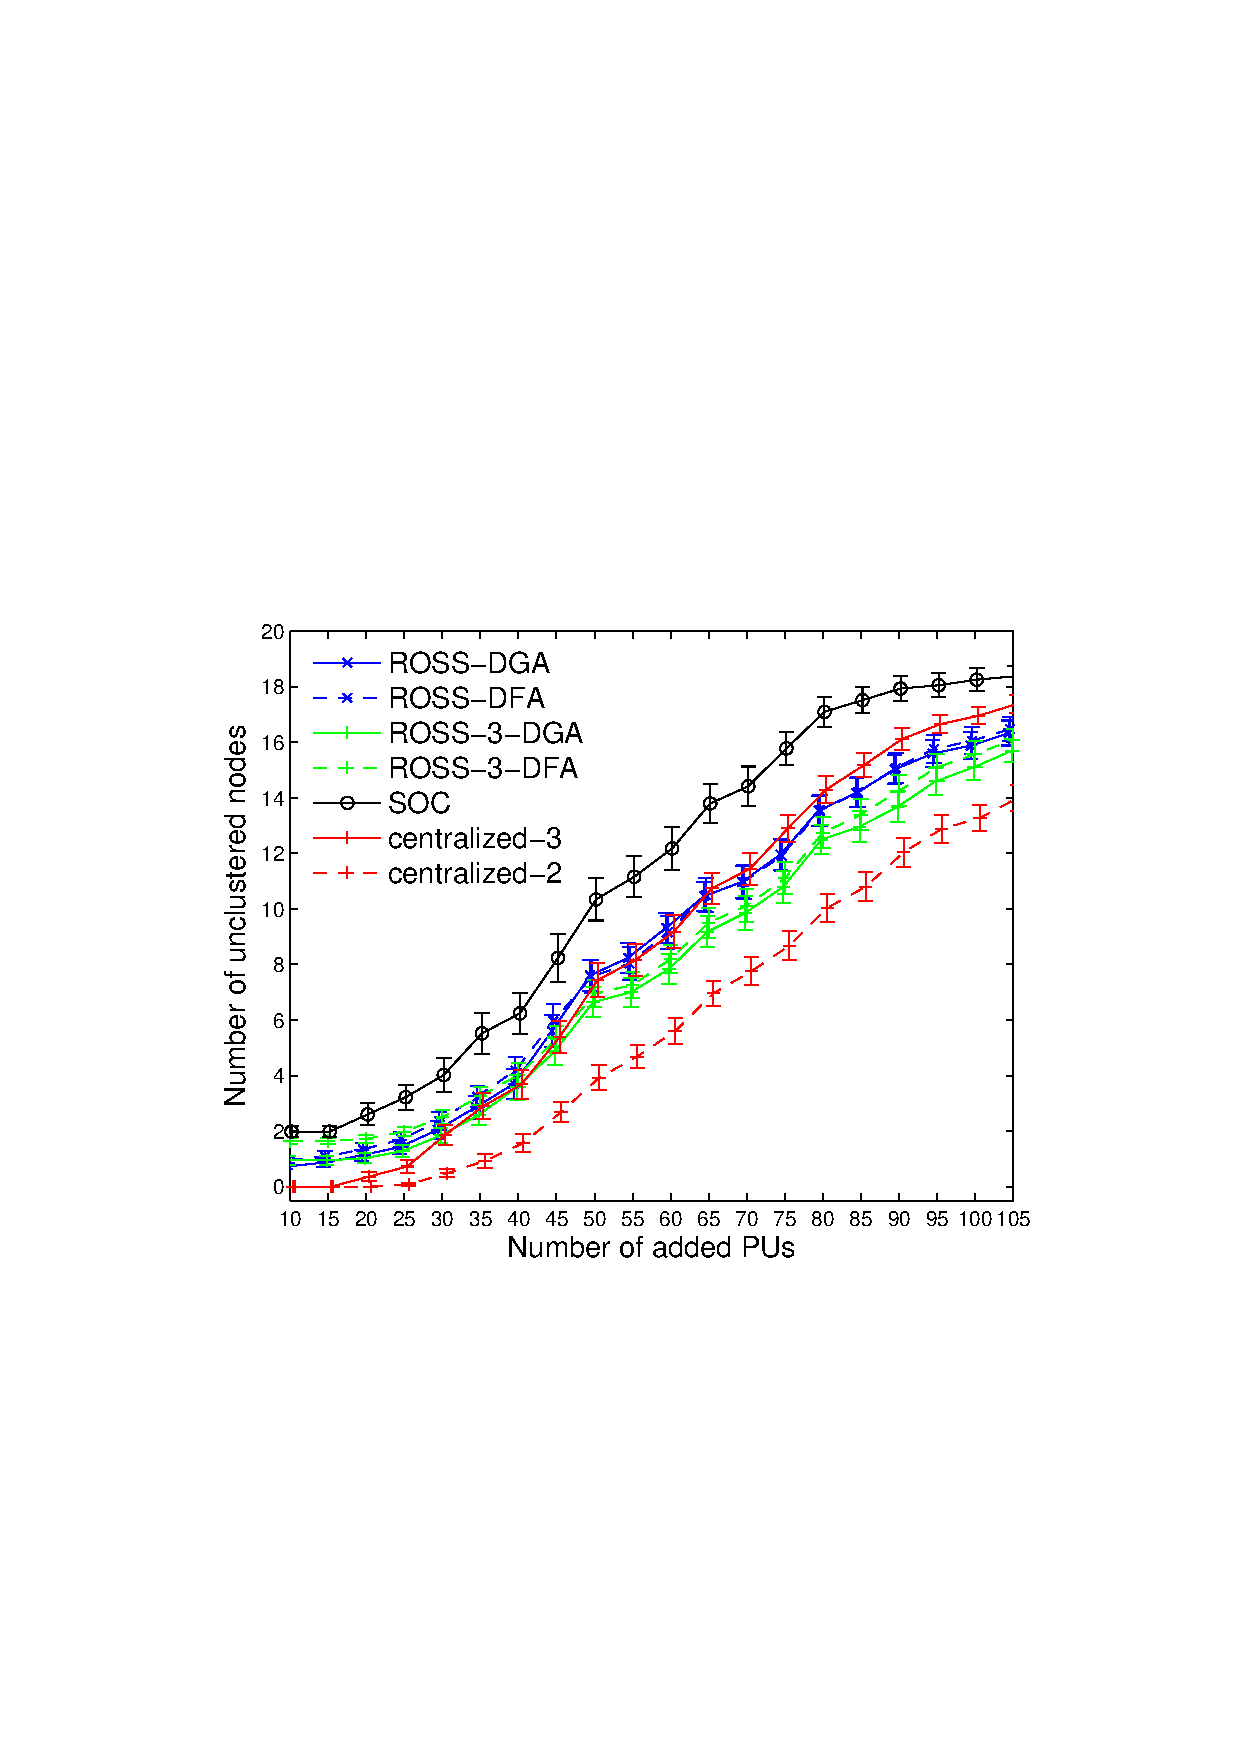
\includegraphics[width=0.7\linewidth]{survival_rate_20.pdf}
  \caption{Number of unclustered CRs with decreasing spectrum availability}\label{singleton_clusters}
\end{figure}


%\begin{figure*}[th]
%\begin{multicols}{3}
%    \includegraphics[width=\linewidth]{ccc_20.pdf}\par\caption{Number of common channels of non-singleton clusters}\label{ccc_per_nonsingleton}
%    \includegraphics[width=\linewidth]{cdf_clusterSize_20.pdf}\par\caption{Cumulative distribution of CRs residing in clusters with different sizes}\label{size_control}    
%    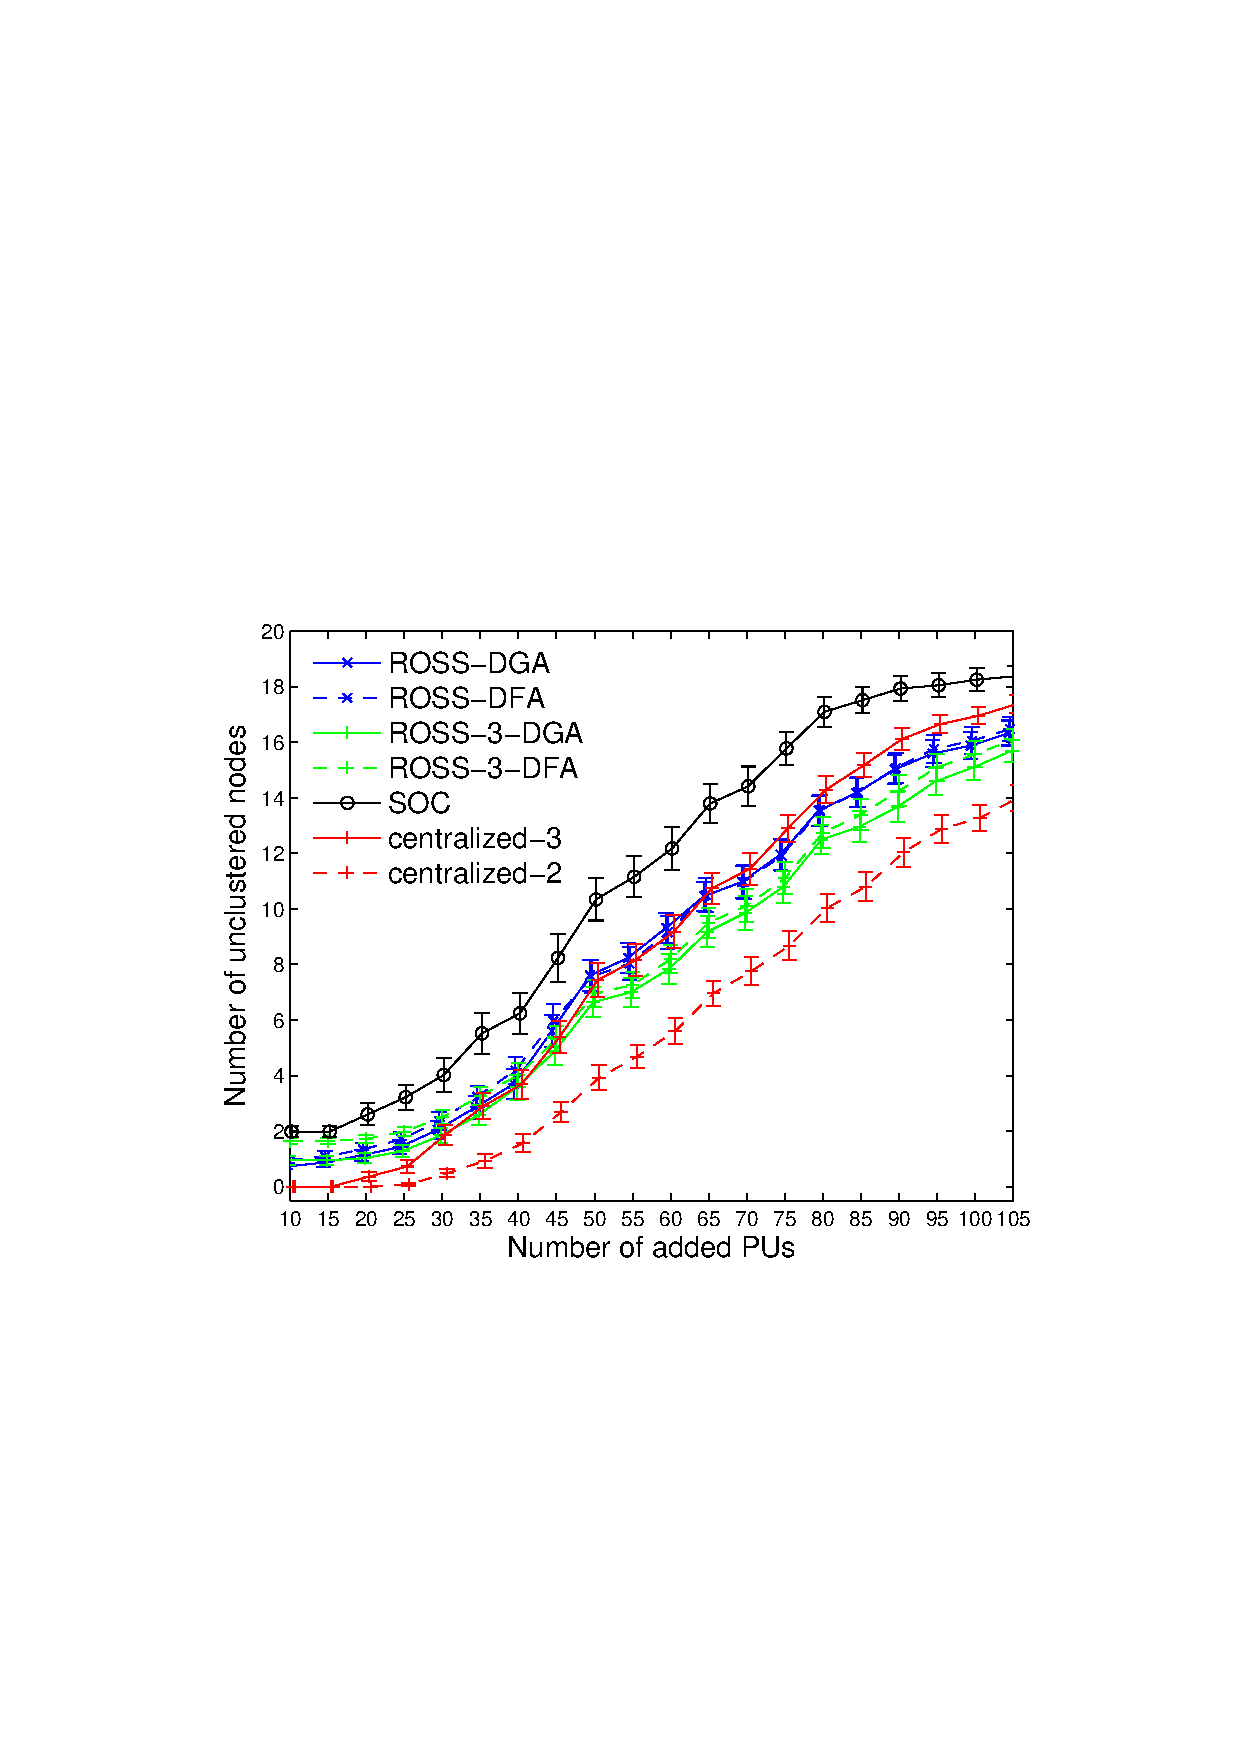
\includegraphics[width=\linewidth]{survival_rate_20.pdf}\par\caption{Number of unclustered CRs with decreasing spectrum availability}\label{singleton_clusters}
%\end{multicols}
%\caption{Comparison between the distributed and centralized clustering schemes ($N$ = 20)}
%\label{compare_dis_centralized}
%\end{figure*}



\subsubsection{Cluster Size Control}
\label{cluster_size}
%\begin{figure}[h]
%  \centering
%  \includegraphics[width=0.8\linewidth]{cdf_clusterSize_20.pdf}
%  \caption{Cumulative distribution of CRs residing in clusters with different sizes.}
%  \label{size_control}
%\end{figure}

Figure~\ref{size_control} depicts the empirical cumulative distribution of the CRs residing in certain sized clusters, from which we have two conclusions.
The first, SOC generates more unclustered CR nodes than other schemes.
The centralized schemes produce no unclustered CR nodes, ROSS-DGA/DFA generate 3\% unclustered nodes, as comparison, 10\% of nodes are unclustered when applying SOC.
ROSS-DGA and ROSS-DFA with size control feature generate 5\%-8\% unclustered CR nodes, which is due to the cluster pruning procedure (discussed in section~\ref{cluster_pruning}).
Second, the centralized schemes and cluster size control mechanism of RPSS generate clusters which satisfy the requirement on cluster size strictly.
%When the desired size is 2, each generated cluster has two members, whereas when the desired size is 3, about 15\% CRs are formed into 2 node clusters.
As to ROSS-DFG and ROSS-DFA with size control feature, CR nodes reside averagely in clusters whose sizes are 2, 3 and 4.
%When ROSS-3-DFA is applied, most number of CRs are in 3 node clusters, nevertheless, slightly less nodes are found in 2 node and 4 node clusters, there are also considerable number of singleton clusters.
%ROSS-3-DGA decreases the clusters sizes and results in more 2 node clusters, the second most CRs are found in 3 node clusters.
The sizes of clusters resulted from ROSS-DGA and ROSS-DFA are disperse, but appear to be better than SOC, i.e., the 50\% percentiles for ROSS-DGA, ROSS-DFA and SOC are 4.5, 5, and 5.5, and the 90\% percentiles for the three schemes are 8, 8, and 9.
%Figure~\ref{size_control} shows distributed clustering schemes are not able to control cluster sizes perfectly, but ROSS-DGA and ROSS-DFA eliminate the clusters whose size diverges largely with the desired one, \ie single node clusters and clusters with size of 13 and 14.



\subsubsection{Robustness of the clusters against newly added PUs}
%When the number of PUs in CRN increases, or their operation becomes more intensive, some clusters don't seize any CCCs any more, so that the cluster members and the cluster heads become unclustered, or singleton clusters.
%If there is no common control channels available any more because of the new added PRs, the cluster is regarded as destroyed and the former cluster member CRs become unclustered CRs or in other words singleton clusters.
%We investigate the number of singleton clusters with primary users whose intensity of activities are varying.
%We will obtain two observations by examining this metric.
%First, we will know how many CR nodes are unclusterred by applying the robust clustering schemes in a given CRN.
We add PUs in the CRN to decrease the available spectrum, and observe the number of unclustered CR nodes.
Clusters are formed with the presence of 10 PUs in the beginning, then extra 20 batches of PUs are added sequentially, where each batch includes 5 PUs. 
%The transmission range and channel occupancy of the new PU is the same with the previous ones, \ie transmission range is $A/3$, and one channel out of 10 is randomly chosen to operate.

Figure~\ref{singleton_clusters} shows with the increase of PUs, certain clusters disappear and the number of unclustered CR nodes increases.
Among the robust clustering schemes, the centralized scheme with desired size of two generates the most robust clusters, meanwhile, SOC results in the most vulnerable clusters.
The centralized scheme with desired size of three doesn't outperform the variants of ROSS, because the centralized scheme peruses clusters with size of 3 at the expenses of sanctifying CCCs.
In contrary, the variants of ROSS generate some smaller clusters which are more likely to survive when PUs' activities become intense.
%The comparison on cluster sizes will be given in Section~\ref{cluster_size}.
% when the number of PRs is 10$\sim$30, when number of PUs is 30$\sim$60, same amount of unclustered CRs are generated with variants of ROSS.
%When there are 75 and more new PRs, centralized scheme with cluster size of 3 results in more unclustered CR nodes than variants of ROSS.
%ROSS with size control distinguishes itself as the size control avoid the appearance of the clusters with large size.

%As to the variants of ROSS, the greedy process in ROSS improves the performance. 

%Greedy strategy adopted in the second phase of ROSS improves the robustness of clusters, i.e. ROSS-DGA exceeds ROSS-DFA, and ROSS-$\delta$-DGA surpasses ROSS-$\delta$-DFA.
%When the debatable CRs greedily update their affiliations, one of the metrics is the maximum increase of CCCs of the demanding clusters. 
%This observation complies with the result shown in Figure~\ref{ccc_per_nonsingleton}.
%Meanwhile, sizes of more clusters become smaller also contributes more robustness.


%\begin{figure}[h!]
%  \centering
%  \includegraphics[width=0.8\linewidth]{ccc_20.pdf}
%  \caption{Number of common channels for non-singleton clusters, the numbers in the names of schemes annotate the desired cluster size.}
%  \label{ccc_per_nonsingleton}
%\end{figure}
%
%
%\begin{figure}[h]
%  \centering
%  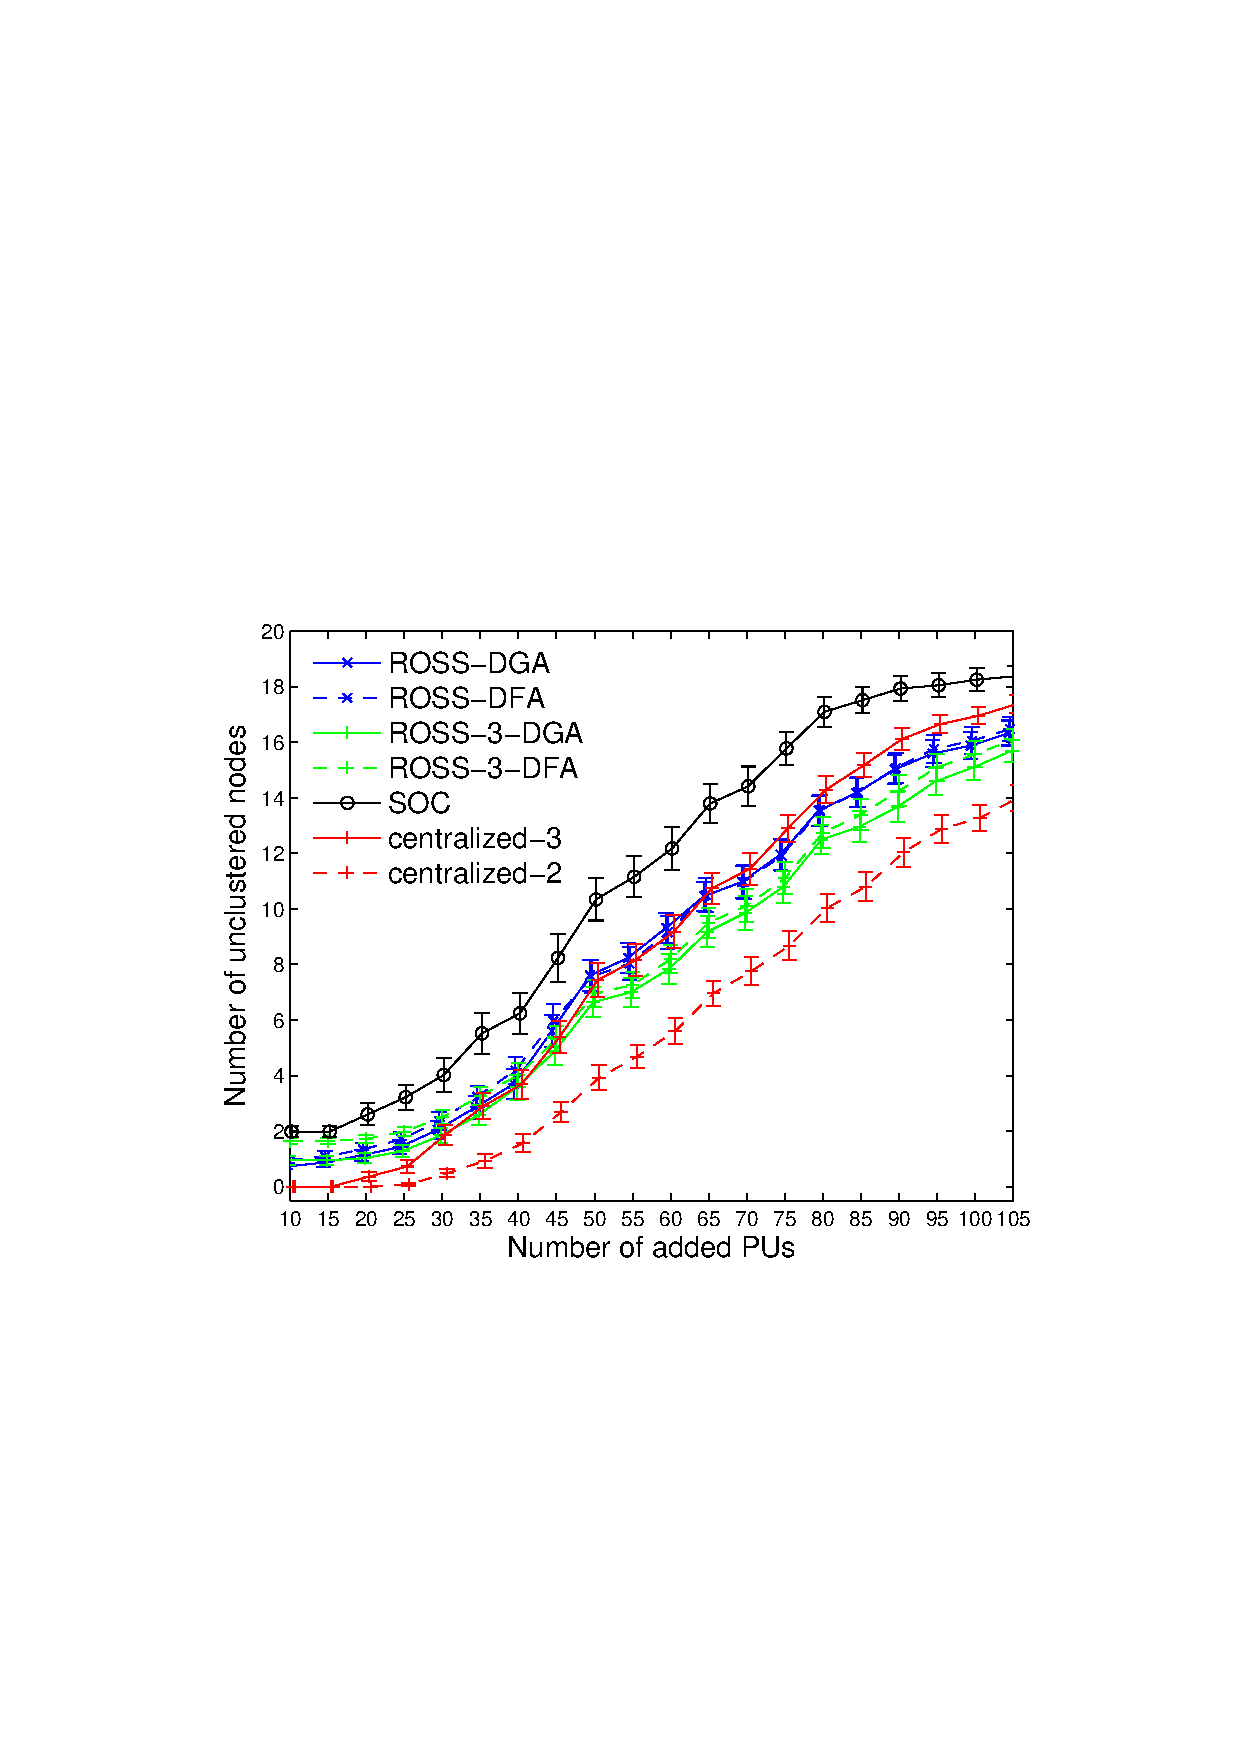
\includegraphics[width=0.8\linewidth]{survival_rate_20.pdf}
%  \caption{Number of CRs which are not included in any clusters}
%  \label{singleton_clusters}
%\end{figure}



\subsubsection{Control Signalling Overhead}
%Different from the clustering schemes proposed in ~\cite{LIU_TMC11_2, clustering_globecom11}, 
%There are two phases for any variants of ROSS.
%Clusters are formed in the first phase, in the second phase, cluster membership is decided so that each node only resides in one cluster.
%Control message exchanges between CR nodes are involved in both phases.

In this section we compare the overhead of signalling involved in different clustering schemes.
%In order to highlight the amount of control signalling only for clustering, 
We omit the control messaged involved in neighbourhood discovery, which is the premise for any clustering scheme.
According to~\cite{complexity_aggregation_2011}, the message complexity is defined as the number of messages used by all nodes.
To have the same criterion to compare, we count \textit{the number of transmissions of control messages}, without distinguishing they are sent with broadcast or unicast.
This metric is synonymous with \textit{the number of updates} discussed in Section~\ref{ross}.

As to ROSS, the control messages are generated in both phases.
In the first phase, when a CR node decides itself to be the cluster head, it broadcasts a message containing its ID, cluster members and the set of CCCs in its cluster.
%As to ROSS with size control feature, there are same amount of cluster heads with ROSS without enabling size control feature, and the cluster head broadcasts the available channels of the pruned cluster.
In the second phase, a debatable node broadcasts its affiliation to inform its claiming clusters, then the $\text{CH}$s of the claiming clusters  broadcast message about the new cluster members if they are changed due to the debatable node's decision.
The total number of the decisions involved in cluster formation has been analysed in Theorem~\ref{clustering:theorem} and Section~\ref{clustering:phaseII:game} respectively.

Comparison scheme SOC involves three rounds of execution. 
In the first two rounds, every CR node maintains its own cluster and seek to integrate neighbouring clusters, or joins one of them.
The final clusters are obtained in the third round. 
In each round, every CR node is involved in comparisons and cluster mergers.
%Comparing with the second phase of ROSS, only debatable nodes to communicate with cluster heads to clarify their membership.
%The signalling overhead for centralized scheme comes from two processes, the the process of collecting information to the centralized controller, and the process that the controller spreads the clustering result to all the CR nodes.

The centralized scheme is conducted at the centralized control device, but it involves two phases of control message transmission.
The first phase is information aggregation, in which every CR node's channel availability and neighborhood is transmitted to the centralized controller.
The second phase is broadcasting, where the clustering solution is disseminated to every CR node.
%
We adopt the algorithm proposed in~\cite{Efficient_broadcasting_gathering_adhoc} to broadcast and gather information as the algorithm is simple and self-stabilizing.
This scheme needs building a backbone structure to support the communication, and we apply ROSS to generate cluster heads which serve as the backbone, besides, the debatable nodes as used as the gateway nodes between the backbone nodes.
As the backbone is built once and support transmission for multiple times, the messages involved in the clustering process are not counted.
As to the process of information gathering, we assume that every cluster member sends the spectrum availability and its ID to its cluster head, which further forwards or the message to the controller, thus the number of transmission is $N$.
As to the process of dissemination, in an extreme situation where all the gateway and the backbone nodes broadcast, the number of transmission is $h + m$, where $h$ is the number of cluster heads and $m$ is number of debatable nodes.
%, $d$ is the average number of demanding clusters for each debatable node.

The number of control messages which are involved in both ROSS and the centralized scheme is related with the number of debatable nodes.
Figure~\ref{percentage_overlapping_node} shows the percentage of debatable nodes when the CRN network becomes denser, from which we can obtain the value of $m$.
\begin{figure}[ht!]
  \centering
  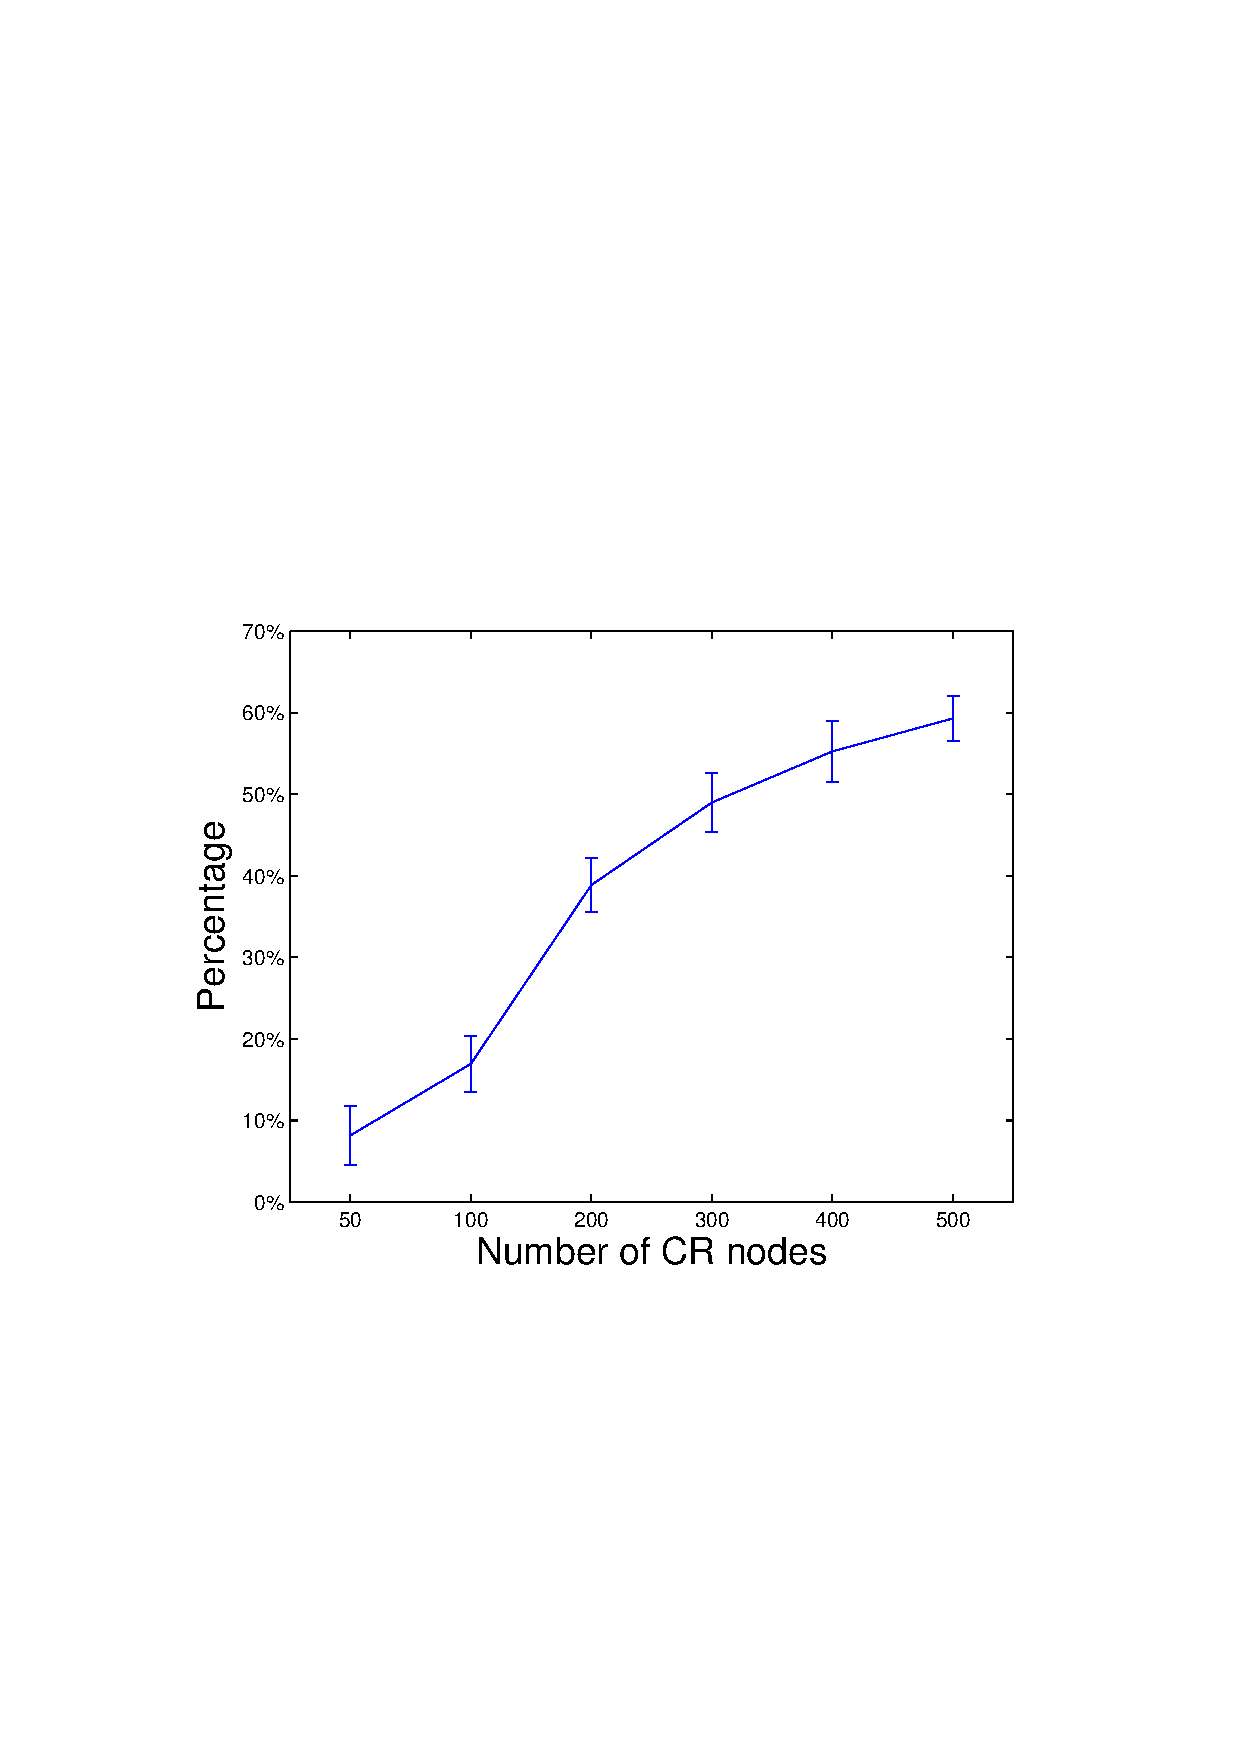
\includegraphics[width=0.6\linewidth]{percentage_overlapping_node.pdf}
  \caption{The percentage of debatable nodes after phase I of ROSS.}\label{percentage_overlapping_node}
\end{figure}
%
%As we adopt a simplified communication model, node's transmission is not influenced by collision or interference, 
%Our simulation doesn't consider the behaviour in the physical layer, 
%
%
%Assume we use OSPF~\cite{BCJ10} to aggregate and disseminate information, then the best and worst complexity for is $\mathcal{O}(E)$, where $E$ is the number of edges in the graph which corresponds to the network.
%The minimum number of edges is $n-1$ when the nodes form a line and each node has at more two neighbours, and the maximum number is $N*(N-1)/2$ when the nodes form a complete graph.
%Thus the best message complexity of the centralized scheme is $\mathcal{O}{(N)}$ and the worst is $\mathcal{O}{(N^2)}$.
%
%1. update membership to form X1, 
%2. broadcast new X1, form new X2
%3. broadcast X3
%The complexity parameters are the number of nodes $n$ in network, number of clusters $h$.
The message complexity, quantitative analysis of the number of control messages involved in clustering, and the size of control messages are shown in Table \ref{tab_overhead}.
%$D(s)$: the maximum distance between centralized controller and CR users.
%
Figure~\ref{control_msg} shows the number of transmissions of SOC, the upper bound of the number of transmissions for ROSS, and the analytical number of transmissions of the centralised scheme. 
%Note that the curve for the centralized scheme is from theoretical analysis, which is $h+m+N$ as discussed beforehand.
%Note the overhead involved to construct the backbone (clusters) is not included.




%\begin{table}[hc]
%\centering
%\caption{Singalling overhead. Notations: $n$-number of CR nodes in CRN, $h$-number of cluster heads, $m$-number of debatable nodes, $c$-number of demanding clusters.}\label{tab_overhead}
%\begin{tabular}{|p{2.2 cm}|p{1.5 cm}|p{3.7 cm}|}
%\hline
% Scheme 					&   Number of transmissions 					& Content of message \\ \hline
% ROSS-DGA, ROSS-$\delta$-DGA 		&   $h+2*m^2c$ (upper bound)
%				& $ID_{H_C}$ and $K_C$ for $h+m^2c$ times, notification to join one cluster for $m^2c$ times					\\ \hline
% ROSS-DFA, ROSS-$\delta$-DFA 		&   $h+ 2m$	 (upper bound) 						& $ID_{H_C}$ and $K_C$ for $h+m$ times, notification to join one cluster for $m$ times	 					\\ \hline
% SOC 						&   $3*n$					& $\{K_i\}, i\in M\subseteq \texttt{Nb}_i$						\\ \hline
% Centralized				&	$n$						& $\{C\}$         	\\ 
% \hline
%\end{tabular}
%\end{table}

\begin{center}
\begin{table*}[!htb]
\caption{Signalling overhead}\label{tab_overhead}
{\small
\hfill{}
\begin{tabular}{|L{2.2 cm}|C{2.8 cm}|C{3.15 cm}|C{6.6 cm}|}
\hline
 Scheme 				&Message Complexity 	&   Quantitative number of messages 		& Content of message (size of message) 									\\ \hline
 ROSS-DGA, ROSS-$\delta$-DGA 	&$\mathcal{O}(N^3)$ (worst case)		&   $h+2*m^2d$ (upper bound)  				&   \multirow{2}{*}{\parbox{6.4cm}{Phase I: notification from cluster head (1 byte), new individual connectivity degree (1 byte);  Phase II: update of debatable nodes' affiliation (1 byte), claiming cluster $i$' new membership ($|C(i)|$ bytes)}}								\\ \cline{1-3}
 ROSS-DFA, ROSS-$\delta$-DFA 	&$\mathcal{O}(N)$ (worst case)		&   $h + 2m$	 (upper bound) 					& 	      												\\ \hline
 SOC 					&$\mathcal{O}(N)$		&   $3*N$									& $C(i)$ ($|C(i)|$ bytes), $K(C(i))$ ($|\mathcal{P}|$ bytes), $i\in \mathcal{N}$						\\ \hline
 Centralized			&$\mathcal{O}(N)$			&	$h + m + N$ (upper bound)~\cite{Efficient_broadcasting_gathering_adhoc}		& $\{C\}$ ($|C_i|*N$ bytes)        					\\ \hline
\end{tabular}
}
\hfill{}
\end{table*}
\end{center}
% centralized: $\mathcal{O}(D(s)+log N)$ + $\mathcal{O}(1+D(s)+log N)$



\begin{figure}[ht!]
  \centering
  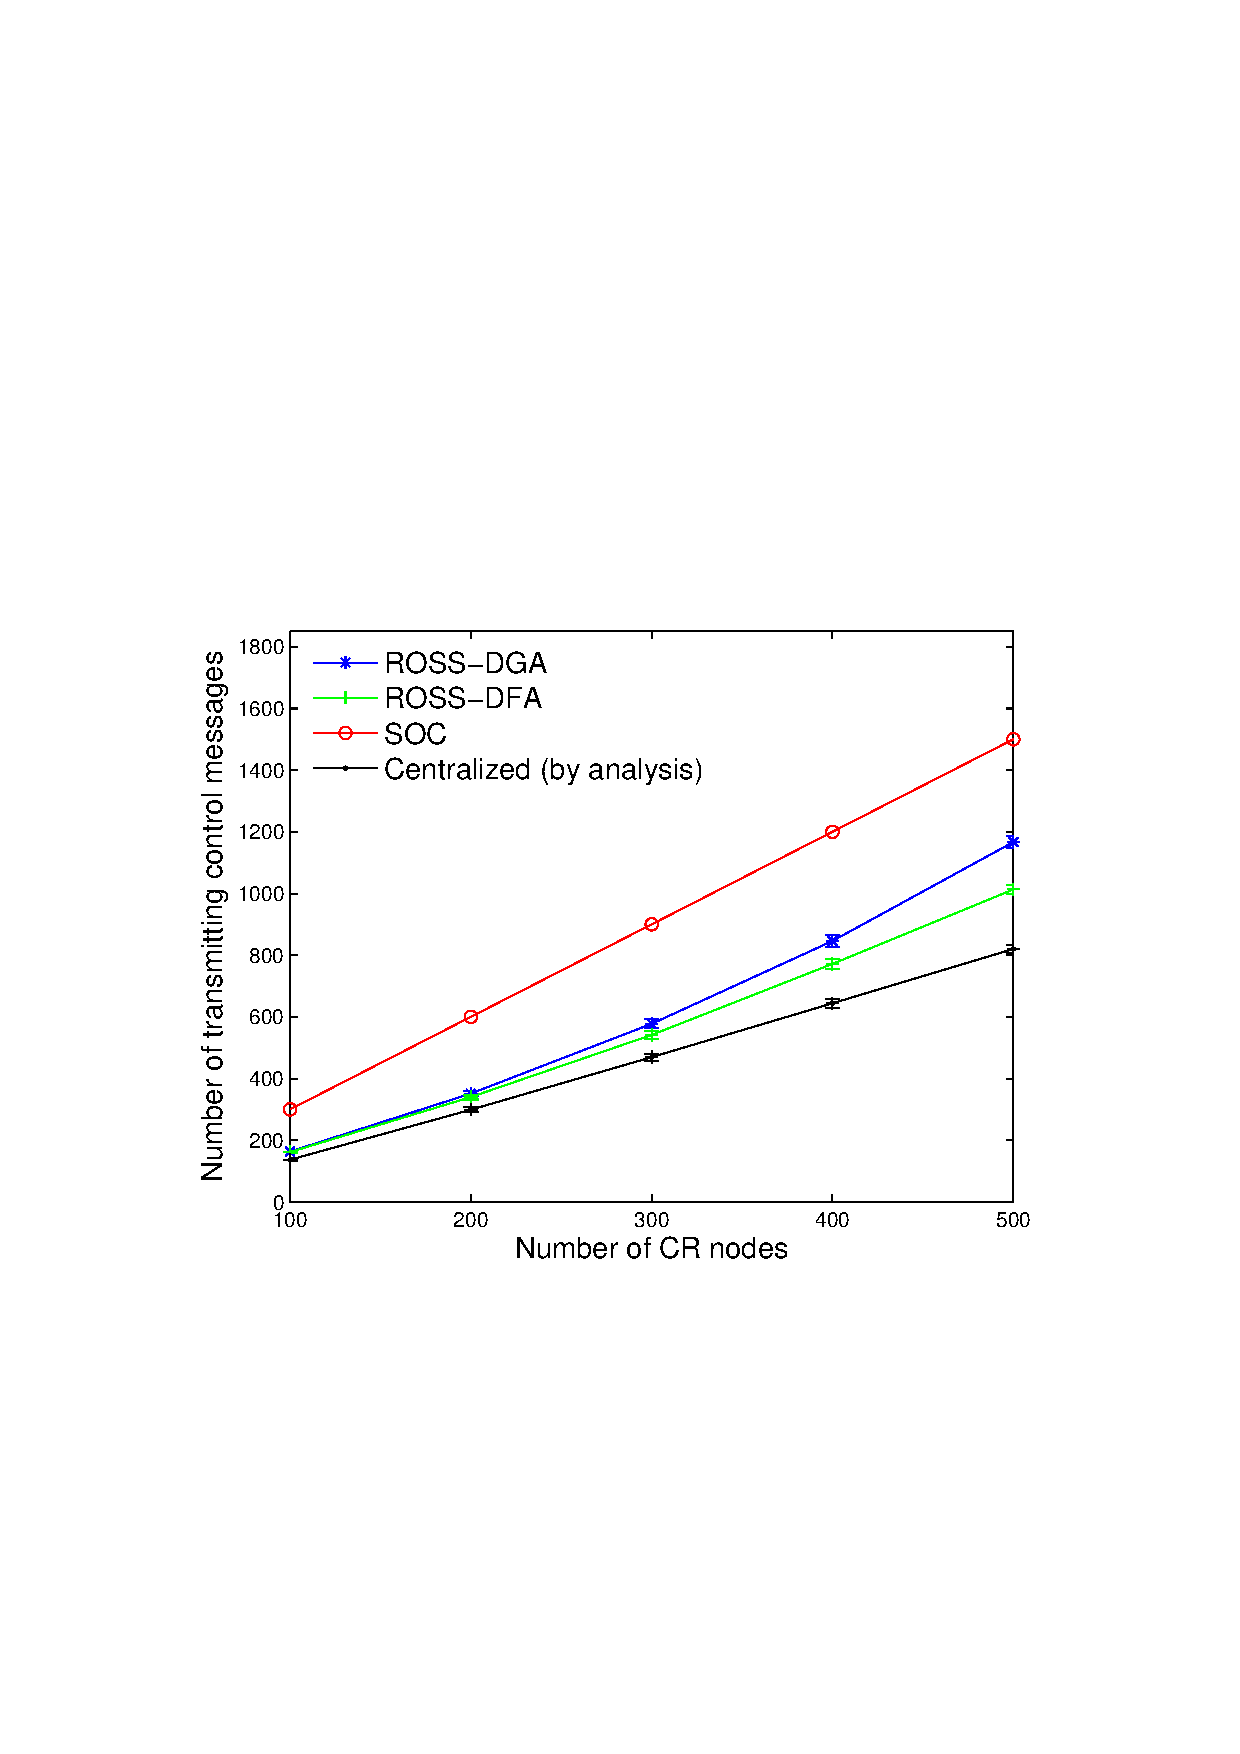
\includegraphics[width=0.7\linewidth]{number_controlMsg.pdf}
  \caption{Number of control messages. Note the curves of ROSS-DGA and ROSS-DFA are the upper bounds}
  \label{control_msg}
\end{figure}





\subsection{Comparison Between Distributed Schemes}
\label{largeScaleCRN}
In this section we investigate the performances of distributed clustering schemes in CRN with different network scales and densities.
The transmission range of CR is $A/5$, PR's transmission range is $2A/5$.
The initial number of PU is 30.
%The number of CR is 100, 200 and 300, and the average number of neighbours of each CR is 9.5, 20, and 31.
The desired sizes adopted are listed in the Table~\ref{Simulation_para}, which is about 60\% of the average number of neighbours.


\begin{table}[ht]
\caption{}
\label{Simulation_para}
{\small
\hfill{}
\begin{tabular}{|L{3.7 cm}|C{1 cm}|C{1 cm}|C{1 cm}|}
\hline
Number of CRs			& 100 	&  200 					& 300 \\ \hline
Average num. of neighbours 	&9.5	&   20		& 31  \\ \hline
Desired size $\delta$ 	& 6	&   12 						& 20      \\ \hline
\end{tabular}
}
\hfill{}
\end{table}



\subsubsection{Number of CCCs per Non-singleton Clusters}

\begin{figure}[ht!]
  \centering
  \includegraphics[width=.7\linewidth]{ccc_large_scale_color.pdf}
  \caption{Number of common channels of non-singleton clusters.}
  \label{ccc_large_scale}
\end{figure}

Figure~\ref{ccc_large_scale} shows the average number of CCCs of the non-singleton clusters.
We notice that SOC achieves the most CCCs per non-singleton cluster, although the lead over the variants of ROSS shrinks significantly when $N$ increases.
%\ie when $N=300$, the number of CCCs achieved by ROSS variants (except for ROSS-$\delta$-DFA) is almost the same as that resulted from SOC.
%This means SOC out performs in terms of the average number of CCCs per non-singleton cluster when network is sparse.
%This is also observed in the evaluation in Section \ref{ccc_20} where $N=20$.
%When the network becomes denser, even this metric favours SOC as discussed in the beginning of Section~\ref{performance}, ROSS-DGA achieves even more CCCs than SOC, and ROSS-DFA and ROSS-$\delta$-DGA increase the number of CCCs visibly.




\subsubsection{Robustness of the clusters against newly added PUs}
We add extra 20 batches of PUs sequentially in the CRN, where each batch includes 10 PUs. 
%In this part of simulation, we investigate the robustness of clusters by increasing the PUs working on certain channels.
Figure~\ref{singleton_clusters_100} and \ref{singleton_clusters_200} show that when $N=100$ and 200, more unclustered CR nodes appear in the CRN where SOC is applied.
When the network becomes denser, ROSS-DGA/DFA generate slightly more unclustered CR nodes than SOC when new PUs are not many, but SOC's performance deteriorates quickly when the number of PUs becomes larger.
We only show the average values of the variants of ROSS as their confidence intervals overlap.
%
When applying ROSS with size control mechanism, significantly less unclustered CR nodes are generated.
Besides, the greedy mechanism moderately strengthens the robustness of the clusters.
%It can be seen that greedy algorithms result in slightly less singleton clusters than their counterparts.
%
%Figure ~\ref{singleton_clusters_300} depicts a denser CRN where $N=300$.
%SOC noticeably causes more singleton clusters than ROSS variants, except that ROSS-20-DFA results in more singleton clusters when PUs are few.
%The reason is ROSS-20-DFA conducts cluster membership clarification for only once, which causes large number of singleton clusters.
%ROSS-20-DGA increases the size of smaller clusters through debatable nodes' repeated updates thus drastically decreases the number of singleton clusters.
%\begin{figure}[!h]
%  \centering
%  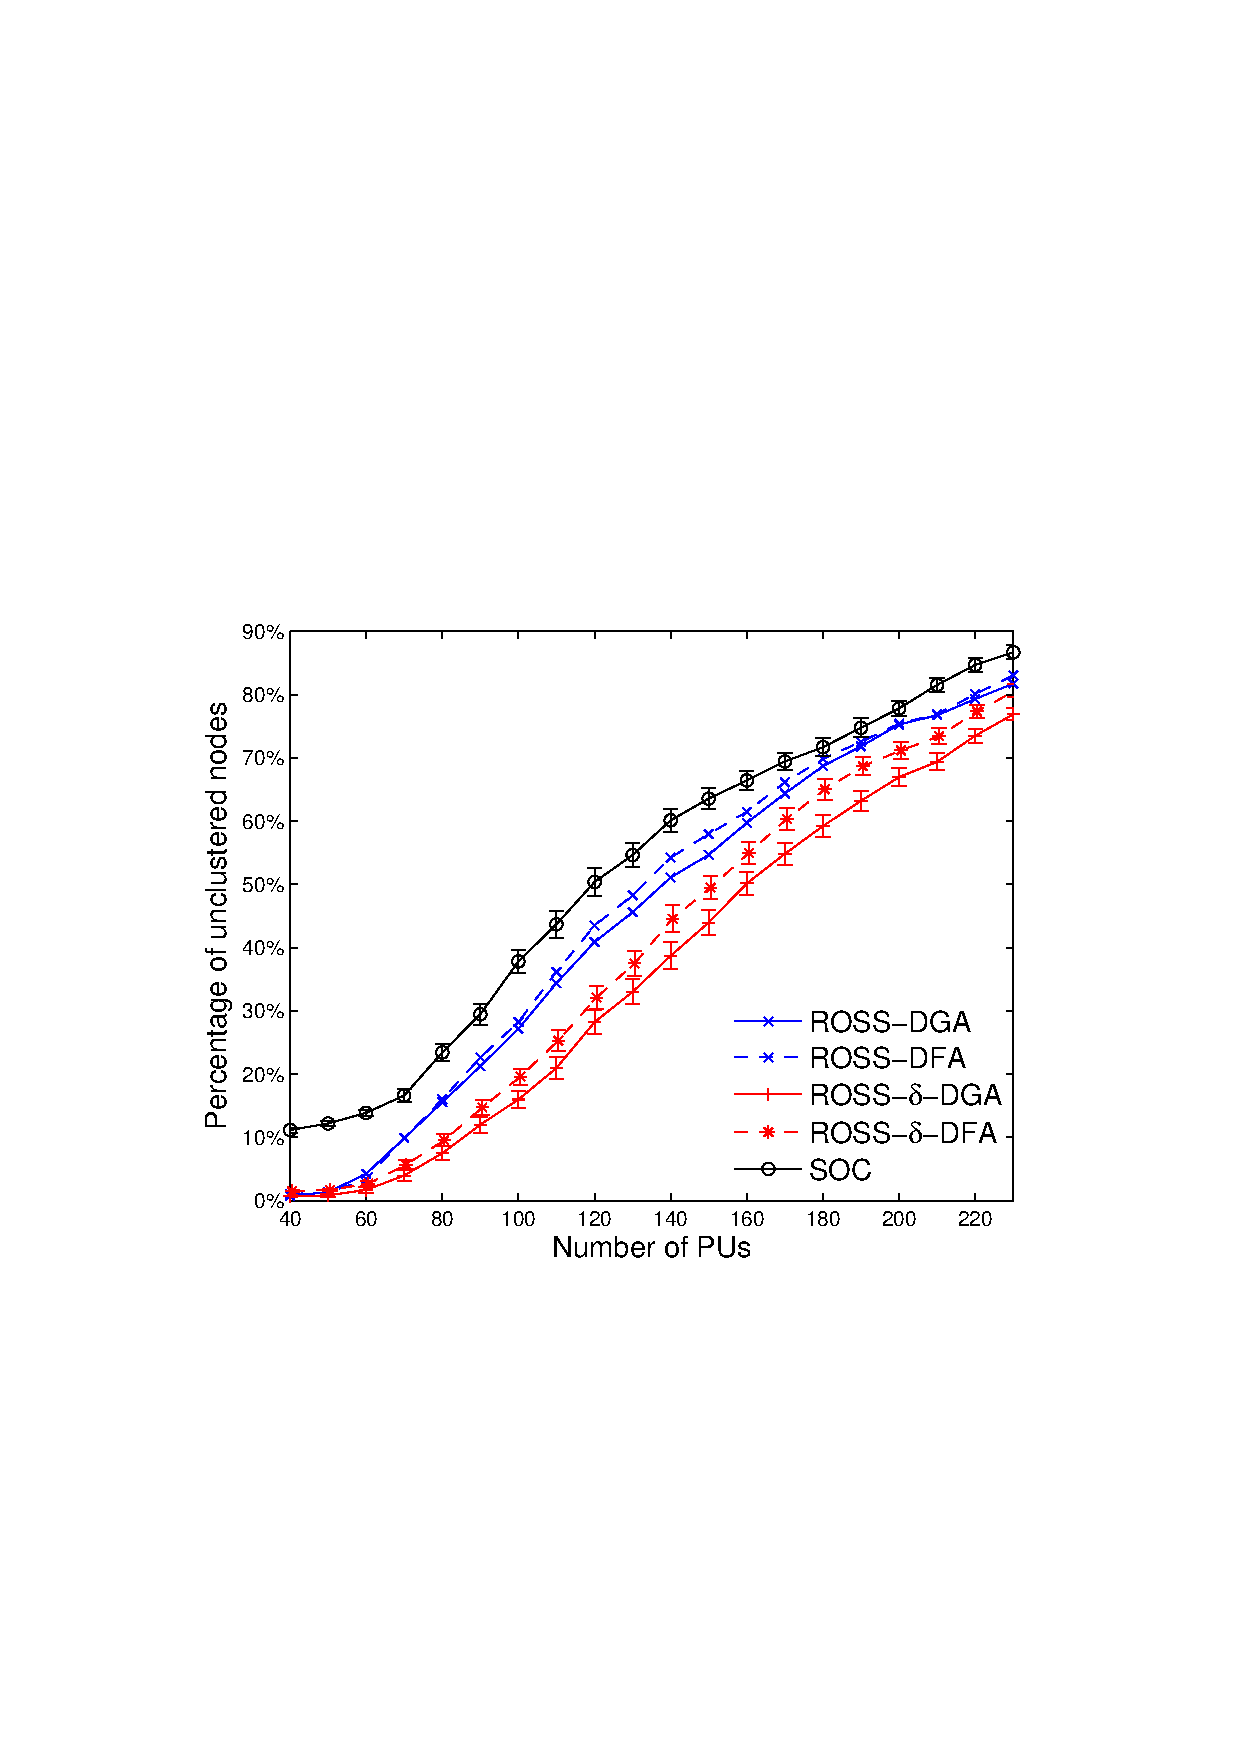
\includegraphics[width=0.7\linewidth]{survival_rate_100_edge50.pdf}
%  \caption{Percentage of CRs which are not included in any clusters with the increasing number of primary users, $N=100$}
%  \label{singleton_clusters_100}
%\end{figure}
%  
%  \begin{figure}[!h]
%    \centering
%   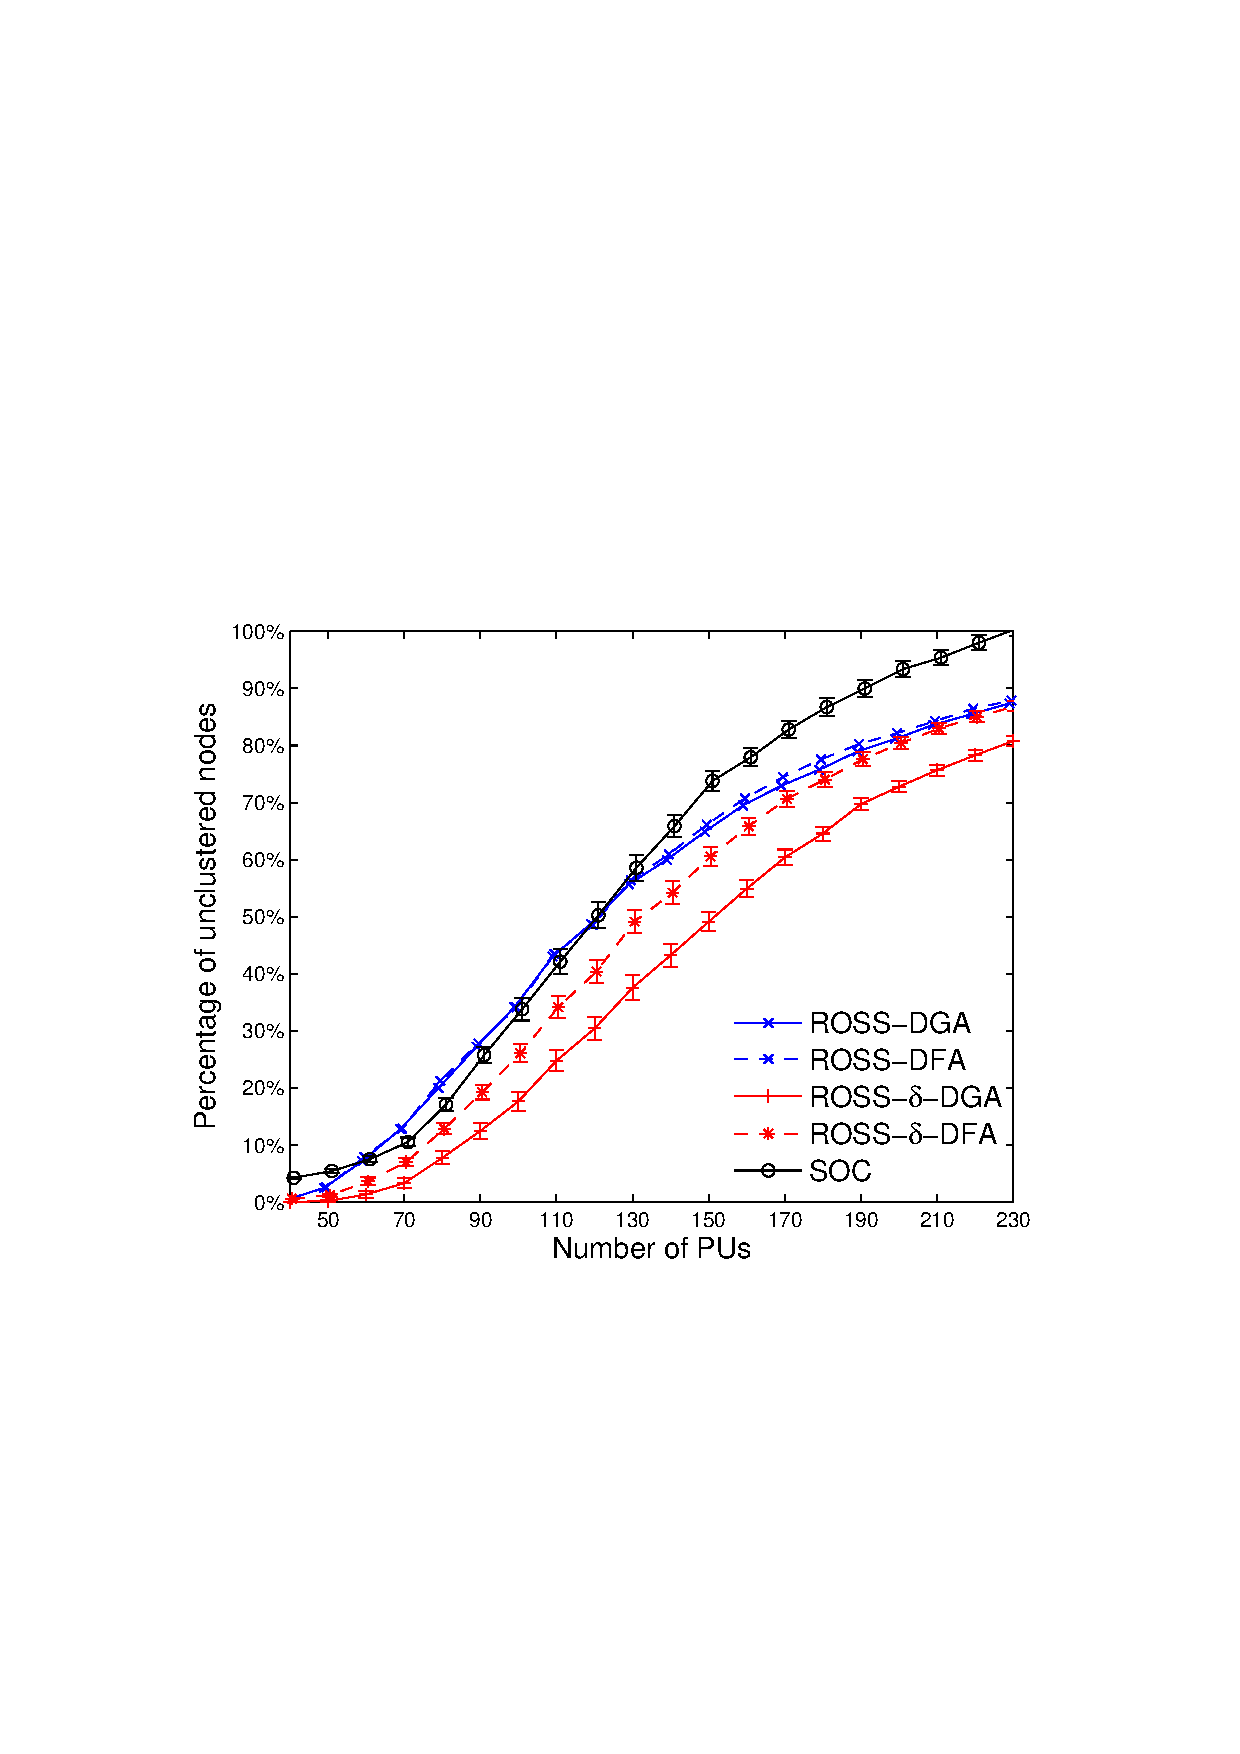
\includegraphics[width=0.7\linewidth]{survival_rate_300_edge50.pdf}
%  \caption{Percentage of CRs which are not included in any clusters with the increasing number of primary users, $N=300$}
%  \label{singleton_clusters_300}
%\end{figure}

\begin{figure}[ht!]
  \centering
  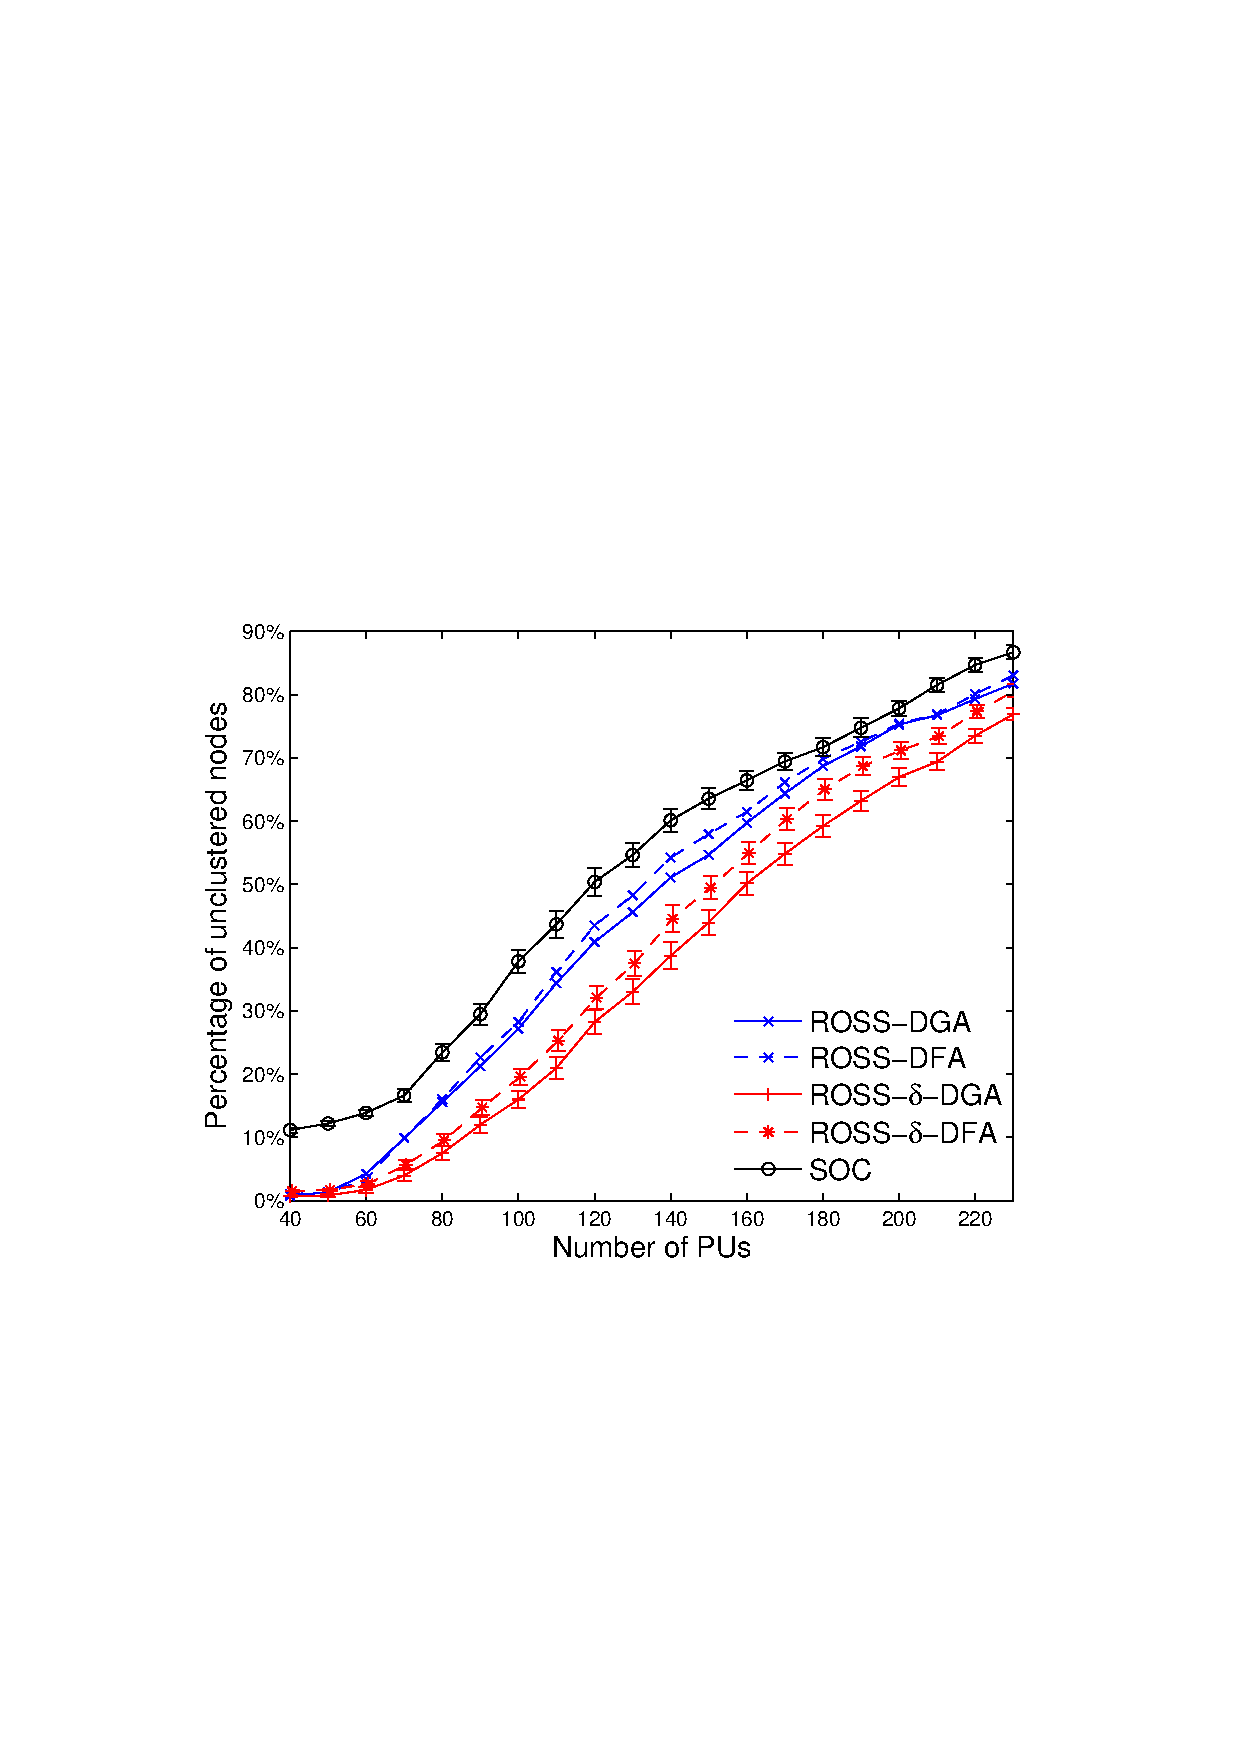
\includegraphics[width=.7\linewidth]{survival_rate_100_edge50.pdf}
  \caption{Percentage of CR nodes which are not included in any non-singleton clusters, 100 CRs}
  \label{singleton_clusters_100}
\end{figure}

\begin{figure}[ht!]
  \centering
  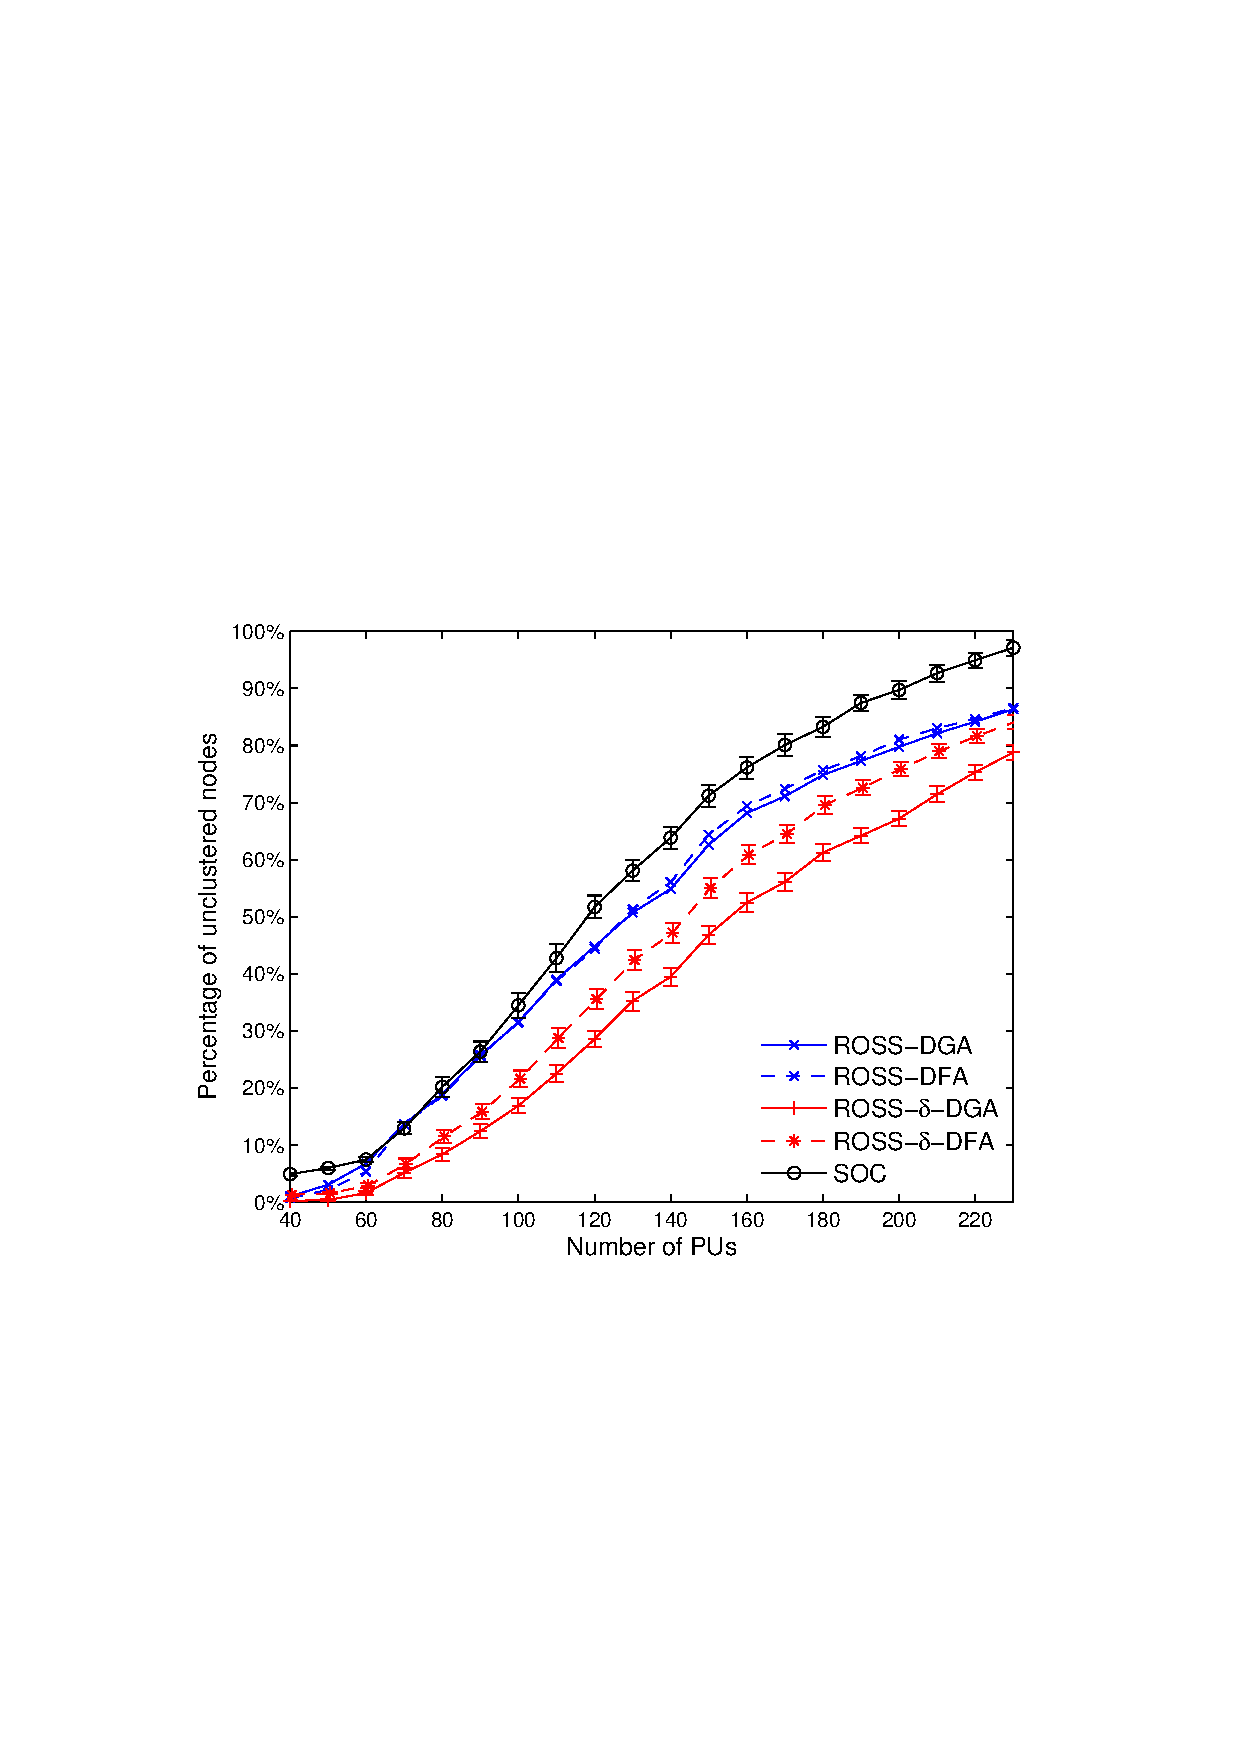
\includegraphics[width=.7\linewidth]{survival_rate_200_edge50.pdf}
  \caption{Percentage of CR nodes which are not included in any non-singleton clusters, 200 CRs}
  \label{singleton_clusters_200}
\end{figure}

\begin{figure}[ht!]
  \centering
  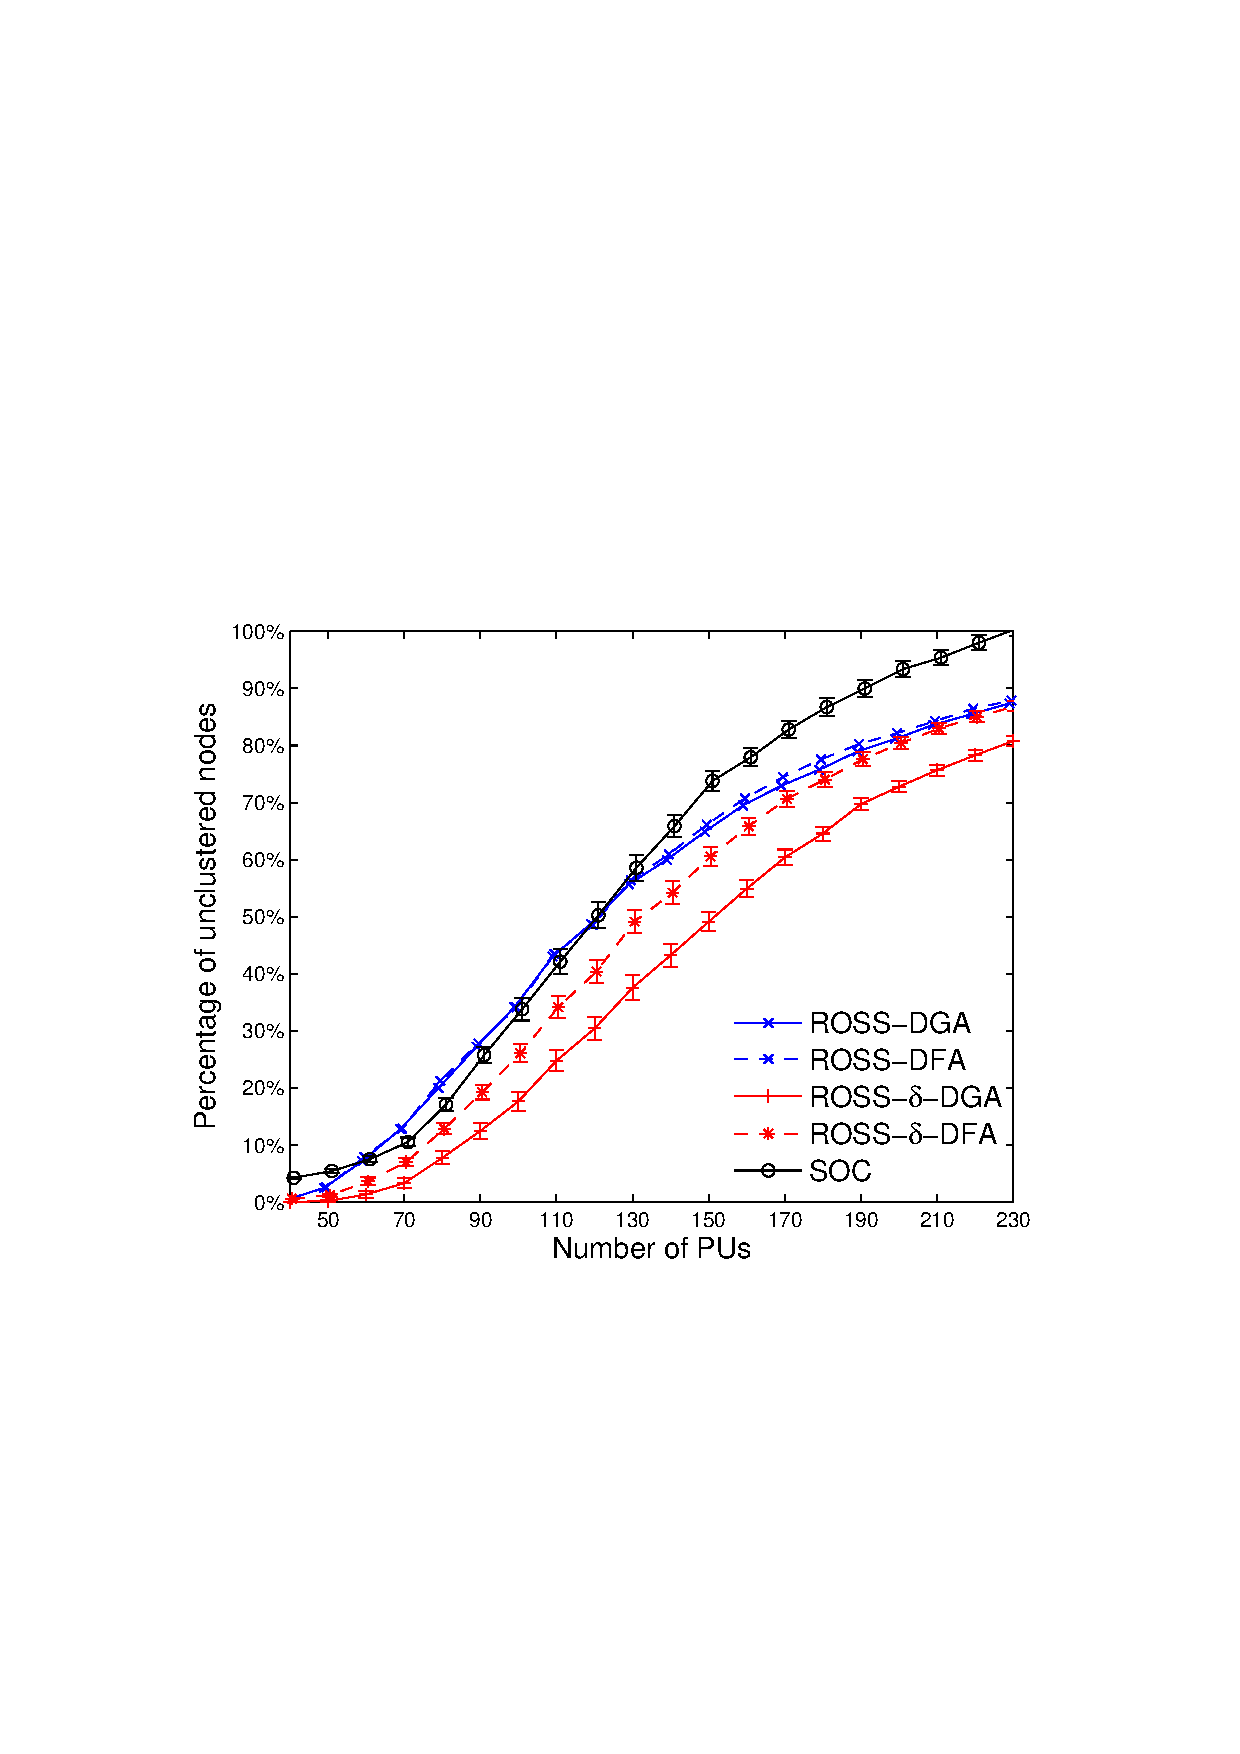
\includegraphics[width=.7\linewidth]{survival_rate_300_edge50.pdf}
  \caption{Percentage of CR nodes which are not included in any non-singleton clusters, 300 CRs}
  \label{singleton_clusters_300}
\end{figure}
%\begin{figure*}[t]
%\begin{multicols}{3}
%    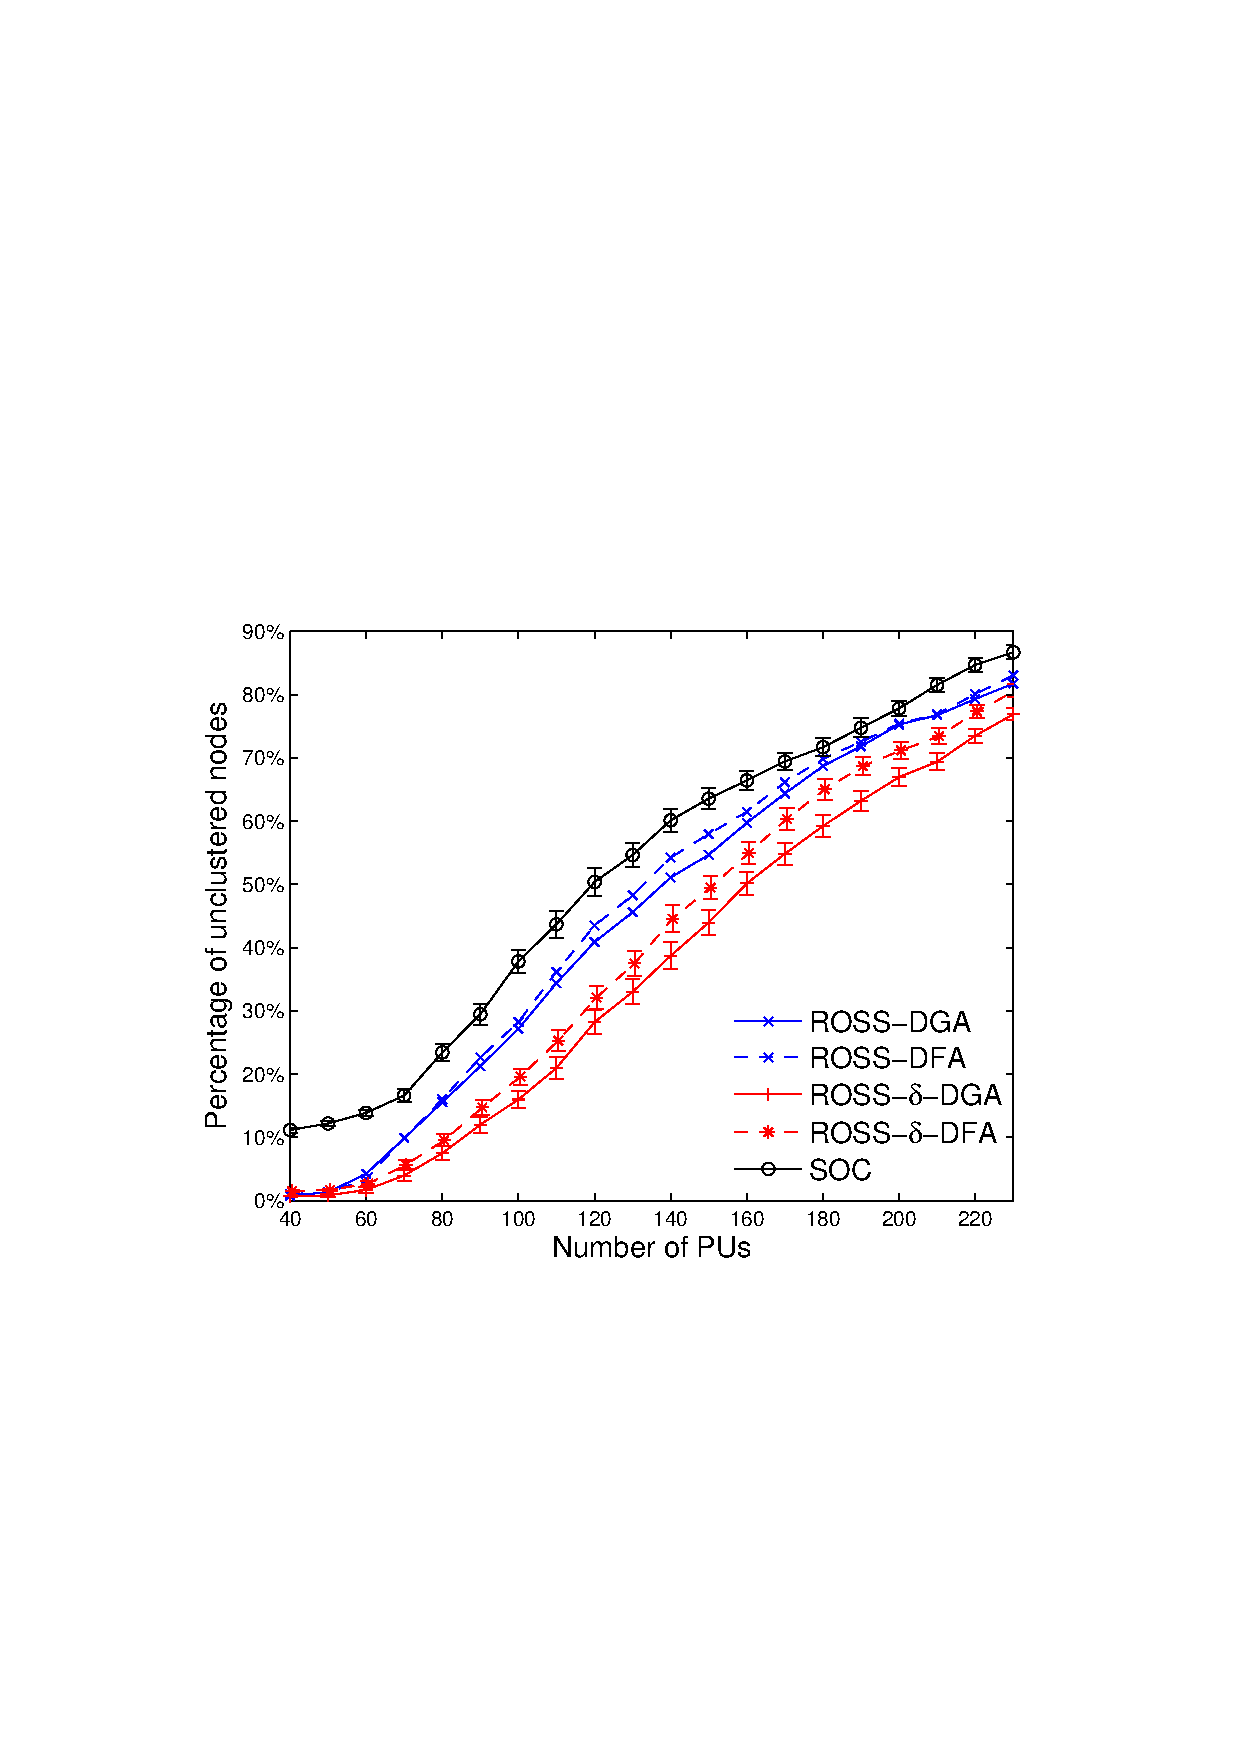
\includegraphics[width=\linewidth]{survival_rate_100_edge50.pdf}\par\caption{100 CRs}\label{singleton_clusters_100}
%    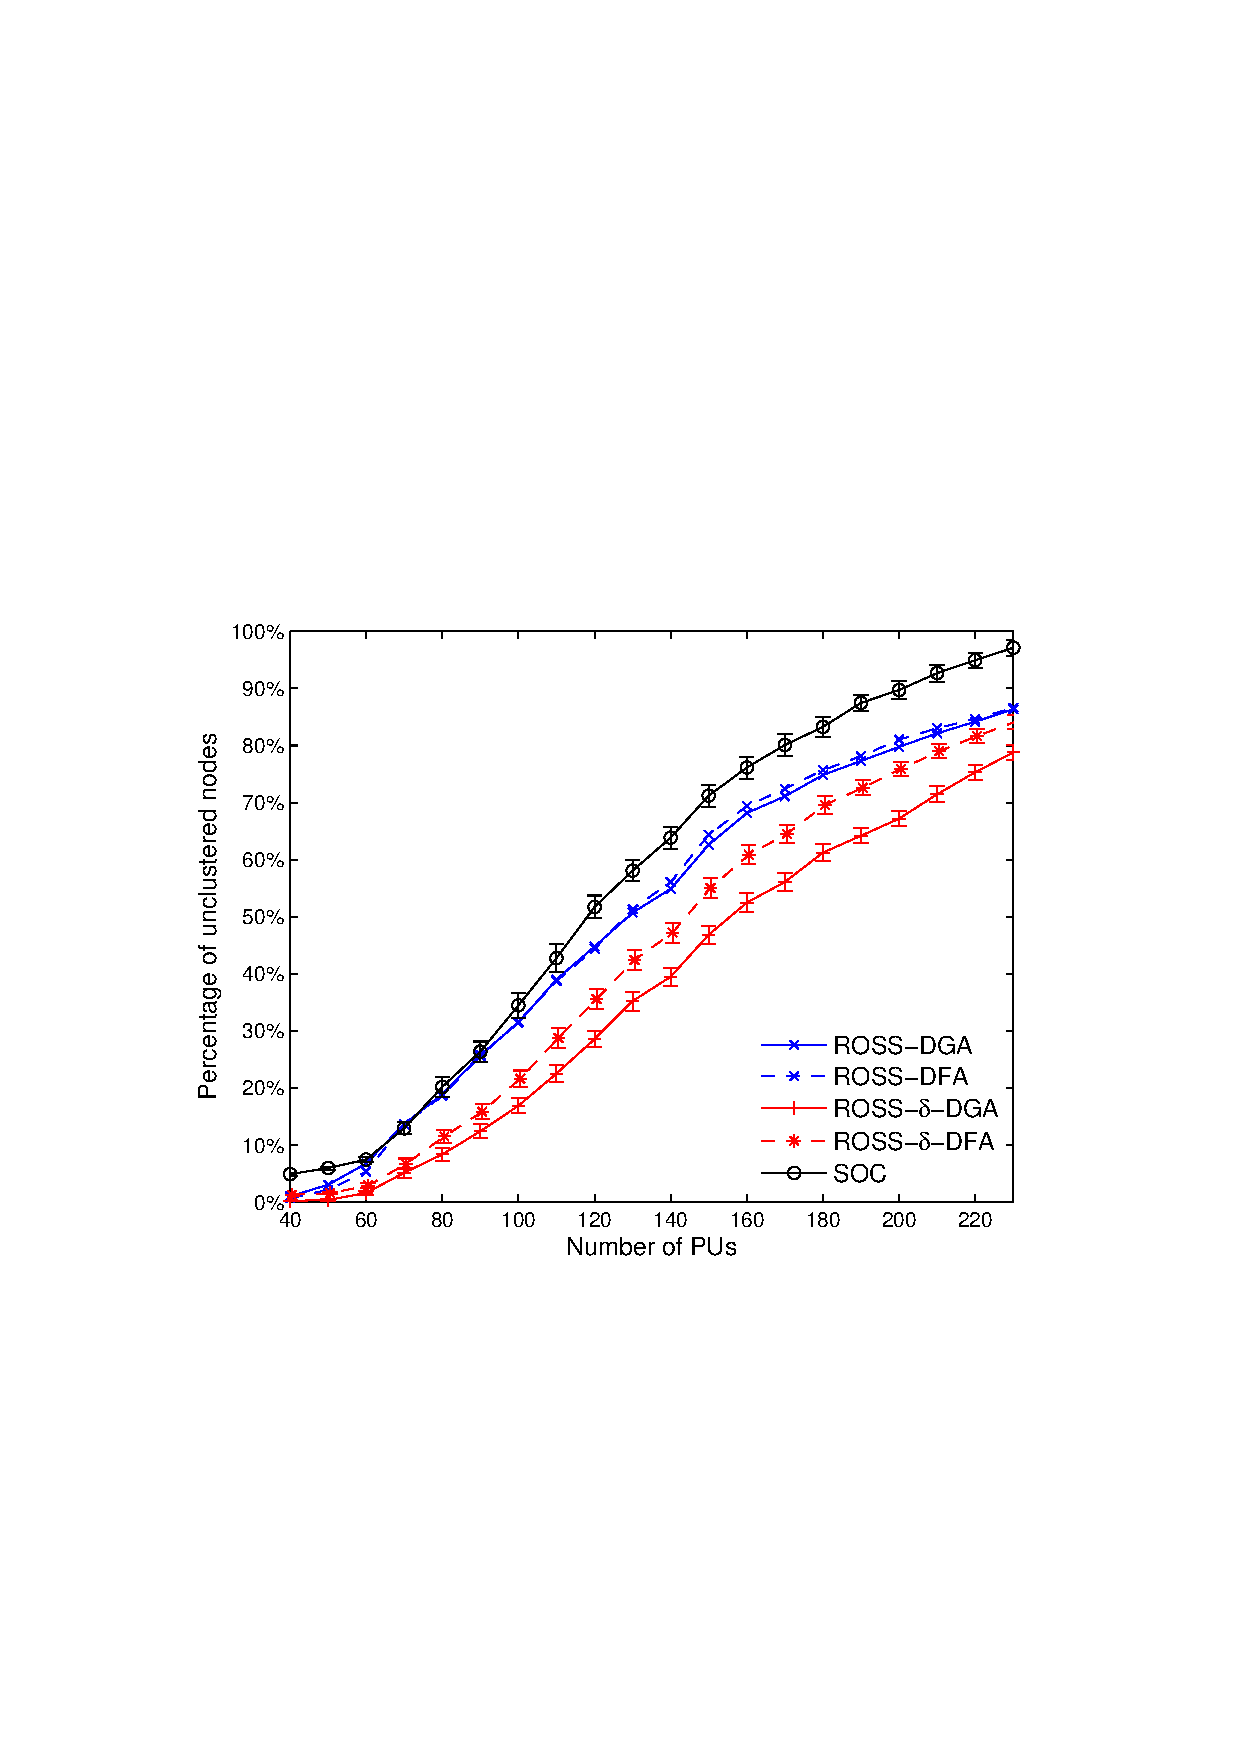
\includegraphics[width=\linewidth]{survival_rate_200_edge50.pdf}\par\caption{200 CRs}\label{singleton_clusters_200}
%    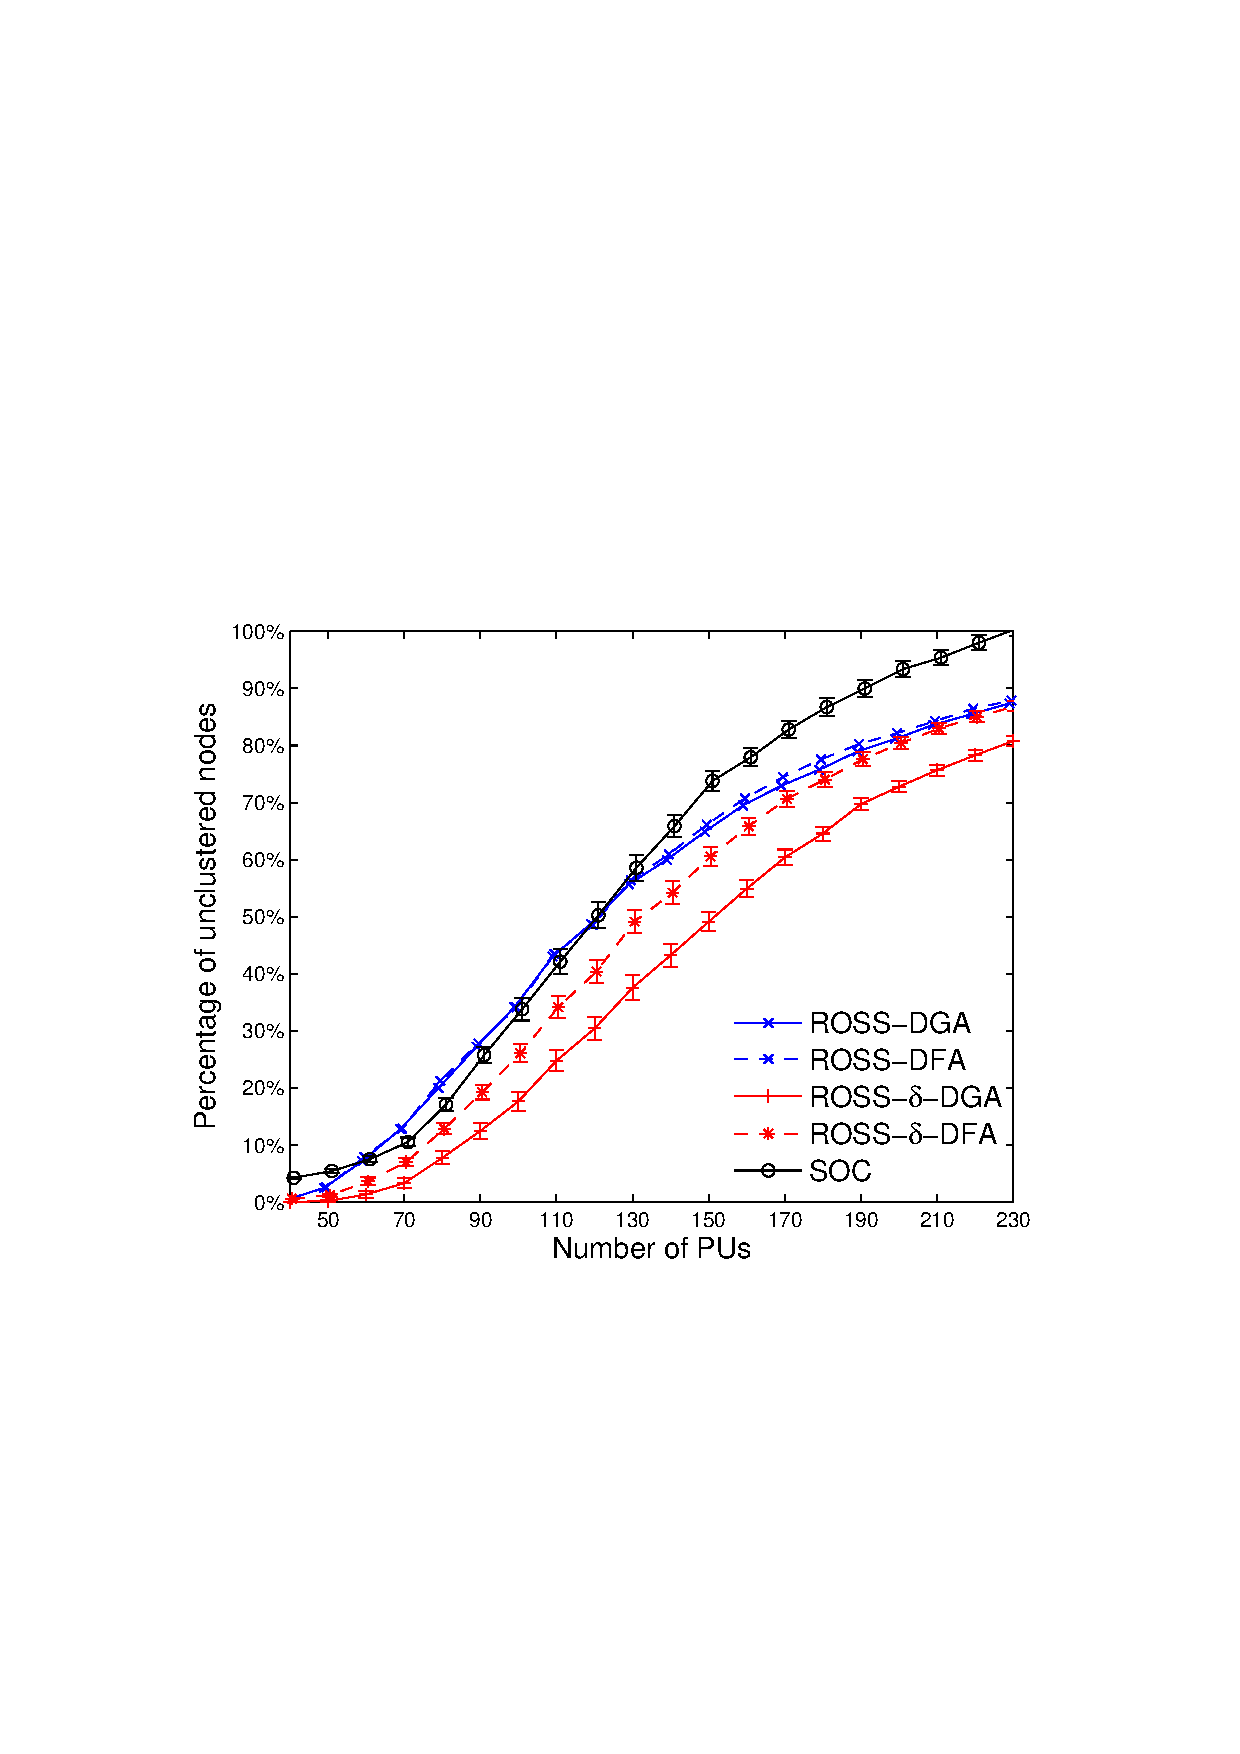
\includegraphics[width=\linewidth]{survival_rate_300_edge50.pdf}\par\caption{300 CRs}\label{singleton_clusters_300}
%\end{multicols}\caption{Percentage of CR nodes which are not included in any non-singleton clusters}
%\label{unclustered_100_200_300}
%\end{figure*}

%When the network is denser, the improvement on cluster sizes and robustness by the greedy search in the membership clarification phase is more obvious.


\begin{figure}[ht!]
  \centering
  \includegraphics[width=.7\linewidth]{cdf_clusterSize_100.pdf}
  \caption{Cumulative distribution of CRs residing in clusters with different sizes, 100 CRs, 30 PUs in network}
  \label{cdf_clusterSize_100}
\end{figure}

\begin{figure}[ht!]
  \centering
  \includegraphics[width=.7\linewidth]{cdf_clusterSize_200.pdf}
  \caption{Cumulative distribution of CRs residing in clusters with different sizes, 200 CRs, 30 PUs in network}
  \label{cdf_clusterSize_200}
\end{figure}

\begin{figure}[ht!]
  \centering
  \includegraphics[width=.7\linewidth]{cdf_clusterSize_300.pdf}
  \caption{Cumulative distribution of CRs residing in clusters with different sizes, 300 CRs, 30 PUs in network}
  \label{cdf_clusterSize_300}
\end{figure}

%\begin{figure*}[t]
%\begin{multicols}{3}
%    \includegraphics[width=\linewidth]{cdf_clusterSize_100.pdf}\par\caption{100 CRs, 30 PUs in network}\label{cdf_clusterSize_100}
%    \includegraphics[width=\linewidth]{cdf_clusterSize_200.pdf}\par\caption{200 CRs, 30 PUs in network}\label{cdf_clusterSize_200}
%    \includegraphics[width=\linewidth]{cdf_clusterSize_300.pdf}\par\caption{300 CRs, 30 PUs in network}\label{cdf_clusterSize_300}
%\end{multicols}
%\caption{Cumulative distribution of CRs residing in clusters with different sizes}
%\label{cdf_100_200_300}
%\end{figure*}

\subsubsection{Cluster Size Control}
Figure~\ref{nClusters_largeNetwork} shows when the network density scales up, the number of formed clusters by ROSS increases by smaller margin, and that generated by SOC increases linearly.
This result coincides with the analysis in Section~\ref{cluster_pruning}.
%When the network becomes denser, more clusters are generated by SOC compared with ROSS variants.
To better understand the distribution of the sizes of formed clusters, we depict the empirical cumulative distribution of CR nodes which reside in clusters with certain sizes in CRNs in Figures~\ref{cdf_clusterSize_100}~\ref{cdf_clusterSize_200}~\ref{cdf_clusterSize_300}.

%In this group of evaluation, the number of PRs is 30.

\begin{figure}[!h]
  \centering
   \includegraphics[width=0.7\linewidth]{nClusters_largeNetwork.pdf}
  \caption{The number of formed clusters.}
  %, there are $x=6$ when $N=100$, $x=12$ when $N=200$, $x=21$ when $N=300$, which is around $2/3$ of the number of average neighbours.
  \label{nClusters_largeNetwork}
\end{figure}





%\begin{figure}[ht]
%\begin{center}
%%\centering
%\subfigure[100 CRs, 30 PRs]{\label{result1:1}\includegraphics[width=0.48\linewidth]{cdf_clusterSize_100.pdf}}
%\subfigure[300 CRns, 30 PRns]{\label{result1:2}\includegraphics[width=0.48\linewidth]{cdf_clusterSize_300.pdf}}
%\end{center} 
%\caption[Cluster sizes]{Distribution of CRs in clusters with different sizes} %{\subref{a}, \subref{b}, \subref{c}, \subref{d}}
%\label{result1}
%\end{figure}

The sizes of clusters generated by ROSS-DGA and ROSS-DFA span a wider range than ROSS with size control feature.
Most of the generated clusters are smaller than the average number of neighbours, which is roughly equal with the 95\% percentile of the ROSS-DGA curve.
The 50\% percentile of the ROSS-DGA curve is roughly the desired size $\delta$.
%
%The desired cluster sizes are 5, 8 and 13, which are around 45\% of the average number of neighbours in respective CRNs. 
When the variants of ROSS with size control feature are applied, the sizes of the most generated clusters are smaller than $\delta$.
%This means the size control feature effectively restricts the size of clusters, which is able to prevent the clusters from ungovernable growing with the increase of network density.
%But the range where most of the CRs (80\% which exclude the CR nodes residing in small and big clusters) resides centres a value, which is roughly the half of the average number of neighbours.
As to the curves of SOC, the 95\% percentiles are 36, 30, and 40 in respective networks.

Overviewing the resulted clusters sizes, we conclude that the sizes of the clusters generated by ROSS are limited by the network density, the sizes of the clusters formed by ROSS with size control feature are restricted by the desired size.
In contrary, the clusters generated from SOC demonstrate strong divergence on cluster sizes.


\subsection{Insights from the Simulation}
The centralized clustering scheme can form the clusters which satisfy the requirement on cluster size strictly, and the clusters are robust against the newly added PUs, besides, it generates the smallest control overhead in the process of cluster formation.

As distributed schemes, ROSS outperform the comparison scheme SOC considerately on three metrics.
ROSS generates much less singleton clusters than SOC, and the resulted clusters are robuster than SOC in front of newly added PUs.
The signalling overhead involved in ROSS is about half of that needed for SOC, and the signalling messages are much shorter that the latter.
The sizes of the clusters which are generated by ROSS are restricted by the network density, which demonstrate smaller discrepancy than that of SOC.
%
Besides, ROSS achieves similar performance to the centralized scheme, \ie the cluster sizes obtained by ROSS with size control feature are limited by the desired size, and the cluster robustness is similar when applying the variants of ROSS and the centralized scheme respectively.
As to the variants of ROSS, the greedy mechanism in ROSS-DGA helps to improve the performance on cluster size and cluster robustness at the cost of mildly increased signalling overhead.

We also notice that the metric that the number of CCCs per non-singleton cluster doesn't indicate the robustness of clusters as shown in Figure~\ref{singleton_clusters} and \ref{unclustered_100_200_300}, although it is adopted as the metric in the formation of clusters.


\section{Conclusions}
\label{conclusion}
In this chapter we design a distributed clustering scheme with the singleton congestion model, which forms robust clusters against primary users' effect.
Through simulation and theoretical analysis, we find that distributed scheme achieves similar performance with centralized optimization in terms of cluster survival ratio and number of control messages.
%, which is important to form clusters which maintains unbroken to the greatest extent possible under primary users' activity.
This chapter investigates the robust clustering problem in CRN extensively, and proves the NP hardness of this problem.
A Light weighted clustering scheme ROSS is proposed, on the basis of which, we propose the fast version scheme and the scheme which generate clusters with desired sizes.
These schemes outperform other distributed clustering scheme in terms of both cluster survival ratio and the number of control messages.

%The clusters resulted from ROSS-DGA and its faster version ROSS-DFA are less vulnerable compared with other distributed clustering schemes, and demonstrates similar survival rate with centralized scheme under primary users' influence.
%An light weighted cluster size control mechanism is contained in both ROSS-DGA and ROSS-DFA, which is advantageous for cooperative sensing and network operation with clusters.
%Furthermore, considerable less control messages are generated when compared with other clustering schemes.

The shortage of ROSS scheme is it doesn't generate big clusters whose sizes exceed the cluster head's neighbourhood.
This problem is attributed to fact that ROSS forms clusters on the basis of cluster head's neighbourhood, and doesn't involve interaction with the nodes outside its neighbourhood.
In the other way around, forming big cluster which extends out side of cluster head's neighbourhood has very limited applications, because multiple hop communication and coordination are required mange this kind of big clusters.


%Our work is in process, in which a light weighted clustering scheme is proposed. Intra connectivity is ensured by the border nodes, which has larger number of common channels with its neighbors within its vicinity, inter connectivity is guaranteed by deleting certain one-hop away nodes out of clusters to increase the set of common channels by a game theory approach. In this way, bigger value of  $\bar{N_{inter}}\times\bar{N_{intra}}$ could be achieved. 

%There are several issues can be investigated on the basis of current work of spectrum sharing. Firstly, as our scheme adapts multi-radio communication, channel assignment within and between clusters can be implemented to decrease interferences caused by co-channel interferences, this topic is pretty new in the scenario of cognitive radio. Secondly, the second phase of our clustering scheme can be optimized by letting nodes locating in more than one cluster use coalitional strategies, although the complexity could be higher. Thirdly, the number of the neighboring nodes is not considered when deciding cluster heads, which need to be examined in the future.
